\documentclass[12pt,a4paper]{article}
\usepackage[a4paper, margin=0.8in, headheight=14pt]{geometry}
\usepackage{fontspec}
\usepackage{unicode-math}
\setmainfont{TeX Gyre Pagella}
\setmonofont[Scale=0.88]{TeX Gyre Cursor}
\setmathfont{Latin Modern Math}
\usepackage{xcolor}
\usepackage{titlesec}
\usepackage{enumitem}
\usepackage{tabularx}
\usepackage{booktabs}
\usepackage{array}
\usepackage{amsmath}
\usepackage{tikz}
\usetikzlibrary{shapes.geometric, arrows.meta, positioning, calc, fit, decorations.pathreplacing}
\usepackage{tcolorbox}
\tcbuselibrary{skins, breakable}
\usepackage{hyperref}
\usepackage{fancyhdr}
\usepackage{graphicx}
\usepackage{microtype}
\hyphenpenalty=10000
\exhyphenpenalty=10000
\sloppy
\usepackage{caption}
\usepackage{setspace}
\usepackage{multirow}
\usepackage{tocloft}
\newcommand{\Q}[1]{\textbf{#1}\par\noindent\ignorespaces}
\definecolor{myred}{RGB}{196,30,58}
\definecolor{mydark}{RGB}{30,30,50}
\definecolor{mygreen}{RGB}{14,120,80}
\definecolor{myteal}{RGB}{0,130,140}
\definecolor{myamber}{RGB}{180,100,0}
\definecolor{mypurple}{RGB}{100,30,160}
\definecolor{mygray}{RGB}{246,247,249}
\definecolor{mgframe}{RGB}{180,185,200}
\definecolor{watermark}{RGB}{145,150,170}
\definecolor{hdrred}{RGB}{250,232,235}
\definecolor{hdrgreen}{RGB}{220,244,233}
\definecolor{hdrteal}{RGB}{220,242,244}
\definecolor{hdramber}{RGB}{253,242,215}
\definecolor{hdrpurple}{RGB}{238,228,255}
\definecolor{hdrgray}{RGB}{238,240,245}
\definecolor{rowalt}{RGB}{250,251,253}

\titleformat{\section}{\large\bfseries\color{myred}}{\thesection.}{0.5em}{}[\vspace{1pt}{\color{myred}\rule{\linewidth}{0.8pt}}]
\titleformat{\subsection}{\normalsize\bfseries\color{myteal}}{\thesubsection}{0.5em}{}
\titlespacing*{\section}{0pt}{18pt}{7pt}
\titlespacing*{\subsection}{0pt}{11pt}{4pt}
\setlength{\parindent}{0pt}
\setlength{\parskip}{4pt}
\renewcommand{\cfttoctitlefont}{\large\bfseries\color{myred}}
\renewcommand{\cftaftertoctitle}{\par\noindent{\color{myred}\rule{\linewidth}{0.8pt}}}
\setlength{\cftbeforetoctitleskip}{0pt}
\setlength{\cftaftertoctitleskip}{6pt}
\renewcommand{\cftsecfont}{\normalsize\bfseries\color{mydark}}
\renewcommand{\cftsecpagefont}{\normalsize\bfseries\color{mydark}}
\renewcommand{\cftsecleader}{\cftdotfill{\cftdotsep}}
\setlength{\cftbeforesecskip}{7pt}
\renewcommand{\cftsubsecfont}{\small\color{mydark}}
\renewcommand{\cftsubsecpagefont}{\small\color{mydark}}
\setlength{\cftbeforesubsecskip}{3pt}
\setlength{\cftsubsecindent}{1.4em}
\renewcommand{\cftpartfont}{\normalsize\bfseries\color{myteal}}
\renewcommand{\cftpartpagefont}{\normalsize\bfseries\color{myteal}}
\setlength{\cftbeforepartskip}{14pt}
\renewcommand{\arraystretch}{1.45}
\setlength{\tabcolsep}{6pt}
\newcolumntype{B}[1]{>{\small\bfseries\raggedright\arraybackslash}m{#1}}
\newcolumntype{C}[1]{>{\centering\arraybackslash}m{#1}}
\newcolumntype{Y}{>{\small\raggedright\arraybackslash}X}
\renewcommand{\tabularxcolumn}[1]{m{#1}}
\newcommand{\currmodule}{Module 1}
\pagestyle{fancy}
\fancyhf{}
\fancyhead[L]{\small\color{myred}\textbf{EC601}\;\color{mydark}--- Control System}
\fancyhead[R]{\small\color{myteal}\textbf{\currmodule\ Notes}}
\fancyfoot[C]{\small\color{mydark}\thepage}
\fancyfoot[R]{\small\color{watermark}\textit{\copyright\ Biraj}}
\renewcommand{\headrulewidth}{0.5pt}
\renewcommand{\footrulewidth}{0.3pt}

\hypersetup{colorlinks=true, linkcolor=myteal, urlcolor=myteal,
  pdfauthor={Biraj Sarkar},
  pdftitle={EC601 --- Combined Notes}}

\tcbset{
  tikzbox/.style={
    colback=mygray, colframe=mgframe, boxrule=0.6pt, arc=4pt,
    left=8pt, right=8pt, top=6pt, bottom=6pt,
    colbacktitle=mgframe, coltitle=mydark,
    fonttitle=\small\bfseries
  },
  defbox/.style={
    colback=hdrgreen, colframe=mygreen, boxrule=0.8pt, arc=4pt,
    left=9pt, right=9pt, top=6pt, bottom=6pt,
    colbacktitle=mygreen, coltitle=white,
    fonttitle=\small\bfseries
  },
  formulabox/.style={
    colback=hdrteal, colframe=myteal, boxrule=0.8pt, arc=4pt,
    left=9pt, right=9pt, top=7pt, bottom=7pt,
    colbacktitle=myteal, coltitle=white,
    fonttitle=\small\bfseries
  },
  examplebox/.style={
    colback=hdramber, colframe=myamber, boxrule=0.8pt, arc=4pt,
    left=9pt, right=9pt, top=6pt, bottom=6pt,
    colbacktitle=myamber, coltitle=white,
    fonttitle=\small\bfseries
  },
  masonbox/.style={
    colback=hdrpurple, colframe=mypurple, boxrule=0.8pt, arc=4pt,
    left=9pt, right=9pt, top=6pt, bottom=6pt,
    colbacktitle=mypurple, coltitle=white,
    fonttitle=\small\bfseries
  },
  exambox/.style={
    colback=hdrpurple, colframe=mypurple, boxrule=1pt, arc=5pt,
    left=10pt, right=10pt, top=8pt, bottom=8pt,
    colbacktitle=mypurple, coltitle=white,
    fonttitle=\bfseries,
    breakable, title after break={\textbf{Frequently Asked / Viva Questions (contd.)}}}
}
\tcbset{breakable}

\tikzset{
  block/.style={rectangle, draw=myteal, fill=hdrteal,
    text width=2.4cm, align=center, minimum height=0.95cm,
    font=\small, rounded corners=3pt, line width=0.7pt},
  redblock/.style={rectangle, draw=myred, fill=hdrred,
    text width=2.4cm, align=center, minimum height=0.95cm,
    font=\small, rounded corners=3pt, line width=0.7pt},
  sumjunc/.style={circle, draw=myamber, fill=hdramber,
    minimum size=0.62cm, font=\small, line width=0.8pt},
  snode/.style={circle, draw=mypurple, fill=hdrpurple,
    minimum size=0.55cm, font=\footnotesize, line width=0.7pt},
  arrow/.style={-Stealth, thick, color=mydark},
  redarrow/.style={-Stealth, thick, color=myred},
  line/.style={thick, color=mydark},
  wblock/.style={rectangle, draw=myteal, fill=hdrteal,
    text width=3.2cm, align=center, minimum height=0.95cm,
    font=\small, rounded corners=3pt, line width=0.7pt},
  greenblock/.style={rectangle, draw=mygreen, fill=hdrgreen,
    text width=2.4cm, align=center, minimum height=0.95cm,
    font=\small, rounded corners=3pt, line width=0.7pt},
  polenode/.style={circle, draw=myred, fill=myred,
    minimum size=5pt, inner sep=0pt},
  zeronode/.style={circle, draw=myteal, fill=white,
    minimum size=5pt, inner sep=0pt, line width=1pt},
  axis/.style={-Stealth, thin, color=mydark},
  greenarrow/.style={-Stealth, thick, color=mygreen},
  gridline/.style={thin, color=mgframe, dashed}
}

\newcommand{\modulestart}[2]{%
  \clearpage
  \renewcommand{\currmodule}{Module #1}%
  \phantomsection
  \addcontentsline{toc}{part}{Module #1: #2}%
  \setcounter{section}{0}%
  \begin{center}
    \vspace*{1.0cm}
    {\Huge\bfseries\color{myred} Module #1}\\[10pt]
    {\Large\bfseries\color{mydark} #2}\\[10pt]
    {\color{myred}\rule{0.55\linewidth}{1.2pt}}
  \end{center}
  \vspace{14pt}
}
\begin{document}

\thispagestyle{empty}
\vspace*{1.0cm}
\begin{center}
  {\Huge\bfseries\color{myred} EC601}\\[10pt]
  {\LARGE\bfseries\color{mydark} Control System}\\[20pt]
  {\color{myred}\rule{0.7\linewidth}{1.5pt}}\\[18pt]
  {\Large\color{myteal}\textbf{Combined Module Notes}}\\[8pt]
  {\large\color{mydark} Modules 1 -- 7}\\[40pt]
  {\normalsize\color{mydark} Semester VI \quad$\bullet$\quad 3L:0T:0P \quad$\bullet$\quad 3 Credits}\\[12pt]
  {\normalsize\color{mydark} CGEC \;$|$\; B.Tech ECE (2023--27)}\\[6pt]
  {\normalsize\color{mydark}\textit{Biraj Sarkar}}
\end{center}
\vspace{1.0cm}
\begin{center}
  \begin{tcolorbox}[colback=mygray, colframe=mgframe, boxrule=0.5pt, arc=3pt, width=0.85\linewidth]
    \centering\small\color{mydark}
    \textbf{Disclaimer / Study Guide Notice:}\\
    These are condensed \textbf{Short Notes} focusing on core theory, key formulas, block/circuit diagrams, and standard viva Q\&As for university exam revision. Exhaustive numerical practice problems and derivation edge cases are not covered. This serves as a quick-revision reference guide for students.
  \end{tcolorbox}
\end{center}
\vfill
\begin{center}{\small\color{watermark}\textit{Exam-Ready Notes}}\end{center}
\clearpage

\hypersetup{linkcolor=mydark}
\tableofcontents
\hypersetup{linkcolor=myteal}
\clearpage

% -- Module 1 -----------------------------------------------------------------
\modulestart{1}{Introduction to Control Systems}

\section{Introduction to Control Systems}
%═══════════════════════════════════════════════════════════════════════════════

A \textbf{control system} is an interconnection of physical components arranged to \textit{regulate, direct, or command} the behaviour of another system so as to obtain a desired response. The fundamental goal is to \textbf{maintain a specified output} in spite of disturbances or parameter variations.

\begin{tcolorbox}[defbox]
\textbf{Formal Definition:} A control system is a system in which the output quantity is controlled by varying the input quantity. It comprises a \textit{controller}, a \textit{plant} (process), and — in feedback systems — a \textit{sensor} that measures the output.
\end{tcolorbox}

\subsection{Key Terminology}

\begin{tabularx}{\linewidth}{|B{3.4cm}|X|}
\hline
\multicolumn{1}{|>{\centering\arraybackslash}p{3.4cm}|}{\textbf{\color{mygreen}Term}} &
\multicolumn{1}{>{\centering\arraybackslash}X|}{\textbf{\color{mygreen}Definition}} \\
\hline
Plant / Process        & The physical object or process to be controlled (e.g.\ motor, furnace, tank). \\
\hline
Controlled Variable    & The output quantity measured and maintained at a desired level (e.g.\ speed, temperature). \\
\hline
Reference Input $R(s)$ & The desired (set-point) value of the controlled variable, supplied externally. \\
\hline
Error Signal $E(s)$    & $E = R - B$; difference between reference input and feedback signal. Drives the controller. \\
\hline
Actuator               & Device (motor, valve, heater) that physically drives the plant based on controller output. \\
\hline
Sensor / Transducer    & Measures the actual output and converts it into a form comparable to the reference signal. \\
\hline
Feedback Signal $B(s)$ & Signal derived from the output (via sensor) fed back to the summing junction. \\
\hline
Disturbance            & Unwanted external or internal signal that adversely affects the plant output. \\
\hline
Controller             & Element that processes the error signal and generates corrective action $U(s)$. \\
\hline
\end{tabularx}

\subsection{Industrial Control Examples}

\begin{tcolorbox}[examplebox]
\begin{enumerate}[label=\textbf{\arabic*.}, leftmargin=*, itemsep=4pt, topsep=0pt]
  \item \textbf{Furnace Temperature Control:} Thermostat measures temperature, compares with set-point, switches heater on/off — classic \textit{closed loop on-off} controller.
  \item \textbf{DC Motor Speed Control:} Tachometer feeds back actual RPM; controller adjusts armature voltage to maintain desired speed despite load variations.
  \item \textbf{Liquid Level Control:} Float/electronic sensor detects tank level; valve opened/closed to keep level at set value.
  \item \textbf{Missile Guidance System:} Inertial/radar sensor tracks actual position and continuously corrects trajectory — high-speed closed loop system.
  \item \textbf{Aircraft Auto-Pilot:} Gyroscopes and accelerometers measure altitude, heading, speed; auto-pilot adjusts control surfaces to match reference values.
\end{enumerate}
\end{tcolorbox}

%═══════════════════════════════════════════════════════════════════════════════
\section{Transfer Function}
%═══════════════════════════════════════════════════════════════════════════════

The transfer function is the primary mathematical tool to model, analyse, and design LTI control systems. It converts the time-domain differential equation into an algebraic expression in the $s$-domain (Laplace domain).

\begin{tcolorbox}[defbox]
\textbf{Definition:} The \textbf{Transfer Function} $G(s)$ of a linear time-invariant (LTI) system is the ratio of the Laplace transform of the \textit{output} to the Laplace transform of the \textit{input}, with all initial conditions assumed \textbf{zero}.
\end{tcolorbox}

\begin{tcolorbox}[formulabox]
\centering
$\displaystyle G(s) \;=\; \frac{\mathcal{L}\{\text{output}\}}{\mathcal{L}\{\text{input}\}}\bigg|_{\text{zero I.C.}} \;=\; \frac{Y(s)}{U(s)}$
\end{tcolorbox}

\subsection{Poles, Zeros, and Order}

The denominator polynomial set to zero gives the \textbf{characteristic equation}. Its roots are the \textbf{poles} — they determine stability and transient response. Roots of the numerator are the \textbf{zeros}. The \textbf{order} is the highest power of $s$ in the denominator.

\subsection{Properties of Transfer Function}

\begin{tabularx}{\linewidth}{|C{0.7cm}|X|}
\hline
\multicolumn{2}{|>{\centering\arraybackslash}X|}{\textbf{\color{myteal}Properties of Transfer Function}} \\
\hline
\textbf{1} & Defined and valid only for \textbf{LTI} (Linear, Time-Invariant) systems. \\
\hline
\textbf{2} & \textbf{Independent of input magnitude} — depends only on system parameters ($R$, $C$, $L$, $K$, etc.). \\
\hline
\textbf{3} & Setting denominator $= 0$ gives the \textbf{characteristic equation}; its roots are the \textbf{poles}. \\
\hline
\textbf{4} & Setting numerator $= 0$ gives the \textbf{zeros} of the system. \\
\hline
\textbf{5} & \textbf{Order} of system $=$ degree of the denominator polynomial ($n$). \\
\hline
\textbf{6} & All initial conditions assumed \textbf{zero} — it is an \textit{input-output} model only. \\
\hline
\textbf{7} & Does \textbf{not} describe internal (state) variables of the system. \\
\hline
\end{tabularx}

\subsection{Standard Form}

$$G(s) = \frac{b_m s^m + b_{m-1}s^{m-1} + \cdots + b_0}{a_n s^n + a_{n-1}s^{n-1} + \cdots + a_0}, \qquad n \geq m \text{ (proper system)}$$

\subsection{Example — Series RC Circuit}

\begin{tcolorbox}[examplebox]
\textbf{Given:} Series RC circuit. Input $= V_i(s)$, Output $= V_o(s)$ (voltage across $C$).

Applying voltage divider in $s$-domain:
$$G(s) = \frac{V_o(s)}{V_i(s)} = \frac{1/sC}{R + 1/sC} = \frac{1}{1 + sRC} = \frac{1}{1 + s\tau}, \qquad \tau = RC$$

\textbf{Analysis:} First-order system ($n=1$). One pole at $s = -1/\tau$, no finite zeros. Time constant $\tau = RC$ determines charging speed.
\end{tcolorbox}

%═══════════════════════════════════════════════════════════════════════════════
\section{Open Loop Control System}
%═══════════════════════════════════════════════════════════════════════════════

In an open loop system, the controller generates a control signal based \textit{only} on the reference input. The actual output is \textbf{never measured or compared} — the system cannot self-correct.

\begin{tcolorbox}[defbox]
\textbf{Definition:} An \textbf{open loop control system} is one in which the control action is \textit{independent of the output}. The output has no effect on the control signal.
\end{tcolorbox}

\begin{tcolorbox}[tikzbox, title={Open Loop Block Diagram}]
\centering
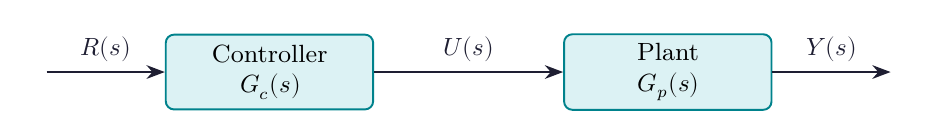
\begin{tikzpicture}[node distance=1.6cm and 2.2cm]
  \node[block] (ctrl) {Controller\\$G_c(s)$};
  \node[block, right=2.4cm of ctrl] (plant) {Plant\\$G_p(s)$};
  \node[left=1.5cm of ctrl]  (in)  {};
  \node[right=1.5cm of plant] (out) {};
  \draw[arrow] (in)    -- node[above]{\small $R(s)$} (ctrl);
  \draw[arrow] (ctrl)  -- node[above]{\small $U(s)$} (plant);
  \draw[arrow] (plant) -- node[above]{\small $Y(s)$} (out);
\end{tikzpicture}
\end{tcolorbox}

$$\frac{Y(s)}{R(s)} = G_c(s)\cdot G_p(s)$$

\subsection{Characteristics of Open Loop Systems}

\begin{tabularx}{\linewidth}{|B{3.2cm}|X|}
\hline
\multicolumn{1}{|>{\centering\arraybackslash}p{3.2cm}|}{\textbf{\color{myred}Feature}} &
\multicolumn{1}{>{\centering\arraybackslash}X|}{\textbf{\color{myred}Open Loop Behaviour}} \\
\hline
Accuracy          & Low — errors from disturbances or parameter changes are not corrected. \\
\hline
Stability         & Generally stable; no feedback loop to introduce phase shift or oscillation. \\
\hline
Complexity        & Simple design; fewer components; easy to maintain. \\
\hline
Cost              & Lower — no sensors, feedback elements, or comparators needed. \\
\hline
Disturbance       & Output permanently affected; no self-correction mechanism. \\
\hline
Calibration       & Must be re-calibrated frequently to maintain accuracy. \\
\hline
Real Examples     & Washing machine (timed cycle), traffic signal timer, electric toaster, stepper motor. \\
\hline
\end{tabularx}

%═══════════════════════════════════════════════════════════════════════════════
\section{Closed Loop (Feedback) Control System}
%═══════════════════════════════════════════════════════════════════════════════

A closed loop system \textbf{continuously monitors the output} and uses the measured value to correct the control action. The difference between reference and actual output is the \textbf{error}, which drives the controller.

\begin{tcolorbox}[defbox]
\textbf{Definition:} A \textbf{closed loop (feedback) control system} is one in which the output is measured, compared with the reference input, and the resulting \textit{error signal} is used to reduce the deviation. Feedback is typically \textbf{negative}.
\end{tcolorbox}

\begin{tcolorbox}[tikzbox, title={Closed Loop Block Diagram (Negative Feedback)}]
\centering
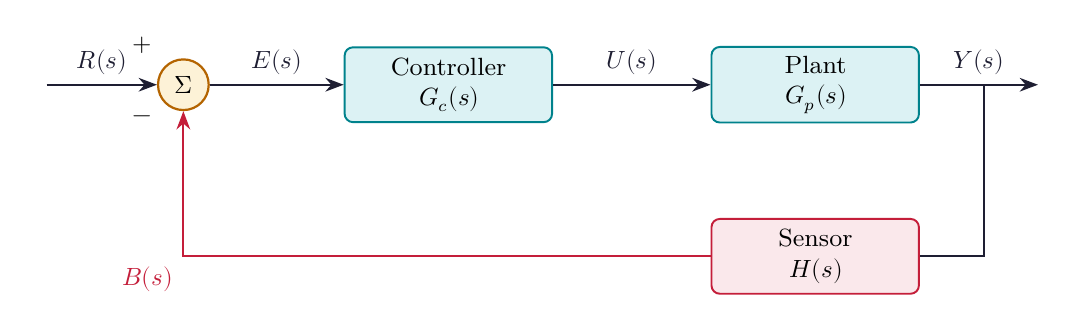
\begin{tikzpicture}[node distance=1.3cm and 1.9cm]
  \node[sumjunc] (sum) {$\Sigma$};
  \node[block, right=1.7cm of sum] (gc)  {Controller\\$G_c(s)$};
  \node[block, right=2.0cm of gc]  (gp)  {Plant\\$G_p(s)$};
  \node[redblock, below=1.2cm of gp](H)  {Sensor\\$H(s)$};
  \node[left=1.4cm of sum]  (ref) {};
  \node[right=1.5cm of gp]  (out) {};
  \draw[arrow]    (ref) -- node[above]{\small $R(s)$}   (sum);
  \draw[arrow]    (sum) -- node[above]{\small $E(s)$}   (gc);
  \draw[arrow]    (gc)  -- node[above]{\small $U(s)$}   (gp);
  \draw[arrow]    (gp)  -- node[above]{\small $Y(s)$}   (out);
  \coordinate (tap) at ($(gp.east)!0.5!(out)$);
  \draw[line]     (tap) |- (H.east);
  \draw[redarrow] (H.west) -| node[below left]{\small $B(s)$} (sum.south);
  \node[above left=1pt and 1pt of sum]{\small $+$};
  \node[below left=1pt and 1pt of sum]{\small $-$};
\end{tikzpicture}
\end{tcolorbox}

\subsection{Closed Loop Transfer Function (CLTF)}

\textbf{Derivation (Unity Feedback, $H(s)=1$):}
\begin{align*}
E(s) &= R(s) - Y(s) \\
Y(s) &= G(s)\cdot E(s) = G(s)\bigl[R(s) - Y(s)\bigr] \\
Y(s)\bigl[1 + G(s)\bigr] &= G(s)\cdot R(s)
\end{align*}

\begin{tcolorbox}[formulabox]
\textbf{Unity Feedback} $\bigl(H(s)=1\bigr)$:
$$\frac{Y(s)}{R(s)} = \frac{G(s)}{1 + G(s)}$$
\textbf{Non-Unity Feedback} $\bigl(H(s)\neq 1\bigr)$:
$$\frac{Y(s)}{R(s)} = \frac{G(s)}{1 + G(s)\,H(s)}, \qquad G(s) = G_c(s)\cdot G_p(s)$$
$G(s)H(s)$ = \textbf{open loop transfer function} (OLTF). \quad $1 + G(s)H(s) = 0$ = \textbf{characteristic equation}.
\end{tcolorbox}

\subsection{Open Loop vs.\ Closed Loop — Comparison}

\begin{tabularx}{\linewidth}{|B{3.0cm}|X|X|}
\hline
\multicolumn{1}{|>{\centering\arraybackslash}p{3.0cm}|}{\textbf{Parameter}} &
\multicolumn{1}{>{\centering\arraybackslash}X|}{\textbf{\color{myamber}Open Loop}} &
\multicolumn{1}{>{\centering\arraybackslash}X|}{\textbf{\color{mygreen}Closed Loop}} \\
\hline
Feedback            & Absent                        & Present (negative) \\
\hline
Accuracy            & Lower                         & Higher \\
\hline
Stability           & More stable                   & May become unstable \\
\hline
Disturbance effect  & High; no correction           & Reduced; self-correcting \\
\hline
Bandwidth           & Narrow                        & Wider \\
\hline
Sensitivity         & High to parameter changes     & Reduced (robust) \\
\hline
Cost \& Complexity  & Low                           & Higher \\
\hline
Real Examples       & Toaster, timer, stepper motor & Thermostat, servo drive, auto-pilot \\
\hline
\end{tabularx}

%═══════════════════════════════════════════════════════════════════════════════
\section{Block Diagram Reduction}
%═══════════════════════════════════════════════════════════════════════════════

A \textbf{block diagram} is a pictorial representation of a control system. For complex multi-loop systems, \textbf{algebraic reduction rules} simplify the diagram step-by-step until a single overall TF $Y(s)/R(s)$ is obtained.

\textbf{Summing junction:} Circle with $+/-$ signs; algebraically adds/subtracts incoming signals.\\
\textbf{Takeoff point:} Node from which the same signal is distributed to multiple branches unchanged.

\begin{tcolorbox}[tikzbox, title={Summing Junction and Takeoff Point}]
\centering
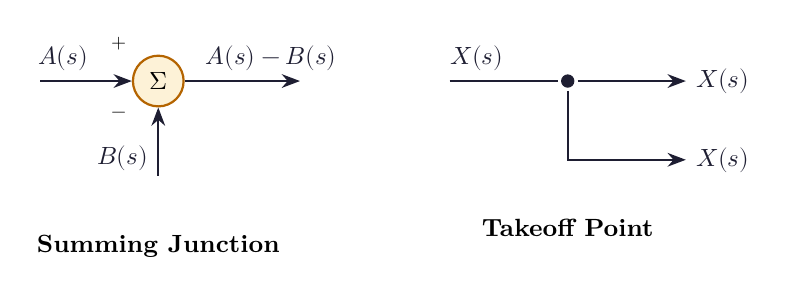
\begin{tikzpicture}[scale=1.0]
  % Summing Junction (Left)
  \begin{scope}[shift={(0,0)}]
    \node[sumjunc] (sum) at (0,0) {$\Sigma$};
    \draw[arrow] (-1.5,0) -- node[above, near start]{\small $A(s)$} (sum);
    \draw[arrow] (0,-1.2) -- node[left, near start]{\small $B(s)$} (sum);
    \draw[arrow] (sum) -- node[above, near end]{\small $A(s) - B(s)$} (1.8,0);
    \node[above left=1pt and 1pt of sum, font=\scriptsize] {$+$};
    \node[below left=1pt and 1pt of sum, font=\scriptsize] {$-$};
    \node[below=1.5cm of sum, font=\small\bfseries] {Summing Junction};
  \end{scope}

  % Takeoff Point (Right)
  \begin{scope}[shift={(5.2,0)}]
    \filldraw[mydark] (0,0) circle (2.2pt) node (pt) {};
    \draw[line] (-1.5,0) -- node[above, near start]{\small $X(s)$} (pt);
    \draw[arrow] (pt) -- (1.5,0) node[right]{\small $X(s)$};
    \draw[arrow] (pt) |- (1.5,-1.0) node[right]{\small $X(s)$};
    \node[below=1.5cm of pt, font=\small\bfseries] {Takeoff Point};
  \end{scope}
\end{tikzpicture}
\end{tcolorbox}

\subsection{Reduction Rules}

\begin{tabularx}{\linewidth}{|B{3.5cm}|X|C{3.0cm}|}
\hline
\multicolumn{1}{|>{\centering\arraybackslash}p{3.5cm}|}{\textbf{\color{myteal}Operation}} &
\multicolumn{1}{>{\centering\arraybackslash}X|}{\textbf{\color{myteal}Description}} &
\multicolumn{1}{>{\centering\arraybackslash}p{3.0cm}|}{\textbf{\color{myteal}Equivalent TF}} \\
\hline
Blocks in Series       & Output of $G_1$ feeds input of $G_2$; same signal chain       & $G_1(s)\cdot G_2(s)$ \\
\hline
Blocks in Parallel     & Same input, individual outputs summed at a junction           & $G_1(s) + G_2(s)$ \\
\hline
Feedback Loop          & Forward path $G$, feedback path $H$ (negative feedback)      & $\dfrac{G}{1+GH}$ \\
\hline
Summing pt.\ forward   & Shift summing junction past block $G$ to the right            & Divide shifted branch by $G$ \\
\hline
Summing pt.\ backward  & Shift summing junction past block $G$ to the left             & Multiply shifted branch by $G$ \\
\hline
Takeoff pt.\ forward   & Shift takeoff past block $G$ to the right                    & Multiply branch by $G$ \\
\hline
Takeoff pt.\ backward  & Shift takeoff past block $G$ to the left                     & Divide branch by $G$ \\
\hline
\end{tabularx}

\subsection{Reduction Procedure (Step-by-Step)}

\begin{enumerate}[label=\textbf{Step \arabic*:}, leftmargin=2.5cm, itemsep=4pt]
  \item Identify and combine all \textbf{cascade (series)} blocks into a single block.
  \item Identify and combine all \textbf{parallel} paths into a single block.
  \item Eliminate all \textbf{feedback loops} using $G/(1 \pm GH)$.
  \item If needed, \textbf{shift} summing junctions or takeoff points to untangle crossed paths.
  \item Repeat steps 1–4 until only a \textbf{single block} $Y(s)/R(s)$ remains.
\end{enumerate}

\begin{tcolorbox}[exambox, title={Exam Tip}]
Always maintain the correct sign ($+/-$) at every summing junction while shifting. Careless sign errors are the most common mistake in block diagram problems.
\end{tcolorbox}

%═══════════════════════════════════════════════════════════════════════════════
\section{Signal Flow Graph (SFG) Analysis}
%═══════════════════════════════════════════════════════════════════════════════

A Signal Flow Graph is an alternative graphical method to represent and solve linear algebraic equations describing a control system. Unlike block diagrams — which require step-by-step reduction — an SFG is solved \textit{directly} using \textbf{Mason's Gain Formula} in a single pass.

\begin{tcolorbox}[masonbox]
\textbf{Definition:} A \textbf{Signal Flow Graph (SFG)} is a directed graph of \textit{nodes} (signals/variables) connected by \textit{directed branches} (carrying gain/transmittance values). It is a compact representation of the system's simultaneous equations.
\end{tcolorbox}

\subsection{Basic Terminology}

\begin{tabularx}{\linewidth}{|B{3.6cm}|X|}
\hline
\multicolumn{1}{|>{\centering\arraybackslash}p{3.6cm}|}{\textbf{\color{mypurple}Term}} &
\multicolumn{1}{>{\centering\arraybackslash}X|}{\textbf{\color{mypurple}Meaning / Definition}} \\
\hline
Node                    & Represents a signal or variable in the system (shown as a small circle). \\
\hline
Branch                  & Directed arrow between two nodes; labelled with the \textit{transmittance} (gain). \\
\hline
Source Node             & Input node — has \textbf{only outgoing} branches; no incoming branches. \\
\hline
Sink Node               & Output node — has \textbf{only incoming} branches; no outgoing branches. \\
\hline
Mixed Node              & A node with both incoming and outgoing branches (intermediate variable). \\
\hline
Forward Path            & Continuous directed path from source to sink in which \textbf{no node is visited more than once}. \\
\hline
Forward Path Gain $P_k$ & Product of all branch gains along the $k$-th forward path. \\
\hline
Loop                    & Closed directed path beginning and ending at the same node, \textbf{no node repeated}. \\
\hline
Loop Gain $L_i$         & Product of all branch gains around the $i$-th loop. \\
\hline
Non-Touching Loops      & Two or more loops that do \textbf{not share any common node}. \\
\hline
\end{tabularx}

\subsection{Mason's Gain Formula}

\begin{tcolorbox}[masonbox]
\centering
$\displaystyle T \;=\; \frac{Y(s)}{R(s)} \;=\; \frac{\displaystyle\sum_{k=1}^{N} P_k\,\Delta_k}{\Delta}$
\end{tcolorbox}

\begin{tabularx}{\linewidth}{|B{2.8cm}|X|}
\hline
\multicolumn{1}{|>{\centering\arraybackslash}p{2.8cm}|}{\textbf{\color{mypurple}Symbol}} &
\multicolumn{1}{>{\centering\arraybackslash}X|}{\textbf{\color{mypurple}Definition}} \\
\hline
$N$              & Total number of forward paths from source to sink. \\
\hline
$P_k$            & Gain of the $k$-th forward path (product of branch gains along that path). \\
\hline
$\Delta$         & Graph determinant $= 1 - \sum_i L_i + \sum_{i,j} L_iL_j - \sum_{i,j,k} L_iL_jL_k + \cdots$ \\
\hline
$\sum L_i$       & Sum of gains of \textbf{all individual loops} in the graph. \\
\hline
$\sum L_iL_j$    & Sum of gain-products of all \textbf{pairs of non-touching loops}. \\
\hline
$\sum L_iL_jL_k$ & Sum of gain-products of all \textbf{triplets of mutually non-touching loops}. \\
\hline
$\Delta_k$       & \textbf{Cofactor} of the $k$-th path: value of $\Delta$ after removing all loops that \textit{touch} forward path $k$. \\
\hline
\end{tabularx}

\subsection{Steps to Apply Mason's Formula}

\begin{enumerate}[label=\textbf{\arabic*.}, leftmargin=*, itemsep=4pt]
  \item \textbf{Identify forward paths:} Trace every path from source to sink (no repeated nodes). Note gain $P_k$ of each.
  \item \textbf{Identify all loops:} Find every closed path. Compute loop gain $L_i$ for each.
  \item \textbf{Find non-touching loop combinations:} Identify all pairs, triplets, etc.\ sharing no common node.
  \item \textbf{Compute graph determinant:} $\Delta = 1 - \sum L_i + \sum L_iL_j - \sum L_iL_jL_k + \cdots$
  \item \textbf{Compute cofactor $\Delta_k$:} For each forward path $k$, remove all loops touching that path from $\Delta$.
  \item \textbf{Apply Mason's formula:} $T = \dfrac{\sum P_k\Delta_k}{\Delta}$.
\end{enumerate}

\subsection{Worked Example — Simple Feedback System}

\begin{tcolorbox}[tikzbox, title={SFG Representation}]
\centering
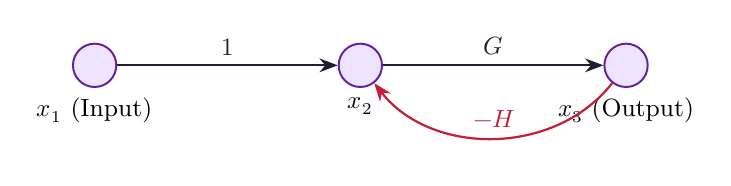
\begin{tikzpicture}[node distance=2.8cm]
  \node[snode, label=below:{\small $x_1$ (Input)}]  (r) {};
  \node[snode, right=of r, label=below:{\small $x_2$}] (e) {};
  \node[snode, right=of e, label=below:{\small $x_3$ (Output)}] (y) {};
  \draw[arrow]             (r) -- node[above]{\small $1$}   (e);
  \draw[arrow]             (e) -- node[above]{\small $G$}   (y);
  \draw[arrow,color=myred] (y) to[bend left=52] node[above]{\small $-H$} (e);
\end{tikzpicture}
\end{tcolorbox}

\textbf{Applying Mason's formula:}
\begin{itemize}[leftmargin=*, itemsep=2pt]
  \item Forward path: $P_1 = 1 \times G = G$
  \item Loop: $L_1 = G \times (-H) = -GH$
  \item No non-touching loop pairs (only one loop).
  \item $\Delta = 1 - L_1 = 1 - (-GH) = 1 + GH$
  \item $\Delta_1 = 1$ \quad (loop $L_1$ touches forward path $P_1$, so removed from $\Delta$)
\end{itemize}

\begin{tcolorbox}[formulabox]
$$T = \frac{P_1\,\Delta_1}{\Delta} = \frac{G \cdot 1}{1 + GH} = \frac{G}{1 + GH} \quad \checkmark$$
Matches the CLTF from block diagram reduction — both methods are equivalent.
\end{tcolorbox}

\subsection{SFG vs.\ Block Diagram — Comparison}

\begin{tabularx}{\linewidth}{|B{3.4cm}|X|X|}
\hline
\multicolumn{1}{|>{\centering\arraybackslash}p{3.4cm}|}{\textbf{Aspect}} &
\multicolumn{1}{>{\centering\arraybackslash}X|}{\textbf{\color{myteal}Block Diagram}} &
\multicolumn{1}{>{\centering\arraybackslash}X|}{\textbf{\color{mypurple}Signal Flow Graph}} \\
\hline
Representation   & Blocks, summing junctions, takeoff points             & Directed nodes and weighted branches \\
\hline
Reduction Method & Step-by-step algebra; multiple passes                 & Mason's formula — single direct computation \\
\hline
Complex Systems  & Tedious; can become cluttered and error-prone          & Compact, systematic, less error-prone \\
\hline
Gain Formula     & No direct formula; reduce iteratively                 & $T = \sum P_k\Delta_k / \Delta$ \\
\hline
Preferred For    & Simple systems; visual understanding                  & Multi-loop systems; quick TF computation \\
\hline
\end{tabularx}

%═══════════════════════════════════════════════════════════════════════════════
% QUICK REVISION PAGE
%═══════════════════════════════════════════════════════════════════════════════
\newpage
\begin{center}
  {\large\bfseries\color{myred} Quick Revision — Module 1}\\[3pt]
  {\small\color{mydark} Control System $|$ EC601}
\end{center}
\noindent{\color{myred}\rule{\linewidth}{1.2pt}}
\vspace{4pt}

\begin{tcolorbox}[formulabox, title={\textbf{Key Formulas at a Glance}}]
\begin{tabularx}{\linewidth}{B{4.5cm} X}
Transfer Function       & $G(s) = Y(s)/U(s)$ \quad (zero initial conditions) \\[2pt]
CLTF (Unity feedback)   & $T(s) = G(s)/[1+G(s)]$ \\[2pt]
CLTF (Non-unity)        & $T(s) = G(s)/[1+G(s)H(s)]$ \\[2pt]
Characteristic Equation & $1 + G(s)H(s) = 0$ \\[2pt]
Series blocks           & $G_{eq} = G_1 \cdot G_2$ \\[2pt]
Parallel blocks         & $G_{eq} = G_1 + G_2$ \\[2pt]
Feedback reduction      & $G_{eq} = G/(1 \pm GH)$ \\[2pt]
Mason's Gain Formula    & $T = \dfrac{\sum_k P_k\Delta_k}{\Delta}$ \\[2pt]
Graph Determinant       & $\Delta = 1 - \sum L_i + \sum L_iL_j - \cdots$
\end{tabularx}
\end{tcolorbox}

\vspace{6pt}

\begin{tcolorbox}[defbox, title={\textbf{One-Line Definitions}}]
\begin{itemize}[leftmargin=*, itemsep=3pt, topsep=0pt]
  \item \textbf{Control System:} Interconnection of components to regulate output to a desired value.
  \item \textbf{Transfer Function:} Ratio of Laplace output to Laplace input at zero initial conditions.
  \item \textbf{Poles:} Roots of denominator of $G(s)$ — determine stability and transient response.
  \item \textbf{Zeros:} Roots of numerator of $G(s)$ — affect frequency response shape.
  \item \textbf{Open Loop:} Control action independent of output; no self-correction.
  \item \textbf{Closed Loop:} Output fed back and compared with reference; error drives controller.
  \item \textbf{Error Signal:} $E(s) = R(s) - B(s)$; difference between reference and feedback.
  \item \textbf{SFG:} Directed graph of nodes and branches representing system equations.
  \item \textbf{Forward Path:} Path from source to sink with no repeated nodes.
  \item \textbf{Loop Gain:} Product of all branch gains around a closed loop.
  \item \textbf{Cofactor $\Delta_k$:} Graph determinant $\Delta$ with all loops touching path $k$ removed.
\end{itemize}
\end{tcolorbox}

\vspace{6pt}

\begin{tcolorbox}[exambox, title={\textbf{Frequently Asked / Viva Points}}]
\begin{enumerate}[leftmargin=*, topsep=0pt, label=\textbf{Q\arabic*.}, itemsep=8pt]
  \item \Q{Why are initial conditions zero in TF?} TF is an input-output model; it characterises the system, not a specific response. Zero I.C.\ ensures the TF is a property of the system alone.
  \item \Q{What is the order of a system?} Highest power of $s$ in the denominator of $G(s)$.
  \item \Q{Difference between open loop and closed loop?} Open loop: no feedback, no self-correction. Closed loop: feedback present, error-driven, self-correcting.
  \item \Q{What is the characteristic equation?} $1 + G(s)H(s) = 0$. Its roots (poles of CLTF) determine stability.
  \item \Q{When is a system proper?} When degree of denominator $\geq$ degree of numerator ($n \geq m$).
  \item \Q{What is a takeoff point?} A node from which the same signal branches to multiple paths without change.
  \item \Q{What is $\Delta_k$ in Mason's formula?} Cofactor of the $k$-th forward path — $\Delta$ computed after removing all loops that touch path $k$.
  \item \Q{Can SFG and block diagram give different results?} No — both are equivalent representations; Mason's formula gives the same TF as block diagram reduction.
  \item \Q{What are non-touching loops?} Loops that share no common node. Their gain products appear in $\Delta$.
  \item \Q{Why is negative feedback preferred?} It reduces error, improves accuracy, reduces sensitivity to parameter variations, and widens bandwidth.
\end{enumerate}
\end{tcolorbox}

\vspace{6pt}

\begin{tcolorbox}[tikzbox, title={\textbf{Comparison Snapshot}}]
\begin{tabularx}{\linewidth}{|B{3.2cm}|X|X|}
\hline
\multicolumn{1}{|>{\centering\arraybackslash}p{3.2cm}|}{\textbf{Property}} &
\multicolumn{1}{>{\centering\arraybackslash}X|}{\textbf{\color{myamber}Open Loop}} &
\multicolumn{1}{>{\centering\arraybackslash}X|}{\textbf{\color{mygreen}Closed Loop}} \\
\hline
Feedback        & No            & Yes (negative) \\
\hline
Accuracy        & Low           & High \\
\hline
Stability       & More stable   & Can oscillate \\
\hline
Cost            & Low           & High \\
\hline
Disturbance     & Not corrected & Self-corrected \\
\hline
\end{tabularx}
\end{tcolorbox}


% -- Module 2 -----------------------------------------------------------------
\modulestart{2}{Stability of Feedback Control Systems}

\section{Stability of Feedback Control Systems}
%═══════════════════════════════════════════════════════════════════════════════

Stability is the most fundamental requirement of any control system. An unstable system produces unbounded output even for a bounded input, making it practically useless.

\begin{tcolorbox}[defbox]
\textbf{BIBO Stability:} A system is \textbf{Bounded-Input Bounded-Output (BIBO) stable} if every bounded input produces a bounded output. For an LTI system, this requires all poles of the closed-loop transfer function to lie in the \textbf{left half of the $s$-plane} (i.e., have negative real parts).
\end{tcolorbox}

\subsection{Stability Conditions}

\begin{tabularx}{\linewidth}{|B{3.2cm}|X|}
\hline
\multicolumn{1}{|>{\centering\arraybackslash}p{3.2cm}|}{\textbf{\color{myteal}Condition}} &
\multicolumn{1}{>{\centering\arraybackslash}X|}{\textbf{\color{myteal}Meaning}} \\
\hline
Stable & All closed-loop poles have \textbf{negative real parts} (left half $s$-plane). Output decays to zero. \\
\hline
Marginally Stable & Poles on the \textbf{imaginary axis} (zero real part). Output oscillates with constant amplitude. \\
\hline
Unstable & At least one pole in the \textbf{right half $s$-plane}. Output grows without bound. \\
\hline
\end{tabularx}

\subsection{Relative Stability}

Absolute stability only tells us \textit{whether} a system is stable. \textbf{Relative stability} tells us \textit{how stable} — i.e., how far the closed-loop poles are from the imaginary axis.

\begin{tcolorbox}[defbox]
\textbf{Relative Stability:} A measure of the degree of stability. A system with poles far into the left half-plane is \textit{more stable} (faster decay, less oscillation) than one with poles close to the imaginary axis. Quantified by \textbf{gain margin} and \textbf{phase margin} (covered in Module 3).
\end{tcolorbox}

\begin{tcolorbox}[formulabox, title={Key Concept}]
If all poles of $T(s) = \dfrac{G(s)}{1+G(s)H(s)}$ satisfy $\text{Re}(s_i) < 0$, the system is stable.\\[4pt]
The \textbf{characteristic equation} $1 + G(s)H(s) = 0$ determines the pole locations.
\end{tcolorbox}

%═══════════════════════════════════════════════════════════════════════════════
\section{Routh–Hurwitz Stability Criterion}
%═══════════════════════════════════════════════════════════════════════════════

The Routh–Hurwitz criterion determines stability \textbf{without solving} the characteristic equation. It counts the number of roots in the right half $s$-plane using a tabular method.

\begin{tcolorbox}[defbox]
\textbf{Definition:} The \textbf{Routh–Hurwitz criterion} states that a system is stable if and only if all elements of the \textbf{first column} of the Routh array are \textbf{positive}. The number of sign changes in the first column equals the number of closed-loop poles in the right half $s$-plane.
\end{tcolorbox}

\subsection{Constructing the Routh Array}

Given the characteristic equation:
$$a_n s^n + a_{n-1}s^{n-1} + \cdots + a_1 s + a_0 = 0$$

\textbf{Step 1 — Necessary condition:} All coefficients $a_i$ must be present and have the \textbf{same sign}. If any coefficient is zero or negative, the system is \textit{unstable or marginally stable} (no need to proceed).

\textbf{Step 2 — Form the array:}

\begin{tcolorbox}[tikzbox, title={Routh Array Structure}]
\centering
\renewcommand{\arraystretch}{1.4}
\begin{tabular}{c|cccc}
$s^n$     & $a_n$     & $a_{n-2}$ & $a_{n-4}$ & $\cdots$ \\
$s^{n-1}$ & $a_{n-1}$ & $a_{n-3}$ & $a_{n-5}$ & $\cdots$ \\
$s^{n-2}$ & $b_1$     & $b_2$     & $b_3$     & $\cdots$ \\
$s^{n-3}$ & $c_1$     & $c_2$     & $c_3$     & $\cdots$ \\
$\vdots$  & $\vdots$  & $\vdots$  &           &          \\
$s^0$     & $a_0$     &           &           &          \\
\end{tabular}
\end{tcolorbox}

\begin{tcolorbox}[formulabox, title={Row Computation Formulas}]
$$b_1 = \frac{a_{n-1}\cdot a_{n-2} - a_n\cdot a_{n-3}}{a_{n-1}}, \quad
  b_2 = \frac{a_{n-1}\cdot a_{n-4} - a_n\cdot a_{n-5}}{a_{n-1}}, \quad \ldots$$
$$c_1 = \frac{b_1\cdot a_{n-3} - a_{n-1}\cdot b_2}{b_1}, \quad
  c_2 = \frac{b_1\cdot a_{n-5} - a_{n-1}\cdot b_3}{b_1}, \quad \ldots$$
Continue until all rows are complete. \textbf{Stability:} No sign changes in column 1.
\end{tcolorbox}

\subsection{Special Cases}

\begin{tabularx}{\linewidth}{|B{3.4cm}|X|}
\hline
\multicolumn{1}{|>{\centering\arraybackslash}p{3.4cm}|}{\textbf{\color{myred}Special Case}} &
\multicolumn{1}{>{\centering\arraybackslash}X|}{\textbf{\color{myred}Handling}} \\
\hline
Zero in first column & Replace zero with small $\varepsilon > 0$, complete the array, then let $\varepsilon \to 0^+$. Count sign changes. \\
\hline
Entire row of zeros & System has symmetric roots (pairs on imaginary axis or real axis). Form \textbf{auxiliary polynomial} from the row above, differentiate it, and use its coefficients to replace the zero row. \\
\hline
\end{tabularx}

\subsection{Worked Example}

\begin{tcolorbox}[examplebox, title={Example — 3rd Order System}]
\textbf{Characteristic equation:} $s^3 + 2s^2 + 4s + 8 = 0$

\textbf{Routh Array:}
\renewcommand{\arraystretch}{1.3}
\begin{center}
\begin{tabular}{c|cc}
$s^3$ & $1$ & $4$ \\
$s^2$ & $2$ & $8$ \\
$s^1$ & $b_1 = \dfrac{2\times4 - 1\times8}{2} = \dfrac{0}{2} = 0$ & $0$ \\
$s^0$ & $8$ & \\
\end{tabular}
\end{center}

$b_1 = 0$ → zero in first column → replace with $\varepsilon$, let $\varepsilon\to 0^+$.\\
First column: $1,\ 2,\ \varepsilon,\ 8$ — as $\varepsilon\to 0^+$, no sign change.\\
\textbf{Result:} Marginally stable (one pair of roots on imaginary axis at $s = \pm j2$).
\end{tcolorbox}

\begin{tcolorbox}[exambox, title={Exam Tips — Routh Criterion}]
\begin{itemize}[leftmargin=*, itemsep=3pt, topsep=0pt]
  \item \textbf{Necessary condition first:} All coefficients positive and non-zero — check before building the array.
  \item \textbf{Number of sign changes} in column 1 = number of unstable poles.
  \item \textbf{Marginal stability:} Entire row of zeros → auxiliary polynomial roots on $j\omega$-axis.
  \item \textbf{Range of $K$ for stability:} Set up array with $K$, find condition on first column $> 0$.
  \item Routh criterion gives \textit{no information} about the actual pole locations — only their count in RHP.
\end{itemize}
\end{tcolorbox}

%═══════════════════════════════════════════════════════════════════════════════
\section{Steady-State Error (SSE)}
%═══════════════════════════════════════════════════════════════════════════════

Even a stable system may not track the reference input perfectly in steady state. The \textbf{steady-state error} quantifies this residual deviation after all transients have died out.

\begin{tcolorbox}[defbox]
\textbf{Definition:} The \textbf{steady-state error} $e_{ss}$ is the difference between the desired reference input and the actual output as $t \to \infty$:
$$e_{ss} = \lim_{t\to\infty} e(t) = \lim_{s\to 0}\, s\,E(s)$$
where $E(s) = \dfrac{R(s)}{1 + G(s)H(s)}$ for a unity-feedback system.
\end{tcolorbox}

\subsection{System Type Number}

The \textbf{type number} of a system is the number of open-loop poles at the origin (i.e., the number of pure integrators in $G(s)H(s)$).

$$G(s)H(s) = \frac{K\,(1+T_1 s)(1+T_2 s)\cdots}{s^N\,(1+T_a s)(1+T_b s)\cdots}$$

Here $N$ is the \textbf{type number} (0, 1, 2, \ldots). More integrators → better steady-state tracking.

\subsection{Error Constants and SSE Formulas}

\begin{tabularx}{\linewidth}{|B{2.8cm}|>{\centering\arraybackslash}X|>{\centering\arraybackslash}X|>{\centering\arraybackslash}X|}
\hline
\multicolumn{1}{|>{\centering\arraybackslash}p{2.8cm}|}{\textbf{\color{myteal}Input}} &
\textbf{\color{myteal}Type 0} & \textbf{\color{myteal}Type 1} & \textbf{\color{myteal}Type 2} \\
\hline
Step $R(s)=\frac{1}{s}$       & $\dfrac{1}{1+K_p}$ & $0$              & $0$ \\
\hline
Ramp $R(s)=\frac{1}{s^2}$     & $\infty$           & $\dfrac{1}{K_v}$ & $0$ \\
\hline
Parabola $R(s)=\frac{1}{s^3}$ & $\infty$           & $\infty$         & $\dfrac{1}{K_a}$ \\
\hline
\end{tabularx}

\begin{tcolorbox}[formulabox, title={Error Constants}]
$$K_p = \lim_{s\to 0} G(s)H(s) \quad \text{(Position constant)}$$
$$K_v = \lim_{s\to 0}\, s\,G(s)H(s) \quad \text{(Velocity constant)}$$
$$K_a = \lim_{s\to 0}\, s^2\,G(s)H(s) \quad \text{(Acceleration constant)}$$
\end{tcolorbox}

\subsection{Steady-State Accuracy}

\begin{tcolorbox}[defbox]
\textbf{Steady-State Accuracy} is the ability of a control system to track the reference input with minimum error in steady state. It is directly related to the \textbf{type number} and the \textbf{gain} of the open-loop transfer function. Higher type number and higher gain both improve steady-state accuracy.
\end{tcolorbox}

\begin{tcolorbox}[exambox, title={Exam Tips — SSE}]
\begin{itemize}[leftmargin=*, itemsep=3pt, topsep=0pt]
  \item SSE depends on \textbf{system type} and \textbf{input type} — memorise the table above.
  \item Increasing open-loop gain $K$ reduces SSE for the same type, but may reduce stability.
  \item Adding an integrator (increasing type) eliminates SSE for lower-order inputs but risks instability.
  \item For \textbf{non-unity feedback}, use $E(s) = R(s) - C(s)$ and apply final value theorem carefully.
  \item \textbf{Final Value Theorem} valid only if $sE(s)$ has all poles in LHP (system must be stable).
\end{itemize}
\end{tcolorbox}

%═══════════════════════════════════════════════════════════════════════════════
\section{Disturbance Rejection, Sensitivity and Robustness}
%═══════════════════════════════════════════════════════════════════════════════

\subsection{Disturbance Rejection}

Real systems are subject to unwanted inputs (disturbances) such as load changes, noise, and environmental variations. A good control system must \textbf{reject disturbances} — i.e., minimise their effect on the output.

\begin{tcolorbox}[defbox]
\textbf{Disturbance Rejection:} The ability of a closed-loop system to suppress the effect of disturbance inputs $D(s)$ on the output $Y(s)$. The \textbf{disturbance transfer function} is:
$$\frac{Y(s)}{D(s)}\bigg|_{R=0} = \frac{G_p(s)}{1 + G_c(s)G_p(s)H(s)}$$
High controller gain $G_c(s)$ reduces this ratio, improving disturbance rejection.
\end{tcolorbox}

\begin{tcolorbox}[tikzbox, title={Closed Loop with Disturbance}]
\centering
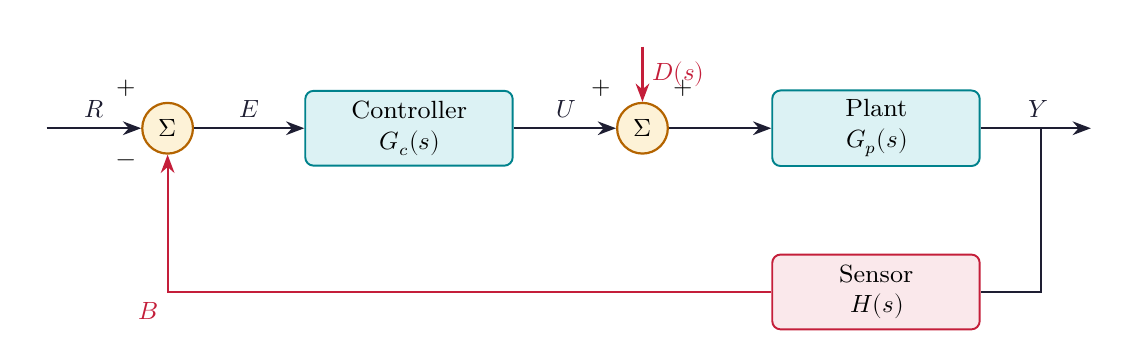
\begin{tikzpicture}[node distance=0.5cm and 1.6cm]
  \node[sumjunc] (sum1) {$\Sigma$};
  \node[block, right=1.4cm of sum1] (gc) {Controller\\$G_c(s)$};
  \node[sumjunc, right=1.3cm of gc] (sum2) {$\Sigma$};
  \node[block, right=1.3cm of sum2] (gp) {Plant\\$G_p(s)$};
  \node[redblock, below=1.1cm of gp] (H) {Sensor\\$H(s)$};
  \node[left=1.2cm of sum1] (ref) {};
  \node[right=1.4cm of gp]  (out) {};
  \node[above=0.7cm of sum2] (dist) {};

  \draw[arrow] (ref)  -- node[above]{\small $R$}   (sum1);
  \draw[arrow] (sum1) -- node[above]{\small $E$}   (gc);
  \draw[arrow] (gc)   -- node[above]{\small $U$}   (sum2);
  \draw[arrow] (sum2) -- (gp);
  \draw[arrow] (gp)   -- node[above]{\small $Y$}   (out);
  \draw[redarrow] (dist) -- node[right]{\small $D(s)$} (sum2);
  \coordinate (tap) at ($(gp.east)!0.5!(out)$);
  \draw[line]  (tap) |- (H.east);
  \draw[redarrow] (H.west) -| node[below left]{\small $B$} (sum1.south);
  \node[above left=1pt and 1pt of sum1]{\small $+$};
  \node[below left=1pt and 1pt of sum1]{\small $-$};
  \node[above left=1pt and 1pt of sum2]{\small $+$};
  \node[above right=1pt and 1pt of sum2]{\small $+$};
\end{tikzpicture}
\end{tcolorbox}

\subsection{Sensitivity}

\begin{tcolorbox}[defbox]
\textbf{Sensitivity Function} $S(s)$: Measures how much the closed-loop transfer function $T(s)$ changes relative to changes in the plant $G(s)$:
$$S(s) = \frac{1}{1 + G(s)H(s)}$$
\textbf{Complementary Sensitivity} $T(s) = 1 - S(s) = \dfrac{G(s)H(s)}{1+G(s)H(s)}$\\[4pt]
Note: $S(s) + T(s) = 1$ always. High loop gain $\Rightarrow$ $S \approx 0$ (low sensitivity).
\end{tcolorbox}

\subsection{Robustness}

\begin{tcolorbox}[defbox]
\textbf{Robustness:} The ability of a control system to maintain acceptable performance despite \textit{uncertainties} in the plant model (parameter variations, unmodelled dynamics, external disturbances). A robust system has:
\begin{itemize}[leftmargin=*, itemsep=2pt, topsep=2pt]
  \item Low sensitivity to plant parameter changes
  \item Good disturbance rejection
  \item Adequate gain and phase margins
\end{itemize}
\end{tcolorbox}

\begin{tabularx}{\linewidth}{|B{3.2cm}|X|X|}
\hline
\multicolumn{1}{|>{\centering\arraybackslash}p{3.2cm}|}{\textbf{Property}} &
\multicolumn{1}{>{\centering\arraybackslash}X|}{\textbf{\color{myamber}Open Loop}} &
\multicolumn{1}{>{\centering\arraybackslash}X|}{\textbf{\color{mygreen}Closed Loop}} \\
\hline
Sensitivity to $\Delta G$ & High — directly affects output & Reduced by factor $1+GH$ \\
\hline
Disturbance rejection & None & Good (high gain helps) \\
\hline
Robustness & Poor & Better (with proper design) \\
\hline
Bandwidth & Narrow & Wider \\
\hline
\end{tabularx}

%═══════════════════════════════════════════════════════════════════════════════
\section{PID Controllers}
%═══════════════════════════════════════════════════════════════════════════════

A \textbf{PID controller} combines three control actions — Proportional, Integral, and Derivative — to achieve fast response, zero steady-state error, and good damping simultaneously.

\begin{tcolorbox}[formulabox, title={PID Control Law (Time Domain)}]
$$u(t) = K_p\,e(t) \;+\; K_i\int_0^t e(\tau)\,d\tau \;+\; K_d\,\frac{de(t)}{dt}$$
\textbf{Transfer Function (s-domain):}
$$G_c(s) = K_p + \frac{K_i}{s} + K_d s = \frac{K_d s^2 + K_p s + K_i}{s}$$
\end{tcolorbox}

\subsection{Proportional (P) Controller}

\begin{tcolorbox}[defbox]
\textbf{P Controller:} $u(t) = K_p\,e(t)$, \quad $G_c(s) = K_p$\\[3pt]
Output is proportional to the current error. Increasing $K_p$ reduces SSE but increases overshoot and may cause instability.
\end{tcolorbox}

\begin{tabularx}{\linewidth}{|B{3.4cm}|X|}
\hline
\multicolumn{1}{|>{\centering\arraybackslash}p{3.4cm}|}{\textbf{\color{mygreen}Effect of increasing $K_p$}} &
\multicolumn{1}{>{\centering\arraybackslash}X|}{\textbf{\color{mygreen}Result}} \\
\hline
Rise time         & Decreases \\
\hline
Overshoot         & Increases \\
\hline
Settling time     & Small change \\
\hline
Steady-state error & Decreases (but never zero for Type 0) \\
\hline
Stability         & Degrades at very high $K_p$ \\
\hline
\end{tabularx}

\subsection{Integral (I) Controller}

\begin{tcolorbox}[defbox]
\textbf{I Controller:} $u(t) = K_i\int e(t)\,dt$, \quad $G_c(s) = K_i/s$\\[3pt]
Integrates the error over time. Eliminates steady-state error completely (adds a pole at origin, increasing system type by 1). However, it slows the response and can cause instability (integral windup).
\end{tcolorbox}

\subsection{Derivative (D) Controller}

\begin{tcolorbox}[defbox]
\textbf{D Controller:} $u(t) = K_d\,\dfrac{de}{dt}$, \quad $G_c(s) = K_d s$\\[3pt]
Responds to the \textit{rate of change} of error — anticipates future error. Improves damping and reduces overshoot. \textbf{Never used alone} (amplifies noise; no steady-state correction). Always combined with P or PI.
\end{tcolorbox}

\subsection{Combined PID — Effect Summary}

\begin{tabularx}{\linewidth}{|>{\bfseries\raggedright\arraybackslash}p{1.8cm}|>{\centering\arraybackslash}X|>{\centering\arraybackslash}X|>{\centering\arraybackslash}X|>{\centering\arraybackslash}X|}
\hline
\multicolumn{1}{|>{\centering\arraybackslash}p{1.8cm}|}{\textbf{Controller}} &
\textbf{Rise Time} & \textbf{Overshoot} & \textbf{Settling} & \textbf{SSE} \\
\hline
P   & Decrease       & Increase  & Small $\Delta$ & Decrease  \\
\hline
I   & Decrease       & Increase  & Increase       & Eliminate \\
\hline
D   & Small $\Delta$ & Decrease  & Decrease       & No effect \\
\hline
PI  & Decrease       & Increase  & Increase       & Eliminate \\
\hline
PD  & Decrease       & Decrease  & Decrease       & No effect \\
\hline
PID & Decrease       & Decrease  & Decrease       & Eliminate \\
\hline
\end{tabularx}

\begin{tcolorbox}[exambox, title={Exam Tips — PID}]
\begin{itemize}[leftmargin=*, itemsep=3pt, topsep=0pt]
  \item \textbf{P alone:} Always has residual SSE for Type 0 systems.
  \item \textbf{I action:} Eliminates SSE but causes \textit{integral windup} — output saturates if error persists.
  \item \textbf{D action:} Improves transient response; \textbf{never used alone} — amplifies high-frequency noise.
  \item \textbf{PID transfer function} has a zero at origin (from $K_i/s$) and two zeros from numerator.
  \item \textbf{Ziegler–Nichols method} is the standard tuning technique for PID (may appear in viva).
\end{itemize}
\end{tcolorbox}

%═══════════════════════════════════════════════════════════════════════════════
\section{Realization of PID Controllers}
%═══════════════════════════════════════════════════════════════════════════════

\subsection{Op-Amp Realization}

Op-amp circuits implement P, I, D, and PID actions using resistors and capacitors. The inverting op-amp configuration is standard.

\subsubsection*{Proportional Controller}

\begin{tcolorbox}[tikzbox, title={P Controller — Inverting Amplifier}]
\centering
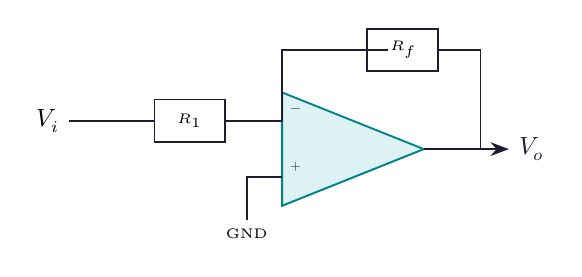
\begin{tikzpicture}[scale=0.9]
  % Op-amp symbol
  \draw[line width=0.7pt, draw=myteal, fill=hdrteal]
    (3,0) -- (3,1.6) -- (5,0.8) -- cycle;
  % Input resistor R1
  \draw[line width=0.7pt, color=mydark] (0,1.2) -- (1.2,1.2);
  \draw[line width=0.7pt, color=mydark] (1.2,0.9) rectangle (2.2,1.5);
  \node at (1.7,1.2) [font=\tiny] {$R_1$};
  \draw[line width=0.7pt, color=mydark] (2.2,1.2) -- (3,1.2);
  % Feedback resistor Rf
  \draw[line width=0.7pt, color=mydark] (3,1.2) -- (3,2.2) -- (4.5,2.2);
  \draw[line width=0.7pt, color=mydark] (4.2,1.9) rectangle (5.2,2.5);
  \node at (4.7,2.2) [font=\tiny] {$R_f$};
  \draw[line width=0.7pt, color=mydark] (5.2,2.2) -- (5.8,2.2) -- (5.8,0.8);
  % Non-inverting to ground
  \draw[line width=0.7pt, color=mydark] (3,0.4) -- (2.5,0.4) -- (2.5,-0.2);
  \node at (2.5,-0.4) [font=\tiny] {GND};
  % Output
  \draw[arrow] (5,0.8) -- (6.2,0.8) node[right,font=\small] {$V_o$};
  % Input label
  \node at (-0.3,1.2) [font=\small] {$V_i$};
  % Labels
  \node at (3.2,1.35) [font=\tiny,color=mydark] {$-$};
  \node at (3.2,0.55) [font=\tiny,color=mydark] {$+$};
\end{tikzpicture}
$$G_c(s) = -\frac{R_f}{R_1} = -K_p \qquad (K_p = R_f/R_1)$$
\end{tcolorbox}

\subsubsection*{PI Controller}

Replace $R_f$ with a series combination of $R_f$ and capacitor $C_f$:

\begin{tcolorbox}[formulabox, title={PI Controller — Op-Amp Transfer Function}]
$$G_c(s) = -\frac{Z_f}{Z_1} = -\frac{R_f + 1/(sC_f)}{R_1} = -\left(\frac{R_f}{R_1} + \frac{1}{sR_1C_f}\right) = -\left(K_p + \frac{K_i}{s}\right)$$
$$K_p = \frac{R_f}{R_1}, \qquad K_i = \frac{1}{R_1 C_f}$$
\end{tcolorbox}

\subsubsection*{PD Controller}

Replace input $R_1$ with a series combination of $R_1$ and capacitor $C_1$:

\begin{tcolorbox}[formulabox, title={PD Controller — Op-Amp Transfer Function}]
$$G_c(s) = -\frac{R_f}{R_1 + 1/(sC_1)} = -\frac{sR_fC_1}{1 + sR_1C_1} \approx -(K_p + K_d s) \text{ for small }R_1$$
$$K_p = \frac{R_f}{R_1}, \qquad K_d = R_f C_1$$
\end{tcolorbox}

\subsubsection*{PID Controller (Op-Amp)}

\begin{tcolorbox}[formulabox, title={PID Controller — Op-Amp Transfer Function}]
Use $Z_1 = R_1 + 1/(sC_1)$ as input impedance and $Z_f = R_f \| (1/sC_f)$ as feedback impedance:
$$G_c(s) = -\frac{Z_f}{Z_1} = -\frac{R_f/(1+sR_fC_f)}{R_1 + 1/(sC_1)}$$
Simplified ideal form:
$$G_c(s) = -\left(K_p + \frac{K_i}{s} + K_d s\right)$$
$$K_p = \frac{R_f}{R_1},\quad K_i = \frac{1}{R_1 C_f},\quad K_d = R_f C_1$$
The negative sign is corrected by cascading an inverting unity-gain stage.
\end{tcolorbox}

\subsection{Digital Implementation of PID}

In digital (discrete-time) systems, the PID algorithm is implemented in software using numerical approximations of integration and differentiation.

\begin{tcolorbox}[defbox]
\textbf{Discrete PID Algorithm:} With sampling period $T_s$, the continuous PID is discretised as:
\begin{itemize}[leftmargin=*, itemsep=2pt, topsep=2pt]
  \item \textbf{Proportional:} $P[k] = K_p\,e[k]$
  \item \textbf{Integral} (rectangular/trapezoidal): $I[k] = I[k-1] + K_i\,T_s\,e[k]$
  \item \textbf{Derivative} (backward difference): $D[k] = K_d\,\dfrac{e[k]-e[k-1]}{T_s}$
  \item \textbf{Output:} $u[k] = P[k] + I[k] + D[k]$
\end{itemize}
\end{tcolorbox}

\begin{tcolorbox}[formulabox, title={Pulse Transfer Function (Z-domain)}]
Using backward Euler ($s \approx \dfrac{z-1}{T_s z}$):
$$G_c(z) = K_p + K_i\frac{T_s z}{z-1} + K_d\frac{z-1}{T_s z}$$
\end{tcolorbox}

\begin{tabularx}{\linewidth}{|B{3.2cm}|X|X|}
\hline
\multicolumn{1}{|>{\centering\arraybackslash}p{3.2cm}|}{\textbf{Aspect}} &
\multicolumn{1}{>{\centering\arraybackslash}X|}{\textbf{\color{myamber}Analog (Op-Amp)}} &
\multicolumn{1}{>{\centering\arraybackslash}X|}{\textbf{\color{mygreen}Digital (Microcontroller)}} \\
\hline
Implementation  & Hardware (R, C, op-amp)       & Software (algorithm in MCU/DSP) \\
\hline
Tuning          & Change component values       & Change $K_p$, $K_i$, $K_d$ in code \\
\hline
Noise           & Susceptible to component drift & Quantisation noise; sampling delay \\
\hline
Flexibility     & Fixed once built              & Easily reprogrammable \\
\hline
Cost            & Low for simple systems        & Higher (processor needed) \\
\hline
\end{tabularx}

%═══════════════════════════════════════════════════════════════════════════════
\section{Feed-Forward Control}
%═══════════════════════════════════════════════════════════════════════════════

\begin{tcolorbox}[defbox]
\textbf{Feed-Forward Control:} A control strategy in which the controller acts on a \textit{measured disturbance} or the \textit{reference input directly}, before the disturbance affects the output. It does \textbf{not} use feedback — it anticipates and cancels the disturbance proactively.
\end{tcolorbox}

\begin{tcolorbox}[tikzbox, title={Feed-Forward + Feedback Configuration}]
\centering
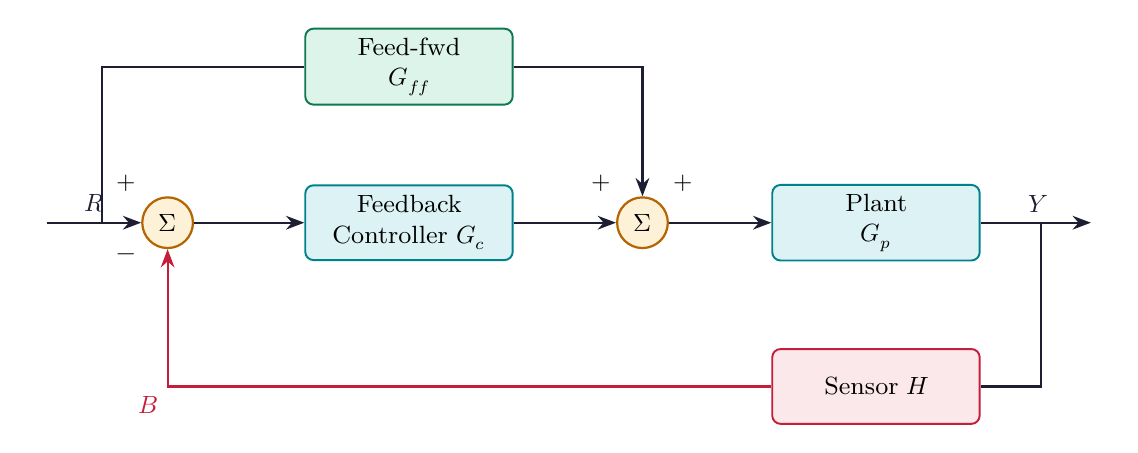
\begin{tikzpicture}[node distance=0.5cm and 1.5cm]
  \node[sumjunc] (sum1) {$\Sigma$};
  \node[block, right=1.4cm of sum1] (gc) {Feedback\\Controller $G_c$};
  \node[sumjunc, right=1.3cm of gc] (sum2) {$\Sigma$};
  \node[block, right=1.3cm of sum2] (gp) {Plant\\$G_p$};
  \node[greenblock, above=1.0cm of gc] (gff) {Feed-fwd\\$G_{ff}$};
  \node[redblock, below=1.1cm of gp] (H) {Sensor $H$};
  \node[left=1.2cm of sum1] (ref) {};
  \node[right=1.4cm of gp]  (out) {};

  \draw[arrow] (ref)  -- node[above]{\small $R$} (sum1);
  \draw[arrow] (sum1) -- (gc);
  \draw[arrow] (gc)   -- (sum2);
  \draw[arrow] (sum2) -- (gp);
  \draw[arrow] (gp)   -- node[above]{\small $Y$} (out);
  % Feed-forward path
  \coordinate (reftap) at ($(ref)!0.5!(sum1)$);
  \draw[line]  (reftap) |- (gff.west);
  \draw[arrow] (gff.east) -| (sum2.north);
  % Feedback
  \coordinate (tap) at ($(gp.east)!0.5!(out)$);
  \draw[line]  (tap) |- (H.east);
  \draw[redarrow] (H.west) -| node[below left]{\small $B$} (sum1.south);
  \node[above left=1pt and 1pt of sum1]{\small $+$};
  \node[below left=1pt and 1pt of sum1]{\small $-$};
  \node[above left=1pt and 1pt of sum2]{\small $+$};
  \node[above right=1pt and 1pt of sum2]{\small $+$};
\end{tikzpicture}
\end{tcolorbox}

\begin{tcolorbox}[formulabox, title={Ideal Feed-Forward Condition}]
For perfect disturbance cancellation, the feed-forward controller should satisfy:
$$G_{ff}(s) = -\frac{G_d(s)}{G_p(s)}$$
where $G_d(s)$ is the disturbance transfer function and $G_p(s)$ is the plant. In practice, exact cancellation is impossible due to model uncertainty — hence feedback is always retained alongside feed-forward.
\end{tcolorbox}

\begin{tabularx}{\linewidth}{|B{3.2cm}|X|X|}
\hline
\multicolumn{1}{|>{\centering\arraybackslash}p{3.2cm}|}{\textbf{Aspect}} &
\multicolumn{1}{>{\centering\arraybackslash}X|}{\textbf{\color{myamber}Feedback Only}} &
\multicolumn{1}{>{\centering\arraybackslash}X|}{\textbf{\color{mygreen}Feed-Forward + Feedback}} \\
\hline
Disturbance handling & Reacts after output is affected & Anticipates and cancels disturbance \\
\hline
Model dependency & Low (error-driven) & High (needs accurate plant model) \\
\hline
Stability risk & Inherent (loop gain) & Lower (FF is open-loop) \\
\hline
Typical use & General purpose & Known, measurable disturbances \\
\hline
\end{tabularx}

%═══════════════════════════════════════════════════════════════════════════════
\section{Multi-Loop Control Configurations}
%═══════════════════════════════════════════════════════════════════════════════

\begin{tcolorbox}[defbox]
\textbf{Multi-Loop Control:} Control architectures that use more than one feedback loop to improve performance. The most common configurations are \textbf{cascade (series)} control and \textbf{ratio control}.
\end{tcolorbox}

\subsection{Cascade (Inner–Outer Loop) Control}

\begin{tcolorbox}[defbox]
\textbf{Cascade Control:} Two feedback loops — an \textbf{inner (secondary) loop} and an \textbf{outer (primary) loop}. The output of the outer controller becomes the \textit{set-point} for the inner controller. The inner loop handles fast disturbances; the outer loop handles the primary variable.
\end{tcolorbox}

\begin{tcolorbox}[tikzbox, title={Cascade Control Block Diagram}]
\centering
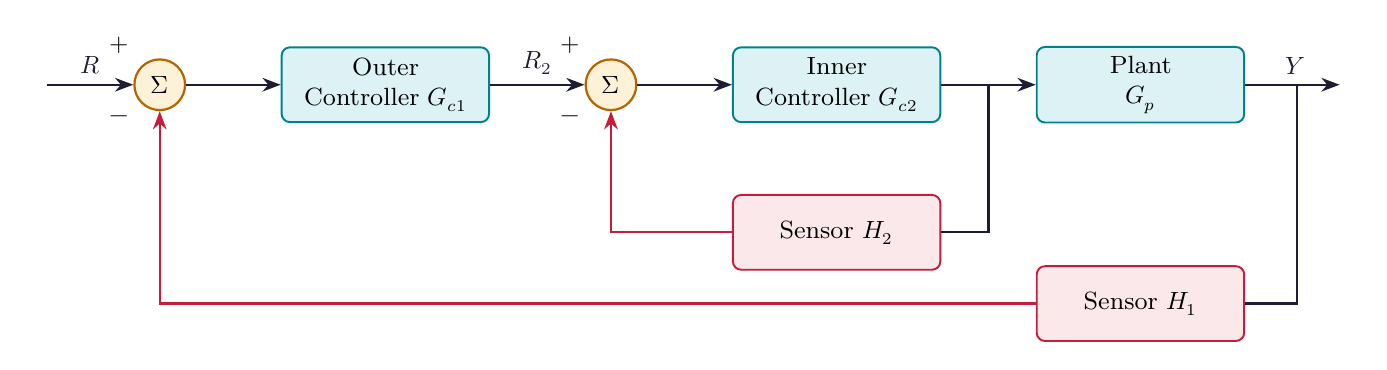
\begin{tikzpicture}[node distance=0.5cm and 1.3cm]
  \node[sumjunc] (sum1) {$\Sigma$};
  \node[block, right=1.2cm of sum1] (gc1) {Outer\\Controller $G_{c1}$};
  \node[sumjunc, right=1.2cm of gc1] (sum2) {$\Sigma$};
  \node[block, right=1.2cm of sum2] (gc2) {Inner\\Controller $G_{c2}$};
  \node[block, right=1.2cm of gc2]  (gp)  {Plant\\$G_p$};
  \node[redblock, below=0.9cm of gc2] (H2) {Sensor $H_2$};
  \node[redblock, below=1.8cm of gp]  (H1) {Sensor $H_1$};
  \node[left=1.1cm of sum1] (ref) {};
  \node[right=1.2cm of gp]  (out) {};

  \draw[arrow] (ref)  -- node[above]{\small $R$}  (sum1);
  \draw[arrow] (sum1) -- (gc1);
  \draw[arrow] (gc1)  -- node[above]{\small $R_2$} (sum2);
  \draw[arrow] (sum2) -- (gc2);
  \draw[arrow] (gc2)  -- (gp);
  \draw[arrow] (gp)   -- node[above]{\small $Y$}  (out);
  % Inner feedback
  \coordinate (tap2) at ($(gc2.east)!0.5!(gp.west)$);
  \draw[line]  (tap2) |- (H2.east);
  \draw[redarrow] (H2.west) -| (sum2.south);
  % Outer feedback
  \coordinate (tap1) at ($(gp.east)!0.5!(out)$);
  \draw[line]  (tap1) |- (H1.east);
  \draw[redarrow] (H1.west) -| (sum1.south);
  \node[above left=1pt and 1pt of sum1]{\small $+$};
  \node[below left=1pt and 1pt of sum1]{\small $-$};
  \node[above left=1pt and 1pt of sum2]{\small $+$};
  \node[below left=1pt and 1pt of sum2]{\small $-$};
\end{tikzpicture}
\end{tcolorbox}

\textbf{Advantages of Cascade Control:}
\begin{itemize}[leftmargin=*, itemsep=2pt]
  \item Inner loop rejects disturbances \textit{before} they propagate to the outer loop.
  \item Faster overall response — inner loop is tuned for speed.
  \item Outer loop can be tuned independently for accuracy.
\end{itemize}

\subsection{Ratio Control}

\begin{tcolorbox}[defbox]
\textbf{Ratio Control:} Maintains a fixed ratio between two process variables (e.g., fuel-to-air ratio in a combustion system). One variable is the \textit{wild} (uncontrolled) stream; the other is the \textit{controlled} stream adjusted to maintain the ratio.
$$\text{Set-point of controlled stream} = K_r \times \text{(measured wild stream)}$$
\end{tcolorbox}

%═══════════════════════════════════════════════════════════════════════════════
% QUICK REVISION — MODULE 2
%═══════════════════════════════════════════════════════════════════════════════
\newpage
\begin{center}
  {\large\bfseries\color{myred} Quick Revision — Module 2}\\[3pt]
  {\small\color{mydark} Feedback Control Systems $|$ EC601}
\end{center}
\noindent{\color{myred}\rule{\linewidth}{1.2pt}}
\vspace{4pt}

\begin{tcolorbox}[formulabox, title={\textbf{Key Formulas at a Glance}}]
\begin{tabularx}{\linewidth}{B{4.8cm} X}
BIBO Stability          & All closed-loop poles in LHP ($\text{Re}(s)<0$) \\[2pt]
Characteristic Equation & $1 + G(s)H(s) = 0$ \\[2pt]
Sensitivity Function    & $S(s) = \dfrac{1}{1+G(s)H(s)}$ \\[2pt]
Disturbance TF          & $\dfrac{Y}{D}\big|_{R=0} = \dfrac{G_p}{1+G_cG_pH}$ \\[2pt]
SSE (step, Type 0)      & $e_{ss} = \dfrac{1}{1+K_p}$ \\[2pt]
SSE (ramp, Type 1)      & $e_{ss} = \dfrac{1}{K_v}$ \\[2pt]
Position constant       & $K_p = \lim_{s\to0}G(s)H(s)$ \\[2pt]
Velocity constant       & $K_v = \lim_{s\to0}sG(s)H(s)$ \\[2pt]
PID (s-domain)          & $G_c(s) = K_p + K_i/s + K_d s$ \\[2pt]
PI op-amp               & $K_p = R_f/R_1,\quad K_i = 1/(R_1C_f)$ \\[2pt]
PID op-amp              & $K_p = R_f/R_1,\quad K_i = 1/(R_1C_f),\quad K_d = R_fC_1$ \\[2pt]
Digital PID integral    & $I[k] = I[k-1] + K_i T_s e[k]$ \\[2pt]
Digital PID derivative  & $D[k] = K_d(e[k]-e[k-1])/T_s$ \\[2pt]
Ideal FF condition      & $G_{ff} = -G_d/G_p$
\end{tabularx}
\end{tcolorbox}

\vspace{5pt}

\begin{tcolorbox}[defbox, title={\textbf{One-Line Definitions}}]
\begin{itemize}[leftmargin=*, itemsep=3pt, topsep=0pt]
  \item \textbf{BIBO Stability:} Bounded input $\Rightarrow$ bounded output; all CLTF poles in LHP.
  \item \textbf{Relative Stability:} How far poles are from imaginary axis; measured by gain/phase margin.
  \item \textbf{Routh Criterion:} Algebraic test for stability — no sign changes in first column of Routh array.
  \item \textbf{SSE:} Residual error as $t\to\infty$; depends on system type and input type.
  \item \textbf{System Type:} Number of open-loop poles at origin (integrators in $G(s)H(s)$).
  \item \textbf{Sensitivity:} $S = 1/(1+GH)$; measures effect of plant variation on closed-loop TF.
  \item \textbf{Robustness:} Ability to maintain performance despite model uncertainty and disturbances.
  \item \textbf{P Controller:} Proportional to error; reduces SSE but cannot eliminate it (Type 0).
  \item \textbf{I Controller:} Integrates error; eliminates SSE; risks integral windup and instability.
  \item \textbf{D Controller:} Responds to rate of change; improves damping; never used alone.
  \item \textbf{PID:} Combines all three — fast response, zero SSE, good damping.
  \item \textbf{Feed-Forward:} Acts on disturbance before it affects output; requires accurate plant model.
  \item \textbf{Cascade Control:} Inner loop handles fast disturbances; outer loop controls primary variable.
\end{itemize}
\end{tcolorbox}

\vspace{5pt}

\begin{tcolorbox}[exambox, title={\textbf{Frequently Asked / Viva Questions}}]
\begin{enumerate}[leftmargin=*, topsep=0pt, label=\textbf{Q\arabic*.}, itemsep=8pt]
  \item \Q{What is the necessary condition for stability using Routh?} All coefficients of the characteristic polynomial must be positive and non-zero.
  \item \Q{What does a sign change in Routh's first column indicate?} Each sign change corresponds to one closed-loop pole in the right half $s$-plane.
  \item \Q{What is the difference between absolute and relative stability?} Absolute: stable or not. Relative: how stable (distance of poles from imaginary axis).
  \item \Q{Why does adding an integrator eliminate SSE?} It increases system type by 1, making the velocity/position constant infinite for the corresponding input.
  \item \Q{Why is D action never used alone?} It has no DC gain ($G_c(0)=0$), cannot correct steady-state error, and amplifies high-frequency noise.
  \item \Q{What is integral windup?} When the integrator accumulates a large value during saturation, causing a large overshoot when the system comes out of saturation.
  \item \Q{What is the sensitivity function?} $S(s) = 1/(1+GH)$; measures how closed-loop TF changes with plant variation. $S+T=1$.
  \item \Q{What is the advantage of cascade control?} Inner loop rejects disturbances faster before they affect the outer (primary) loop.
  \item \Q{What is the ideal feed-forward condition?} $G_{ff} = -G_d/G_p$ — cancels disturbance perfectly (requires exact plant model).
  \item \Q{How is PID implemented digitally?} Using backward Euler or Tustin (bilinear) approximation; integral is a running sum, derivative is a backward difference.
\end{enumerate}
\end{tcolorbox}

\vspace{5pt}

\begin{tcolorbox}[tikzbox, title={\textbf{SSE Quick Reference Table}}]
\begin{tabularx}{\linewidth}{|>{\centering\arraybackslash}X|>{\centering\arraybackslash}X|>{\centering\arraybackslash}X|>{\centering\arraybackslash}X|}
\hline
\textbf{\color{myteal}Input} & \textbf{\color{myteal}Type 0} & \textbf{\color{myteal}Type 1} & \textbf{\color{myteal}Type 2} \\
\hline
Step     & $\dfrac{1}{1+K_p}$ & $0$              & $0$ \\
\hline
Ramp     & $\infty$           & $\dfrac{1}{K_v}$ & $0$ \\
\hline
Parabola & $\infty$           & $\infty$         & $\dfrac{1}{K_a}$ \\
\hline
\end{tabularx}
\end{tcolorbox}


% -- Module 3 -----------------------------------------------------------------
\modulestart{3}{Time Response of Second-Order Systems}

\section{Time Response of Second-Order Systems}
%═══════════════════════════════════════════════════════════════════════════════

A \textbf{second-order system} is the most important standard form in control engineering. Its response to a unit step input exhibits all the key transient characteristics — rise, overshoot, oscillation, and settling — that are used to specify and evaluate system performance.

\begin{tcolorbox}[defbox]
\textbf{Standard Second-Order Transfer Function:}
$$G(s) = \frac{\omega_n^2}{s^2 + 2\zeta\omega_n s + \omega_n^2}$$
where $\omega_n$ = \textbf{natural frequency} (rad/s) and $\zeta$ = \textbf{damping ratio} (dimensionless).\\
The \textbf{characteristic equation} is $s^2 + 2\zeta\omega_n s + \omega_n^2 = 0$.
\end{tcolorbox}

\subsection{Poles of the Second-Order System}

The two closed-loop poles are:
\begin{tcolorbox}[formulabox]
$$s_{1,2} = -\zeta\omega_n \pm \omega_n\sqrt{\zeta^2 - 1}$$
For $0 < \zeta < 1$ (underdamped): $\quad s_{1,2} = -\zeta\omega_n \pm j\,\omega_d$, \quad where $\omega_d = \omega_n\sqrt{1-\zeta^2}$ is the \textbf{damped natural frequency}.
\end{tcolorbox}

\subsection{Damping Cases}

\begin{tabularx}{\linewidth}{|>{\centering\arraybackslash}p{2.2cm}|>{\centering\arraybackslash}p{2.4cm}|X|}
\hline
\textbf{\color{myteal}Condition} & \textbf{\color{myteal}Pole Location} & \multicolumn{1}{>{\centering\arraybackslash}X|}{\textbf{\color{myteal}Response}} \\
\hline
$\zeta = 0$ & $\pm j\omega_n$ (imaginary) & Undamped — sustained sinusoidal oscillation \\
\hline
$0 < \zeta < 1$ & Complex conjugate in LHP & Underdamped — oscillatory, decaying; \textit{most common in practice} \\
\hline
$\zeta = 1$ & Two equal real poles & Critically damped — fastest non-oscillatory response \\
\hline
$\zeta > 1$ & Two distinct real poles & Overdamped — sluggish, no oscillation \\
\hline
\end{tabularx}

\subsection{Unit Step Response (Underdamped, \texorpdfstring{$\zeta < 1$}{zeta < 1})}

\begin{tcolorbox}[formulabox, title={Step Response Formula}]
$$c(t) = 1 - \frac{e^{-\zeta\omega_n t}}{\sqrt{1-\zeta^2}}\sin\!\left(\omega_d t + \phi\right), \quad t \geq 0$$
where $\phi = \cos^{-1}(\zeta)$ and $\omega_d = \omega_n\sqrt{1-\zeta^2}$.
\end{tcolorbox}

\begin{tcolorbox}[tikzbox, title={Typical Underdamped Step Response}]
\centering
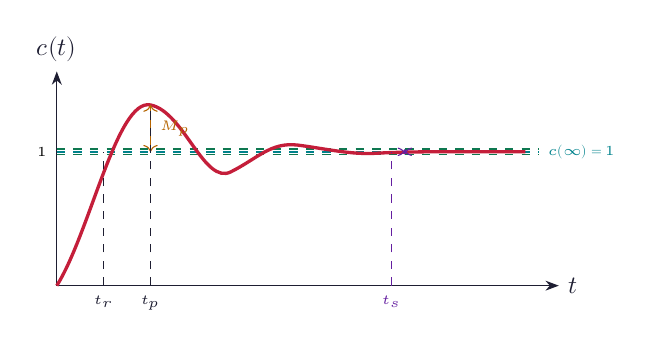
\begin{tikzpicture}[scale=0.85]
  % Axes
  \draw[axis] (0,0) -- (7.5,0) node[right,font=\small] {$t$};
  \draw[axis] (0,0) -- (0,3.2) node[above,font=\small] {$c(t)$};
  % Final value line
  \draw[dashed, color=myteal, line width=0.6pt] (0,2) -- (7.2,2) node[right,font=\tiny,color=myteal] {$c(\infty)=1$};
  % 2% band
  \draw[dashed, color=mygreen, line width=0.5pt] (0,2.04) -- (7.2,2.04);
  \draw[dashed, color=mygreen, line width=0.5pt] (0,1.96) -- (7.2,1.96);
  % Response curve (hand-drawn style)
  \draw[color=myred, line width=1.2pt]
    (0,0) .. controls (0.5,0.8) and (0.9,2.8) .. (1.4,2.7)
    .. controls (1.9,2.6) and (2.2,1.5) .. (2.6,1.7)
    .. controls (3.0,1.9) and (3.2,2.15) .. (3.6,2.1)
    .. controls (4.0,2.05) and (4.4,1.95) .. (4.8,1.98)
    .. controls (5.4,2.01) and (6.0,2.0) .. (7.0,2.0);
  % Annotations
  \draw[<->, color=myamber, thin] (1.4,2) -- (1.4,2.7) node[midway,right,font=\tiny,color=myamber] {$M_p$};
  \draw[dashed, color=mydark, thin] (1.4,0) node[below,font=\tiny] {$t_p$} -- (1.4,2.7);
  \draw[dashed, color=mydark, thin] (0.7,0) node[below,font=\tiny] {$t_r$} -- (0.7,2);
  \draw[<->, color=mypurple, thin] (5.2,1.96) -- (5.2,2.04);
  \draw[dashed, color=mypurple, thin] (5.0,0) node[below,font=\tiny,color=mypurple] {$t_s$} -- (5.0,2);
  \node at (0,2) [left,font=\tiny] {$1$};
\end{tikzpicture}
\end{tcolorbox}

%═══════════════════════════════════════════════════════════════════════════════
\section{Performance Specifications in Time Domain}
%═══════════════════════════════════════════════════════════════════════════════

Time-domain specifications quantify the transient and steady-state behaviour of a system's step response. They are used to set design requirements and evaluate controller performance.

\subsection{Transient Response Specifications}

\begin{tabularx}{\linewidth}{|B{3.0cm}|>{\centering\arraybackslash}p{2.2cm}|X|}
\hline
\multicolumn{1}{|>{\centering\arraybackslash}p{3.0cm}|}{\textbf{\color{myteal}Specification}} &
\multicolumn{1}{>{\centering\arraybackslash}p{2.2cm}|}{\textbf{\color{myteal}Symbol}} &
\multicolumn{1}{>{\centering\arraybackslash}X|}{\textbf{\color{myteal}Definition \& Formula}} \\
\hline
Rise Time & $t_r$ & Time for response to rise from 10\% to 90\% of final value (underdamped); or 0\% to 100\% (overdamped). $t_r \approx \dfrac{1.8}{\omega_n}$ \\
\hline
Peak Time & $t_p$ & Time to reach the first (maximum) peak of overshoot. $t_p = \dfrac{\pi}{\omega_d}$ \\
\hline
Peak Overshoot & $M_p$ & Maximum overshoot above final value, expressed as \%. $M_p = e^{-\pi\zeta/\sqrt{1-\zeta^2}} \times 100\%$ \\
\hline
Settling Time & $t_s$ & Time for response to stay within $\pm2\%$ (or $\pm5\%$) of final value. $t_s \approx \dfrac{4}{\zeta\omega_n}$ (2\% criterion) \\
\hline
Delay Time & $t_d$ & Time for response to reach 50\% of final value for the first time. $t_d \approx \dfrac{1+0.7\zeta}{\omega_n}$ \\
\hline
\end{tabularx}

\begin{tcolorbox}[formulabox, title={Key Relations — Underdamped 2nd Order}]
\begin{tabularx}{\linewidth}{>{\raggedright\arraybackslash}X >{\raggedright\arraybackslash}X}
$\omega_d = \omega_n\sqrt{1-\zeta^2}$ & Damped natural frequency \\[3pt]
$t_p = \pi/\omega_d$ & Peak time \\[3pt]
$M_p = e^{-\pi\zeta/\sqrt{1-\zeta^2}}\times100\%$ & \% Peak overshoot \\[3pt]
$t_s \approx 4/(\zeta\omega_n)$ & Settling time (2\% band) \\[3pt]
$t_s \approx 3/(\zeta\omega_n)$ & Settling time (5\% band) \\[3pt]
$\zeta = \cos\theta$ & $\theta$ = angle of pole from $-\sigma$ axis
\end{tabularx}
\end{tcolorbox}

\begin{tcolorbox}[exambox, title={Exam Tips — Time Domain Specs}]
\begin{itemize}[leftmargin=*, itemsep=3pt, topsep=0pt]
  \item \textbf{Higher $\omega_n$} → faster response (smaller $t_r$, $t_p$, $t_s$).
  \item \textbf{Higher $\zeta$} → less overshoot, more damping, slower rise.
  \item \textbf{$\zeta = 0.707$} gives $\approx 4.3\%$ overshoot — often used as optimal damping.
  \item \textbf{$M_p$ depends only on $\zeta$}; $t_p$ depends on $\omega_d$; $t_s$ depends on $\zeta\omega_n$.
  \item For a 2nd order system, poles at $s = -\zeta\omega_n \pm j\omega_d$ — draw on $s$-plane for viva.
\end{itemize}
\end{tcolorbox}

%═══════════════════════════════════════════════════════════════════════════════
\section{Steady-State Error and Error Constants}
%═══════════════════════════════════════════════════════════════════════════════

\begin{tcolorbox}[defbox]
\textbf{Steady-State Error:} The difference between the desired reference and the actual output as $t \to \infty$:
$$e_{ss} = \lim_{s \to 0}\, s\,E(s) = \lim_{s \to 0}\, \frac{s\,R(s)}{1 + G(s)H(s)}$$
Valid only when the closed-loop system is \textbf{stable} (Final Value Theorem condition).
\end{tcolorbox}

\subsection{Error Constants}

\begin{tcolorbox}[formulabox, title={Static Error Constants}]
$$K_p = \lim_{s\to 0} G(s)H(s) \quad \text{(Position — for step input)}$$
$$K_v = \lim_{s\to 0}\, s\,G(s)H(s) \quad \text{(Velocity — for ramp input)}$$
$$K_a = \lim_{s\to 0}\, s^2\,G(s)H(s) \quad \text{(Acceleration — for parabolic input)}$$
\end{tcolorbox}

\subsection{SSE vs System Type}

\begin{tabularx}{\linewidth}{|>{\centering\arraybackslash}X|>{\centering\arraybackslash}X|>{\centering\arraybackslash}X|>{\centering\arraybackslash}X|}
\hline
\textbf{\color{myteal}Input} & \textbf{\color{myteal}Type 0} & \textbf{\color{myteal}Type 1} & \textbf{\color{myteal}Type 2} \\
\hline
Step $\left(\frac{1}{s}\right)$         & $\dfrac{1}{1+K_p}$ & $0$              & $0$ \\
\hline
Ramp $\left(\frac{1}{s^2}\right)$       & $\infty$           & $\dfrac{1}{K_v}$ & $0$ \\
\hline
Parabola $\left(\frac{1}{s^3}\right)$   & $\infty$           & $\infty$         & $\dfrac{1}{K_a}$ \\
\hline
\end{tabularx}

\begin{tcolorbox}[exambox, title={Exam Tips — SSE}]
\begin{itemize}[leftmargin=*, itemsep=3pt, topsep=0pt]
  \item \textbf{System type} = number of open-loop poles at $s=0$ (pure integrators).
  \item Increasing gain $K$ reduces SSE but may reduce stability margin.
  \item Adding an integrator (increasing type) eliminates SSE for lower-order inputs.
  \item \textbf{FVT applies only if} $sE(s)$ has all poles in LHP — check stability first.
  \item For non-unity feedback: $e_{ss} = \lim_{s\to0} \dfrac{sR(s)}{1+G(s)H(s)}$.
\end{itemize}
\end{tcolorbox}

%═══════════════════════════════════════════════════════════════════════════════
\section{Root Locus Method}
%═══════════════════════════════════════════════════════════════════════════════

The \textbf{Root Locus} is a graphical method that shows how the closed-loop poles move in the $s$-plane as the open-loop gain $K$ varies from $0$ to $\infty$. It is the most powerful tool for \textbf{controller design} and \textbf{stability analysis}.

\begin{tcolorbox}[defbox]
\textbf{Definition:} The root locus is the locus (path) of the closed-loop poles of the system $T(s) = \dfrac{KG(s)}{1+KG(s)H(s)}$ as $K$ varies from $0$ to $+\infty$.\\[4pt]
\textbf{Characteristic equation:} $1 + KG(s)H(s) = 0 \;\Rightarrow\; G(s)H(s) = -\dfrac{1}{K}$\\[4pt]
\textbf{Angle condition:} $\angle G(s)H(s) = (2q+1)\cdot 180°$, $q = 0,\pm1,\pm2,\ldots$\\[2pt]
\textbf{Magnitude condition:} $|KG(s)H(s)| = 1$
\end{tcolorbox}

\subsection{Rules for Constructing Root Locus}

Let $G(s)H(s) = \dfrac{K\prod(s+z_i)}{\prod(s+p_j)}$ have $m$ zeros and $n$ poles ($n \geq m$).

\begin{tabularx}{\linewidth}{|>{\centering\arraybackslash}p{0.6cm}|B{3.4cm}|X|}
\hline
\multicolumn{1}{|>{\centering\arraybackslash}p{0.6cm}|}{\textbf{\color{myteal}\#}} &
\multicolumn{1}{>{\centering\arraybackslash}p{3.4cm}|}{\textbf{\color{myteal}Rule}} &
\multicolumn{1}{>{\centering\arraybackslash}X|}{\textbf{\color{myteal}Statement}} \\
\hline
1 & Number of branches & Equal to $n$ (number of open-loop poles). \\
\hline
2 & Start \& End points & Locus starts ($K=0$) at open-loop \textbf{poles}; ends ($K\to\infty$) at open-loop \textbf{zeros} (finite or at $\infty$). \\
\hline
3 & Symmetry & Root locus is always \textbf{symmetric about the real axis}. \\
\hline
4 & Real axis segments & A point on the real axis lies on the locus if the \textbf{total number of real poles and zeros to its right is odd}. \\
\hline
5 & Asymptotes & $(n-m)$ branches go to $\infty$ along asymptotes with angles: $\phi_k = \dfrac{(2k+1)\cdot180°}{n-m}$, $k=0,1,\ldots,(n-m-1)$ \\
\hline
6 & Centroid of asymptotes & $\sigma_a = \dfrac{\sum\text{poles} - \sum\text{zeros}}{n-m}$ (intersection of asymptotes on real axis) \\
\hline
7 & Breakaway / Break-in & Points where locus leaves/enters real axis. Found from $\dfrac{dK}{ds}=0$, i.e.\ $\dfrac{d}{ds}[G(s)H(s)]=0$. \\
\hline
8 & $j\omega$-axis crossing & Substitute $s=j\omega$ in characteristic equation; solve for $\omega$ and $K$. (Or use Routh array.) \\
\hline
9 & Angle of departure & From a complex pole $p_k$: $\phi_{dep} = 180° - \sum\angle(p_k - z_i) + \sum\angle(p_k - p_j)$ \\
\hline
10 & Angle of arrival & At a complex zero $z_k$: $\phi_{arr} = 180° + \sum\angle(z_k - p_j) - \sum\angle(z_k - z_i)$ \\
\hline
\end{tabularx}

\subsection{Root Locus — Worked Example}

\begin{tcolorbox}[examplebox, title={Example: $G(s)H(s) = K/[s(s+2)(s+4)]$}]
\textbf{Given:} $n=3$ poles at $s=0,-2,-4$; $m=0$ zeros.

\textbf{Step 1 — Branches:} 3 branches.

\textbf{Step 2 — Real axis segments:} Right of $s=0$: 0 poles/zeros → not on locus. Between $0$ and $-2$: 1 pole to right → \textbf{on locus}. Between $-2$ and $-4$: 2 poles to right → not on locus. Left of $-4$: 3 poles to right → \textbf{on locus}.

\textbf{Step 3 — Asymptotes:} $n-m=3$, angles $= 60°, 180°, 300°$.

\textbf{Step 4 — Centroid:} $\sigma_a = \dfrac{(0-2-4)-0}{3} = -2$.

\textbf{Step 5 — Breakaway:} $\dfrac{dK}{ds}=0 \Rightarrow 3s^2+12s+8=0 \Rightarrow s \approx -0.845$ (valid, between $0$ and $-2$).

\textbf{Step 6 — $j\omega$ crossing:} Characteristic eq: $s^3+6s^2+8s+K=0$. Routh: $K_{max}=48$, crossing at $\omega=\pm2\sqrt{2}$.
\end{tcolorbox}

\begin{tcolorbox}[tikzbox, title={Root Locus Sketch — $K/[s(s+2)(s+4)]$}]
\centering
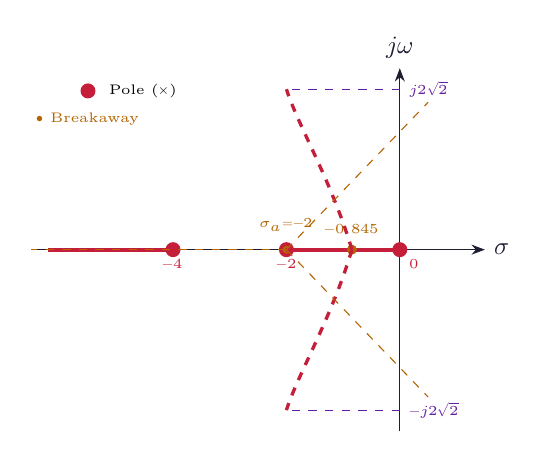
\begin{tikzpicture}[scale=0.72]
  % Axes
  \draw[axis] (-6.5,0) -- (1.5,0) node[right,font=\small] {$\sigma$};
  \draw[axis] (0,-3.2) -- (0,3.2) node[above,font=\small] {$j\omega$};
  % Poles
  \node[polenode] at (0,0) {};   \node[below right,font=\tiny,color=myred] at (0,0) {$0$};
  \node[polenode] at (-2,0) {};  \node[below,font=\tiny,color=myred] at (-2,0) {$-2$};
  \node[polenode] at (-4,0) {};  \node[below,font=\tiny,color=myred] at (-4,0) {$-4$};
  % Centroid
  \node[below,font=\tiny,color=myamber] at (-2,-0.15) {};
  \fill[myamber] (-2,0) circle (2pt);
  \node[above,font=\tiny,color=myamber] at (-2,0.15) {$\sigma_a{=}{-2}$};
  % Real axis locus
  \draw[color=myred, line width=1.4pt] (0,0) -- (-2,0);
  \draw[color=myred, line width=1.4pt] (-4,0) -- (-6.2,0);
  % Breakaway
  \fill[myamber] (-0.845,0) circle (2.5pt);
  \node[above,font=\tiny,color=myamber] at (-0.845,0.1) {$-0.845$};
  % Complex branches (approximate)
  \draw[color=myred, line width=1.2pt, dashed]
    (-0.845,0) .. controls (-1.2,1.2) and (-1.8,2.2) .. (-2,2.83);
  \draw[color=myred, line width=1.2pt, dashed]
    (-0.845,0) .. controls (-1.2,-1.2) and (-1.8,-2.2) .. (-2,-2.83);
  % Asymptote lines (60 deg from centroid)
  \draw[color=myamber, thin, dashed] (-2,0) -- (0.5,2.6);
  \draw[color=myamber, thin, dashed] (-2,0) -- (-6.5,0);
  \draw[color=myamber, thin, dashed] (-2,0) -- (0.5,-2.6);
  % jw crossing
  \draw[dashed, color=mypurple, thin] (0,2.83) node[right,font=\tiny,color=mypurple] {$j2\sqrt{2}$} -- (-2,2.83);
  \draw[dashed, color=mypurple, thin] (0,-2.83) node[right,font=\tiny,color=mypurple] {$-j2\sqrt{2}$} -- (-2,-2.83);
  % Legend
  \node[polenode] at (-5.5,2.8) {}; \node[right,font=\tiny] at (-5.3,2.8) {Pole ($\times$)};
  \node[font=\tiny,color=myamber] at (-5.5,2.3) {$\bullet$ Breakaway};
\end{tikzpicture}
\end{tcolorbox}

\begin{tcolorbox}[exambox, title={Exam Tips — Root Locus}]
\begin{itemize}[leftmargin=*, itemsep=3pt, topsep=0pt]
  \item \textbf{Locus starts at poles, ends at zeros} — memorise this first.
  \item \textbf{Real axis rule:} odd number of poles+zeros to the right → on locus.
  \item \textbf{Centroid formula:} $\sigma_a = (\sum p_i - \sum z_i)/(n-m)$ — very frequently asked.
  \item \textbf{Breakaway point:} solve $dK/ds = 0$ or equivalently $d[G(s)H(s)]/ds = 0$.
  \item \textbf{$j\omega$ crossing:} use Routh array or substitute $s=j\omega$ — gives $K_{max}$ for stability.
  \item \textbf{Gain $K$} at any point on locus: $K = 1/|G(s)H(s)|$ at that $s$.
\end{itemize}
\end{tcolorbox}

%═══════════════════════════════════════════════════════════════════════════════
\section{Compensator Design}
%═══════════════════════════════════════════════════════════════════════════════

A \textbf{compensator} (or controller) is added to the forward or feedback path to reshape the root locus so that the closed-loop poles are placed at desired locations, meeting the time-domain specifications.

\begin{tcolorbox}[defbox]
\textbf{Compensator:} A dynamic element $G_c(s)$ inserted in the control loop to improve transient response, steady-state accuracy, or both. The two fundamental types are \textbf{Lead} (improves transient) and \textbf{Lag} (improves steady-state).
\end{tcolorbox}

%───────────────────────────────────────────────────────────────────────────────
\subsection{Lead Compensator}
%───────────────────────────────────────────────────────────────────────────────

\begin{tcolorbox}[defbox]
\textbf{Lead Compensator:} A compensator whose \textbf{zero is closer to the origin than its pole}. It adds a net \textit{positive} phase angle to the open-loop transfer function, effectively acting like a \textbf{PD controller}. It improves \textbf{transient response} — faster rise time, reduced overshoot.
\end{tcolorbox}

\begin{tcolorbox}[formulabox, title={Lead Compensator Transfer Function}]
$$G_c(s) = K_c\,\frac{s + z_c}{s + p_c}, \qquad p_c > z_c > 0 \quad (\text{pole farther from origin than zero})$$
\textbf{Phase contribution:} $\phi = \angle(s+z_c) - \angle(s+p_c) > 0$ \quad (positive phase lead)\\[4pt]
\textbf{Maximum phase lead:} $\phi_{max} = \sin^{-1}\!\left(\dfrac{1-\alpha}{1+\alpha}\right)$, where $\alpha = z_c/p_c < 1$\\[4pt]
\textbf{Frequency of max lead:} $\omega_{max} = \sqrt{z_c \cdot p_c}$
\end{tcolorbox}

\subsubsection*{Op-Amp Realization of Lead Compensator}

\begin{tcolorbox}[tikzbox, title={Lead Network (RC Circuit)}]
\centering
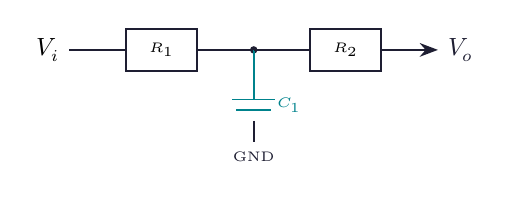
\begin{tikzpicture}[scale=0.9, font=\small]
  % Input
  \draw[line width=0.7pt,color=mydark] (0,1.8) -- (0.8,1.8);
  % R1
  \draw[line width=0.7pt,color=mydark] (0.8,1.5) rectangle (1.8,2.1);
  \node at (1.3,1.8) [font=\tiny] {$R_1$};
  \draw[line width=0.7pt,color=mydark] (1.8,1.8) -- (2.6,1.8);
  % Junction
  \fill[mydark] (2.6,1.8) circle (1.5pt);
  % C1 to ground
  \draw[line width=0.7pt,color=myteal] (2.6,1.8) -- (2.6,1.1);
  \draw[line width=0.7pt,color=myteal] (2.3,1.1) -- (2.9,1.1);
  \draw[line width=0.7pt,color=myteal] (2.35,0.95) -- (2.85,0.95);
  \node at (3.1,1.02) [font=\tiny,color=myteal] {$C_1$};
  \draw[line width=0.7pt,color=mydark] (2.6,0.8) -- (2.6,0.5) node[below,font=\tiny] {GND};
  % R2
  \draw[line width=0.7pt,color=mydark] (2.6,1.8) -- (3.4,1.8);
  \draw[line width=0.7pt,color=mydark] (3.4,1.5) rectangle (4.4,2.1);
  \node at (3.9,1.8) [font=\tiny] {$R_2$};
  \draw[arrow] (4.4,1.8) -- (5.2,1.8) node[right,font=\small] {$V_o$};
  \node at (-0.3,1.8) [font=\small] {$V_i$};
\end{tikzpicture}

\vspace{4pt}
\centering
{\small\color{myteal}$G_c(s)=\dfrac{R_2}{R_1+R_2}\cdot\dfrac{1+sR_1C_1}{1+s\dfrac{R_1R_2}{R_1+R_2}C_1}$}
\end{tcolorbox}

\subsubsection*{Design Procedure (Root Locus)}

\begin{enumerate}[label=\textbf{Step \arabic*:}, leftmargin=2.5cm, itemsep=3pt]
  \item Determine desired closed-loop pole location $s_d$ from specs ($M_p$, $t_s$, $t_p$).
  \item Calculate the \textbf{angle deficiency}: $\phi = 180° - \angle G(s_d)H(s_d)$.
  \item Place the compensator zero $z_c$ and pole $p_c$ such that they contribute angle $\phi$ at $s_d$.
  \item Determine gain $K_c$ from the magnitude condition: $K_c = 1/|G_c(s_d)G(s_d)H(s_d)|$.
  \item Verify SSE and adjust if needed.
\end{enumerate}

%───────────────────────────────────────────────────────────────────────────────
\subsection{Lag Compensator}
%───────────────────────────────────────────────────────────────────────────────

\begin{tcolorbox}[defbox]
\textbf{Lag Compensator:} A compensator whose \textbf{pole is closer to the origin than its zero}. It adds a net \textit{negative} phase angle (phase lag), effectively acting like a \textbf{PI controller}. It improves \textbf{steady-state accuracy} (increases low-frequency gain) without significantly altering the transient response.
\end{tcolorbox}

\begin{tcolorbox}[formulabox, title={Lag Compensator Transfer Function}]
$$G_c(s) = K_c\,\frac{s + z_c}{s + p_c}, \qquad 0 < p_c < z_c \quad (\text{zero farther from origin than pole})$$
\textbf{DC gain boost:} $G_c(0) = K_c\,\dfrac{z_c}{p_c} = K_c\,\beta$, where $\beta = z_c/p_c > 1$\\[4pt]
The lag compensator increases the \textbf{velocity constant} $K_v$ by a factor of $\beta$, reducing SSE.\\[4pt]
\textbf{Placement rule:} Place $z_c$ and $p_c$ very close to the origin (e.g., $z_c = 0.1$, $p_c = 0.01$) so they do not disturb the root locus significantly.
\end{tcolorbox}

\subsubsection*{Op-Amp Realization of Lag Compensator}

\begin{tcolorbox}[tikzbox, title={Lag Network (RC Circuit)}]
\centering
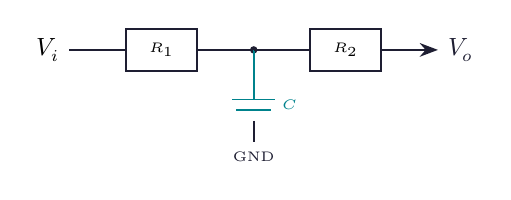
\begin{tikzpicture}[scale=0.9, font=\small]
  % Input wire
  \draw[line width=0.7pt,color=mydark] (0,1.8) -- (0.8,1.8);
  % R1
  \draw[line width=0.7pt,color=mydark] (0.8,1.5) rectangle (1.8,2.1);
  \node at (1.3,1.8) [font=\tiny] {$R_1$};
  \draw[line width=0.7pt,color=mydark] (1.8,1.8) -- (2.6,1.8);
  \fill[mydark] (2.6,1.8) circle (1.5pt);
  % C to ground (below junction)
  \draw[line width=0.7pt,color=myteal] (2.6,1.8) -- (2.6,1.1);
  \draw[line width=0.7pt,color=myteal] (2.3,1.1) -- (2.9,1.1);
  \draw[line width=0.7pt,color=myteal] (2.35,0.95) -- (2.85,0.95);
  \node at (3.1,1.02) [font=\tiny,color=myteal] {$C$};
  \draw[line width=0.7pt,color=mydark] (2.6,0.8) -- (2.6,0.5) node[below,font=\tiny] {GND};
  % R2
  \draw[line width=0.7pt,color=mydark] (2.6,1.8) -- (3.4,1.8);
  \draw[line width=0.7pt,color=mydark] (3.4,1.5) rectangle (4.4,2.1);
  \node at (3.9,1.8) [font=\tiny] {$R_2$};
  \draw[arrow] (4.4,1.8) -- (5.2,1.8) node[right,font=\small] {$V_o$};
  % Input label
  \node at (-0.3,1.8) [font=\small] {$V_i$};
\end{tikzpicture}

\vspace{4pt}
\centering
{\small\color{myteal}$G_c(s)=\dfrac{1+sR_2C}{1+s(R_1+R_2)C}$, \quad pole $<$ zero}
\end{tcolorbox}

\subsubsection*{Design Procedure (Root Locus)}

\begin{enumerate}[label=\textbf{Step \arabic*:}, leftmargin=2.5cm, itemsep=3pt]
  \item Design the uncompensated system to meet transient specs (find required $K$).
  \item Determine the factor $\beta = z_c/p_c$ needed to achieve the desired SSE improvement.
  \item Place $z_c$ and $p_c$ near the origin (e.g., $z_c = 0.1$, $p_c = z_c/\beta$).
  \item Verify that the lag compensator does not significantly shift the dominant poles.
  \item Recalculate gain $K_c$ from magnitude condition at the desired pole.
\end{enumerate}

%───────────────────────────────────────────────────────────────────────────────
\subsection{Lead vs Lag — Comparison}
%───────────────────────────────────────────────────────────────────────────────

\begin{tabularx}{\linewidth}{|B{3.2cm}|>{\centering\arraybackslash}X|>{\centering\arraybackslash}X|}
\hline
\multicolumn{1}{|>{\centering\arraybackslash}p{3.2cm}|}{\textbf{Property}} &
\textbf{\color{myred}Lead Compensator} & \textbf{\color{mygreen}Lag Compensator} \\
\hline
Pole-zero relation & $p_c > z_c$ (pole farther) & $p_c < z_c$ (pole closer) \\
\hline
Phase contribution & Positive (phase lead) & Negative (phase lag) \\
\hline
Equivalent to & PD controller & PI controller \\
\hline
Primary effect & Improves transient response & Improves steady-state accuracy \\
\hline
Bandwidth & Increases & Decreases slightly \\
\hline
Noise sensitivity & Higher (differentiating action) & Lower \\
\hline
Root locus effect & Shifts locus to the left (more stable) & Provides gain boost near origin \\
\hline
Typical use & Fast response needed & Low SSE needed without changing transient \\
\hline
\end{tabularx}

\subsection{Lead-Lag Compensator}

\begin{tcolorbox}[defbox]
\textbf{Lead-Lag Compensator:} Combines both lead and lag sections in cascade to simultaneously improve transient response \textit{and} steady-state accuracy:
$$G_c(s) = K_c\,\frac{(s+z_1)(s+z_2)}{(s+p_1)(s+p_2)}, \quad p_1 > z_1 \text{ (lead)}, \quad p_2 < z_2 \text{ (lag)}$$
Equivalent to a \textbf{PID controller} in terms of effect.
\end{tcolorbox}

\begin{tcolorbox}[exambox, title={Exam Tips — Compensators}]
\begin{itemize}[leftmargin=*, itemsep=3pt, topsep=0pt]
  \item \textbf{Lead:} zero closer to origin than pole → phase lead → faster response.
  \item \textbf{Lag:} pole closer to origin than zero → phase lag → better SSE.
  \item \textbf{Angle deficiency} = $180° - \angle G(s_d)H(s_d)$ — must be provided by lead compensator.
  \item \textbf{$\beta$ factor} for lag = ratio $z_c/p_c$ = SSE improvement factor.
  \item Lead-lag = PID equivalent; used when both transient and SSE specs must be met.
  \item \textbf{RC lead network:} $G_c(s) \propto (1+sR_1C)/(1+s\frac{R_1R_2}{R_1+R_2}C)$ — pole $>$ zero.
  \item \textbf{RC lag network:} $G_c(s) \propto (1+sR_2C)/(1+s(R_1+R_2)C)$ — pole $<$ zero.
\end{itemize}
\end{tcolorbox}

%═══════════════════════════════════════════════════════════════════════════════
% QUICK REVISION — MODULE 3
%═══════════════════════════════════════════════════════════════════════════════
\newpage
\begin{center}
  {\large\bfseries\color{myred} Quick Revision — Module 3}\\[3pt]
  {\small\color{mydark} Time Response, Root Locus \& Compensators $|$ EC601}
\end{center}
\noindent{\color{myred}\rule{\linewidth}{1.2pt}}
\vspace{4pt}

\begin{tcolorbox}[formulabox, title={\textbf{Key Formulas at a Glance}}]
\begin{tabularx}{\linewidth}{B{5.0cm} X}
Standard 2nd order TF      & $G(s) = \omega_n^2/(s^2+2\zeta\omega_n s+\omega_n^2)$ \\[2pt]
Poles                      & $s_{1,2} = -\zeta\omega_n \pm j\omega_d$ \\[2pt]
Damped freq.               & $\omega_d = \omega_n\sqrt{1-\zeta^2}$ \\[2pt]
Peak time                  & $t_p = \pi/\omega_d$ \\[2pt]
\% Peak overshoot          & $M_p = e^{-\pi\zeta/\sqrt{1-\zeta^2}}\times100\%$ \\[2pt]
Settling time (2\%)        & $t_s \approx 4/(\zeta\omega_n)$ \\[2pt]
Settling time (5\%)        & $t_s \approx 3/(\zeta\omega_n)$ \\[2pt]
Rise time (approx.)        & $t_r \approx 1.8/\omega_n$ \\[2pt]
SSE (step, Type 0)         & $1/(1+K_p)$ \\[2pt]
SSE (ramp, Type 1)         & $1/K_v$ \\[2pt]
Asymptote angles           & $\phi_k = (2k+1)\cdot180°/(n-m)$ \\[2pt]
Centroid                   & $\sigma_a = (\sum p_i - \sum z_i)/(n-m)$ \\[2pt]
Gain at point $s_d$        & $K = 1/|G(s_d)H(s_d)|$ \\[2pt]
Lead TF                    & $K_c(s+z_c)/(s+p_c)$, $p_c>z_c$ \\[2pt]
Lag TF                     & $K_c(s+z_c)/(s+p_c)$, $p_c<z_c$ \\[2pt]
Max phase lead             & $\phi_{max}=\sin^{-1}[(1-\alpha)/(1+\alpha)]$, $\alpha=z_c/p_c$
\end{tabularx}
\end{tcolorbox}

\vspace{5pt}

\begin{tcolorbox}[defbox, title={\textbf{One-Line Definitions}}]
\begin{itemize}[leftmargin=*, itemsep=3pt, topsep=0pt]
  \item \textbf{$\omega_n$:} Natural frequency — speed of oscillation without damping.
  \item \textbf{$\zeta$:} Damping ratio — controls oscillation; $\zeta=1$ is critically damped.
  \item \textbf{$\omega_d$:} Damped natural frequency — actual oscillation frequency in underdamped response.
  \item \textbf{Rise time $t_r$:} Time to go from 10\% to 90\% of final value.
  \item \textbf{Peak time $t_p$:} Time to reach first overshoot peak; $t_p = \pi/\omega_d$.
  \item \textbf{Overshoot $M_p$:} Maximum exceedance above final value; depends only on $\zeta$.
  \item \textbf{Settling time $t_s$:} Time to stay within $\pm2\%$ band; $t_s \approx 4/(\zeta\omega_n)$.
  \item \textbf{Root locus:} Path of closed-loop poles as gain $K$ varies $0\to\infty$.
  \item \textbf{Breakaway point:} Point where locus leaves real axis; found from $dK/ds=0$.
  \item \textbf{Centroid:} Intersection of asymptotes on real axis; $\sigma_a = (\sum p - \sum z)/(n-m)$.
  \item \textbf{Lead compensator:} Adds phase lead; improves transient; pole farther than zero.
  \item \textbf{Lag compensator:} Adds phase lag; improves SSE; pole closer than zero.
  \item \textbf{Angle deficiency:} Phase that lead compensator must supply at desired pole location.
\end{itemize}
\end{tcolorbox}

\vspace{5pt}

\begin{tcolorbox}[exambox, title={\textbf{Frequently Asked / Viva Questions}}]
\begin{enumerate}[leftmargin=*, topsep=0pt, label=\textbf{Q\arabic*.}, itemsep=8pt]
  \item \Q{What is the standard second-order transfer function?} $G(s) = \omega_n^2/(s^2+2\zeta\omega_n s+\omega_n^2)$.
  \item \Q{What is the effect of $\zeta$ on step response?} $\zeta<1$: underdamped (oscillatory); $\zeta=1$: critically damped (fastest non-oscillatory); $\zeta>1$: overdamped (sluggish).
  \item \Q{How is $M_p$ related to $\zeta$?} $M_p = e^{-\pi\zeta/\sqrt{1-\zeta^2}}\times100\%$ — depends only on $\zeta$, not $\omega_n$.
  \item \Q{What is the 2\% settling time formula?} $t_s \approx 4/(\zeta\omega_n)$.
  \item \Q{What does the root locus start and end at?} Starts at open-loop poles ($K=0$), ends at open-loop zeros ($K\to\infty$).
  \item \Q{State the real axis rule for root locus.} A point on the real axis is on the locus if the total number of real poles and zeros to its right is odd.
  \item \Q{What is the centroid formula?} $\sigma_a = (\sum\text{poles} - \sum\text{zeros})/(n-m)$.
  \item \Q{How do you find the breakaway point?} Differentiate $K = -1/G(s)H(s)$ with respect to $s$ and set to zero; or solve $d[G(s)H(s)]/ds = 0$.
  \item \Q{What is the difference between lead and lag compensator?} Lead: $p>z$, adds positive phase, improves transient. Lag: $p<z$, adds negative phase, improves SSE.
  \item \Q{What is angle deficiency?} The phase angle that the lead compensator must contribute at the desired closed-loop pole location: $\phi = 180° - \angle G(s_d)H(s_d)$.
  \item \Q{What is the $\beta$ factor in lag compensator?} $\beta = z_c/p_c > 1$; it is the factor by which the velocity constant $K_v$ (and hence SSE improvement) is multiplied.
  \item \Q{What is a lead-lag compensator equivalent to?} A PID controller — provides both transient improvement (lead) and SSE improvement (lag).
\end{enumerate}
\end{tcolorbox}

\vspace{5pt}

\begin{tcolorbox}[tikzbox, title={\textbf{Damping Cases — Quick Reference}}]
\begin{tabularx}{\linewidth}{|>{\centering\arraybackslash}X|>{\centering\arraybackslash}X|>{\centering\arraybackslash}X|}
\hline
\textbf{\color{myteal}$\zeta$ value} & \textbf{\color{myteal}Pole type} & \textbf{\color{myteal}Response} \\
\hline
$\zeta = 0$ & $\pm j\omega_n$ & Undamped — sustained oscillation \\
\hline
$0 < \zeta < 1$ & Complex conjugate & Underdamped — decaying oscillation \\
\hline
$\zeta = 1$ & Two equal real & Critically damped — fastest non-oscillatory \\
\hline
$\zeta > 1$ & Two distinct real & Overdamped — no oscillation, slow \\
\hline
\end{tabularx}
\end{tcolorbox}

\vspace{5pt}

\begin{tcolorbox}[tikzbox, title={\textbf{Root Locus Rules — Quick Reference}}]
\begin{tabularx}{\linewidth}{|>{\centering\arraybackslash}p{0.5cm}|B{3.2cm}|X|}
\hline
\textbf{\color{myteal}\#} & \multicolumn{1}{>{\centering\arraybackslash}p{3.2cm}|}{\textbf{\color{myteal}Rule}} & \multicolumn{1}{>{\centering\arraybackslash}X|}{\textbf{\color{myteal}Formula / Statement}} \\
\hline
1 & Branches & $n$ branches (= no.\ of poles) \\
\hline
2 & Start/End & $K=0$: poles; $K\to\infty$: zeros \\
\hline
3 & Symmetry & Symmetric about real axis \\
\hline
4 & Real axis & Odd poles+zeros to the right \\
\hline
5 & Asymptote angles & $(2k+1)\cdot180°/(n-m)$ \\
\hline
6 & Centroid & $(\sum p_i - \sum z_i)/(n-m)$ \\
\hline
7 & Breakaway & $dK/ds = 0$ \\
\hline
8 & $j\omega$ crossing & $s=j\omega$ in char.\ eq.\ or Routh \\
\hline
\end{tabularx}
\end{tcolorbox}


% -- Module 4 -----------------------------------------------------------------
\modulestart{4}{Frequency Response Analysis --- Introduction}

\section{Frequency Response Analysis --- Introduction}
%═══════════════════════════════════════════════════════════════════════════════

\textbf{Frequency response analysis} studies how a system responds to sinusoidal inputs of varying frequency. For a stable LTI system with transfer function $G(j\omega)$, a sinusoidal input $r(t)=A\sin(\omega t)$ produces a steady-state output $c(t)=A|G(j\omega)|\sin(\omega t + \angle G(j\omega))$.

\begin{tcolorbox}[defbox]
\textbf{Frequency Response Function:} Obtained by substituting $s = j\omega$ in the transfer function:
$$G(j\omega) = G(s)\big|_{s=j\omega} = |G(j\omega)|\,\angle\phi(\omega)$$
\textbf{Magnitude:} $|G(j\omega)|$ --- ratio of output to input amplitude.\\
\textbf{Phase:} $\phi(\omega) = \angle G(j\omega)$ --- phase shift of output relative to input.
\end{tcolorbox}

\begin{tabularx}{\linewidth}{|B{3.2cm}|X|}
\hline
\multicolumn{1}{|>{\centering\arraybackslash}p{3.2cm}|}{\textbf{\color{myteal}Plot Type}} &
\multicolumn{1}{>{\centering\arraybackslash}X|}{\textbf{\color{myteal}Description}} \\
\hline
Polar Plot & Locus of $G(j\omega)$ in the complex plane as $\omega: 0\to\infty$. Also called Nyquist plot (open-loop). \\
\hline
Bode Plot & Two separate plots: $|G(j\omega)|$ in dB vs $\log\omega$, and $\angle G(j\omega)$ in degrees vs $\log\omega$. \\
\hline
Nyquist Plot & Polar plot of $G(j\omega)H(j\omega)$ for $\omega: -\infty\to+\infty$; used for Nyquist stability criterion. \\
\hline
Nichols Chart & Magnitude vs phase plot; used for closed-loop frequency response from open-loop data. \\
\hline
\end{tabularx}

%═══════════════════════════════════════════════════════════════════════════════
\section{Polar Plots}
%═══════════════════════════════════════════════════════════════════════════════

\begin{tcolorbox}[defbox]
\textbf{Polar Plot:} A plot of $G(j\omega)$ in the complex ($\text{Re}$--$\text{Im}$) plane as $\omega$ varies from $0$ to $+\infty$. Each point on the curve represents the tip of the phasor $G(j\omega)$ at a particular frequency. The distance from the origin is $|G(j\omega)|$ and the angle is $\angle G(j\omega)$.
\end{tcolorbox}

\subsection{Polar Plot of Standard Factors}

\begin{tabularx}{\linewidth}{|B{3.4cm}|>{\centering\arraybackslash}X|>{\centering\arraybackslash}X|}
\hline
\multicolumn{1}{|>{\centering\arraybackslash}p{3.4cm}|}{\textbf{\color{myteal}Factor}} &
\textbf{\color{myteal}At $\omega=0$} & \textbf{\color{myteal}At $\omega\to\infty$} \\
\hline
$K$ (gain) & $(K, 0°)$ & $(K, 0°)$ --- point on real axis \\
\hline
$j\omega$ (integrator) & $\infty\angle{-90°}$ & $0\angle{-90°}$ --- negative imaginary axis \\
\hline
$1/j\omega$ & $\infty\angle{-90°}$ & $0\angle{-90°}$ --- negative imaginary axis \\
\hline
$1/(1+j\omega T)$ & $(1, 0°)$ & $(0, -90°)$ --- 4th quadrant semicircle \\
\hline
$1/(j\omega)^2$ & $\infty\angle{-180°}$ & $0\angle{-180°}$ --- negative real axis \\
\hline
$1/[j\omega(1+j\omega T)]$ & $\infty\angle{-90°}$ & $0\angle{-180°}$ --- 3rd quadrant \\
\hline
\end{tabularx}

\subsection{Key Properties of Polar Plots}

\begin{itemize}[leftmargin=*, itemsep=3pt]
  \item The \textbf{starting point} ($\omega=0$) and \textbf{ending point} ($\omega\to\infty$) are determined by the system type and order.
  \item For a \textbf{Type 0} system: starts on positive real axis; for \textbf{Type 1}: starts at $-90°$ infinity; for \textbf{Type 2}: starts at $-180°$ infinity.
  \item The \textbf{number of clockwise encirclements} of the $(-1, j0)$ point determines closed-loop stability (Nyquist criterion).
  \item The \textbf{gain crossover frequency} $\omega_{gc}$: where $|G(j\omega)|=1$ (0 dB).
  \item The \textbf{phase crossover frequency} $\omega_{pc}$: where $\angle G(j\omega) = -180°$.
\end{itemize}

\begin{tcolorbox}[tikzbox, title={Polar Plot --- Type 1, Second Order: $G(j\omega)=K/[j\omega(1+j\omega T)]$}]
\centering
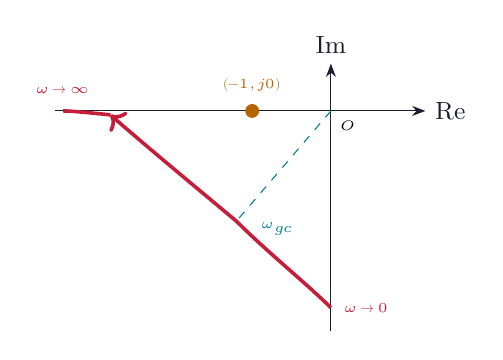
\begin{tikzpicture}[scale=1.0]
  % Axes
  \draw[axis] (-3.5,0) -- (1.2,0) node[right,font=\small] {Re};
  \draw[axis] (0,-2.8) -- (0,0.6) node[above,font=\small] {Im};
  % Curve: starts at -90 deg infinity, sweeps to origin at -180 deg
  \draw[color=myred, line width=1.3pt, ->]
    (0,-2.5) .. controls (-0.3,-2.2) and (-0.8,-1.8) .. (-1.2,-1.4)
    .. controls (-1.8,-0.9) and (-2.4,-0.4) .. (-2.8,-0.05);
  \draw[color=myred, line width=1.3pt]
    (-2.8,-0.05) .. controls (-3.1,-0.02) and (-3.3,0) .. (-3.4,0);
  % Labels
  \node[right, font=\tiny, color=myred] at (0.05,-2.5) {$\omega\to 0$};
  \node[above, font=\tiny, color=myred] at (-3.4,0.1) {$\omega\to\infty$};
  % -1,0 point
  \fill[myamber] (-1,0) circle (2.5pt);
  \node[above, font=\tiny, color=myamber] at (-1,0.12) {$(-1,j0)$};
  % Gain crossover
  \draw[dashed, color=myteal, thin] (0,0) -- (-1.2,-1.4);
  \node[right, font=\tiny, color=myteal] at (-1.0,-1.5) {$\omega_{gc}$};
  % Origin
  \node[below right, font=\tiny] at (0,0) {$O$};
\end{tikzpicture}
\end{tcolorbox}

%═══════════════════════════════════════════════════════════════════════════════
\section{Bode Plot}
%═══════════════════════════════════════════════════════════════════════════════

\begin{tcolorbox}[defbox]
\textbf{Bode Plot:} Two semi-log plots of the open-loop frequency response $G(j\omega)$:
\begin{itemize}[leftmargin=*, itemsep=2pt, topsep=2pt]
  \item \textbf{Magnitude plot:} $20\log_{10}|G(j\omega)|$ in \textbf{dB} vs $\log_{10}\omega$ (log scale).
  \item \textbf{Phase plot:} $\angle G(j\omega)$ in \textbf{degrees} vs $\log_{10}\omega$ (log scale).
\end{itemize}
Bode plots use \textbf{asymptotic approximations} (straight-line segments) for quick sketching.
\end{tcolorbox}

\subsection{Standard Factors and Their Bode Contributions}

\begin{tabularx}{\linewidth}{|B{3.0cm}|>{\centering\arraybackslash}X|>{\centering\arraybackslash}X|}
\hline
\multicolumn{1}{|>{\centering\arraybackslash}p{3.0cm}|}{\textbf{\color{myteal}Factor}} &
\textbf{\color{myteal}Magnitude (dB)} & \textbf{\color{myteal}Phase} \\
\hline
Gain $K$ & $20\log K$ (constant) & $0°$ (if $K>0$); $-180°$ (if $K<0$) \\
\hline
$j\omega$ (zero at origin) & $+20$ dB/dec, passes through 0 dB at $\omega=1$ & $+90°$ (constant) \\
\hline
$1/j\omega$ (pole at origin) & $-20$ dB/dec, passes through 0 dB at $\omega=1$ & $-90°$ (constant) \\
\hline
$(1+j\omega T)$ (simple zero) & $0$ dB for $\omega\ll1/T$; $+20$ dB/dec for $\omega\gg1/T$ & $0°\to+90°$, $45°$ at $\omega=1/T$ \\
\hline
$1/(1+j\omega T)$ (simple pole) & $0$ dB for $\omega\ll1/T$; $-20$ dB/dec for $\omega\gg1/T$ & $0°\to-90°$, $-45°$ at $\omega=1/T$ \\
\hline
$1/(j\omega)^2$ (double pole) & $-40$ dB/dec & $-180°$ (constant) \\
\hline
2nd order factor & $0$ dB below $\omega_n$; $-40$ dB/dec above $\omega_n$; resonance peak near $\omega_n$ & $0°\to-180°$, $-90°$ at $\omega_n$ \\
\hline
\end{tabularx}

\subsection{Corner Frequency (Break Frequency)}

\begin{tcolorbox}[formulabox, title={Corner Frequency}]
For a factor $(1+j\omega T)$: \textbf{corner frequency} $\omega_c = 1/T$ rad/s.\\[4pt]
\textbf{Asymptotic error at corner frequency:}
\begin{itemize}[leftmargin=*, itemsep=2pt, topsep=2pt]
  \item Magnitude: actual value differs from asymptote by $\pm 3$ dB at $\omega = \omega_c$.
  \item Phase: actual $= \pm 45°$ at $\omega_c$; asymptote approximation has $\pm 5.7°$ max error.
\end{itemize}
\end{tcolorbox}

\subsection{Bode Plot Sketching Procedure}

\begin{enumerate}[label=\textbf{Step \arabic*:}, leftmargin=2.5cm, itemsep=3pt]
  \item Write $G(j\omega)$ in \textbf{time-constant form}: factor out constants, express each factor as $(1+j\omega T)$.
  \item Compute the \textbf{initial slope}: $-20N$ dB/dec where $N$ = system type (number of poles at origin).
  \item Mark all \textbf{corner frequencies} $\omega_c = 1/T$ on the $\omega$-axis.
  \item Draw the \textbf{magnitude asymptotes}: slope changes by $+20$ dB/dec at each zero corner, $-20$ dB/dec at each pole corner.
  \item Apply \textbf{3 dB corrections} at each corner frequency if accuracy is needed.
  \item Draw the \textbf{phase plot}: sum contributions from each factor; use $\pm45°$/decade approximation.
\end{enumerate}

\begin{tcolorbox}[examplebox, title={Example: $G(j\omega) = \dfrac{10}{j\omega(1+0.1j\omega)(1+0.5j\omega)}$}]
\textbf{Factors:} Gain $K=10$ ($+20$ dB), pole at origin ($-20$ dB/dec from start), poles at $\omega_c=10$ and $\omega_c=2$.

\textbf{Initial value:} At $\omega=1$: $20\log(10/1) = 20$ dB (from gain and pole at origin).

\textbf{Slope changes:}
\begin{itemize}[leftmargin=*, itemsep=1pt, topsep=0pt]
  \item $\omega < 2$: slope $= -20$ dB/dec (one pole at origin)
  \item $2 < \omega < 10$: slope $= -40$ dB/dec (pole at $\omega=2$ adds $-20$)
  \item $\omega > 10$: slope $= -60$ dB/dec (pole at $\omega=10$ adds another $-20$)
\end{itemize}

\textbf{Phase:} $-90°$ (pole at origin) $-\tan^{-1}(0.5\omega) - \tan^{-1}(0.1\omega)$
\end{tcolorbox}

\begin{tcolorbox}[tikzbox, title={Bode Magnitude Plot Sketch}]
\centering
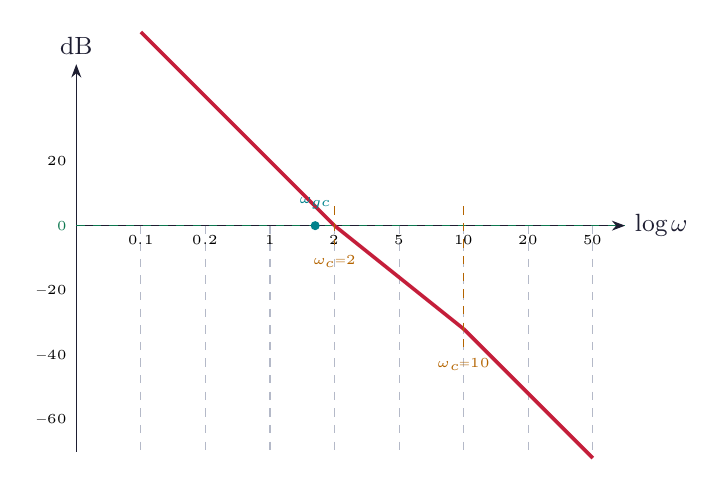
\begin{tikzpicture}[scale=0.82]
  % Axes
  \draw[axis] (0,0) -- (8.5,0) node[right,font=\small] {$\log\omega$};
  \draw[axis] (0,-3.5) -- (0,2.5) node[above,font=\small] {dB};
  % Grid lines
  \foreach \x in {1,2,3,4,5,6,7,8} \draw[gridline] (\x,0) -- (\x,-3.5);
  % Frequency labels
  \node[below,font=\tiny] at (1,0) {$0.1$};
  \node[below,font=\tiny] at (2,0) {$0.2$};
  \node[below,font=\tiny] at (3,0) {$1$};
  \node[below,font=\tiny] at (4,0) {$2$};
  \node[below,font=\tiny] at (5,0) {$5$};
  \node[below,font=\tiny] at (6,0) {$10$};
  \node[below,font=\tiny] at (7,0) {$20$};
  \node[below,font=\tiny] at (8,0) {$50$};
  % 0 dB line
  \draw[dashed, color=mygreen, thin] (0,0) -- (8.5,0);
  \node[left,font=\tiny,color=mygreen] at (0,0) {$0$};
  \node[left,font=\tiny] at (0,1) {$20$};
  \node[left,font=\tiny] at (0,-1) {$-20$};
  \node[left,font=\tiny] at (0,-2) {$-40$};
  \node[left,font=\tiny] at (0,-3) {$-60$};
  % Asymptote: -20dB/dec from start, passes through 20dB at w=1 (x=3)
  % At x=1 (w=0.1): 20+20*2=60dB -> y=3; at x=3 (w=1): 20dB -> y=1
  \draw[color=myred, line width=1.3pt] (1,3) -- (4,0);   % -20dB/dec until w=2
  % Corner at w=2 (x=4): slope becomes -40dB/dec
  \draw[color=myred, line width=1.3pt] (4,0) -- (6,-1.6); % -40dB/dec until w=10
  % Corner at w=10 (x=6): slope becomes -60dB/dec
  \draw[color=myred, line width=1.3pt] (6,-1.6) -- (8,-3.6); % -60dB/dec
  % Corner markers
  \draw[dashed,color=myamber,thin] (4,0.3) -- (4,-0.3) node[below,font=\tiny,color=myamber] {$\omega_c{=}2$};
  \draw[dashed,color=myamber,thin] (6,0.3) -- (6,-1.9) node[below,font=\tiny,color=myamber] {$\omega_c{=}10$};
  % Gain crossover
  \fill[myteal] (3.7,0) circle (2pt);
  \node[above,font=\tiny,color=myteal] at (3.7,0.1) {$\omega_{gc}$};
\end{tikzpicture}
\end{tcolorbox}

%═══════════════════════════════════════════════════════════════════════════════
\section{Stability in Frequency Domain}
%═══════════════════════════════════════════════════════════════════════════════

\subsection{Gain Margin (GM)}

\begin{tcolorbox}[defbox]
\textbf{Gain Margin:} The factor by which the open-loop gain can be \textit{increased} before the closed-loop system becomes unstable. Measured at the \textbf{phase crossover frequency} $\omega_{pc}$ (where $\angle G(j\omega)H(j\omega) = -180°$).
$$GM = \frac{1}{|G(j\omega_{pc})H(j\omega_{pc})|}$$
In dB: $GM_{dB} = -20\log_{10}|G(j\omega_{pc})H(j\omega_{pc})|$\\[4pt]
\textbf{Stable system:} $GM > 1$ (i.e., $GM_{dB} > 0$ dB). \quad \textbf{Unstable:} $GM < 1$ ($GM_{dB} < 0$ dB).
\end{tcolorbox}

\subsection{Phase Margin (PM)}

\begin{tcolorbox}[defbox]
\textbf{Phase Margin:} The additional phase lag that can be introduced before the closed-loop system becomes unstable. Measured at the \textbf{gain crossover frequency} $\omega_{gc}$ (where $|G(j\omega)H(j\omega)| = 1$, i.e., 0 dB).
$$PM = 180° + \angle G(j\omega_{gc})H(j\omega_{gc})$$
\textbf{Stable system:} $PM > 0°$. \quad \textbf{Unstable:} $PM < 0°$.\\[4pt]
\textbf{Typical design target:} $GM \geq 6$ dB, $PM \geq 30°$--$60°$.
\end{tcolorbox}

\begin{tcolorbox}[tikzbox, title={GM and PM on Bode Plot}]
\centering
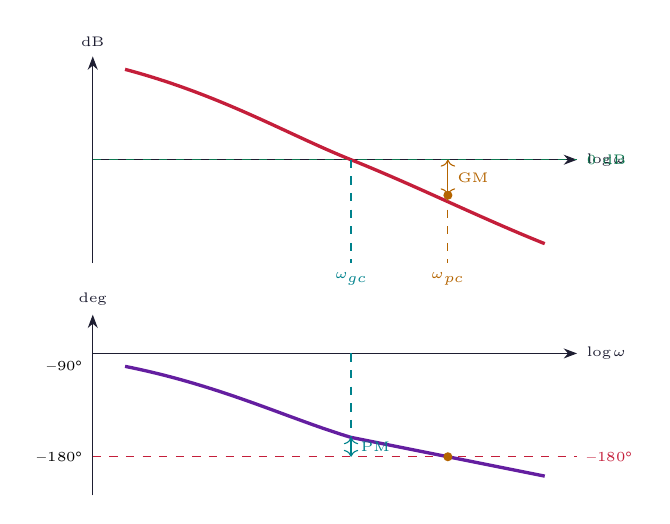
\begin{tikzpicture}[scale=0.82]
  % ── Magnitude plot ──
  \draw[axis] (0,1.8) -- (7.5,1.8) node[right,font=\tiny] {$\log\omega$};
  \draw[axis] (0,0.2) -- (0,3.4) node[above,font=\tiny] {dB};
  \draw[dashed,color=mygreen,thin] (0,1.8) -- (7.5,1.8) node[right,font=\tiny,color=mygreen] {0 dB};
  % Magnitude curve
  \draw[color=myred,line width=1.2pt]
    (0.5,3.2) .. controls (2,2.8) and (3,2.2) .. (4,1.8)
    .. controls (5,1.4) and (6,0.9) .. (7,0.5);
  % wgc marker
  \draw[dashed,color=myteal,thin] (4,1.8) -- (4,0.2) node[below,font=\tiny,color=myteal] {$\omega_{gc}$};
  % wpc marker
  \draw[dashed,color=myamber,thin] (5.5,1.8) -- (5.5,0.2) node[below,font=\tiny,color=myamber] {$\omega_{pc}$};
  % GM arrow
  \draw[<->,color=myamber,thin] (5.5,1.8) -- (5.5,1.25);
  \node[right,font=\tiny,color=myamber] at (5.5,1.52) {GM};
  \fill[myamber] (5.5,1.25) circle (2pt);
  % ── Phase plot ──
  \draw[axis] (0,-1.2) -- (7.5,-1.2) node[right,font=\tiny] {$\log\omega$};
  \draw[axis] (0,-3.4) -- (0,-0.6) node[above,font=\tiny] {deg};
  \draw[dashed,color=myred,thin] (0,-2.8) -- (7.5,-2.8) node[right,font=\tiny,color=myred] {$-180°$};
  % Phase curve
  \draw[color=mypurple,line width=1.2pt]
    (0.5,-1.4) .. controls (2,-1.7) and (3,-2.2) .. (4,-2.5)
    .. controls (5,-2.7) and (5.5,-2.8) .. (7,-3.1);
  % PM arrow at wgc
  \draw[<->,color=myteal,thin] (4,-2.5) -- (4,-2.8);
  \node[right,font=\tiny,color=myteal] at (4,-2.65) {PM};
  \draw[dashed,color=myteal,thin] (4,-1.2) -- (4,-2.5);
  % -180 at wpc
  \fill[myamber] (5.5,-2.8) circle (2pt);
  \node[left,font=\tiny] at (0,-1.4) {$-90°$};
  \node[left,font=\tiny] at (0,-2.8) {$-180°$};
\end{tikzpicture}
\end{tcolorbox}

\begin{tabularx}{\linewidth}{|B{3.2cm}|>{\centering\arraybackslash}X|>{\centering\arraybackslash}X|}
\hline
\multicolumn{1}{|>{\centering\arraybackslash}p{3.2cm}|}{\textbf{Margin}} &
\textbf{\color{myamber}Definition} & \textbf{\color{mygreen}Measurement Point} \\
\hline
Gain Margin (GM) & $1/|G(j\omega_{pc})|$ & At phase crossover freq $\omega_{pc}$ ($\angle = -180°$) \\
\hline
Phase Margin (PM) & $180° + \angle G(j\omega_{gc})$ & At gain crossover freq $\omega_{gc}$ ($|G|=1$) \\
\hline
Stable condition & $GM > 1$ ($>0$ dB) & $PM > 0°$ \\
\hline
Good design & $GM \geq 6$ dB & $PM = 30°$--$60°$ \\
\hline
\end{tabularx}

\begin{tcolorbox}[exambox, title={Exam Tips --- GM and PM}]
\begin{itemize}[leftmargin=*, itemsep=3pt, topsep=0pt]
  \item \textbf{GM} is read from the magnitude plot at $\omega_{pc}$; \textbf{PM} is read from the phase plot at $\omega_{gc}$.
  \item If the magnitude curve \textit{never} crosses 0 dB, $\omega_{gc}$ does not exist --- system is always stable for that gain.
  \item If the phase curve \textit{never} reaches $-180°$, $\omega_{pc}$ does not exist --- $GM = \infty$.
  \item \textbf{Higher PM} $\Rightarrow$ less overshoot, more damping. $PM \approx 100\zeta$ for $\zeta < 0.7$.
  \item \textbf{Conditionally stable systems} can have $GM > 0$ dB but become unstable if gain is \textit{reduced}.
\end{itemize}
\end{tcolorbox}

%═══════════════════════════════════════════════════════════════════════════════
\section{Nyquist Plot}
%═══════════════════════════════════════════════════════════════════════════════

\begin{tcolorbox}[defbox]
\textbf{Nyquist Plot:} The polar plot of $G(j\omega)H(j\omega)$ for $\omega$ varying from $-\infty$ to $+\infty$ (i.e., the complete Nyquist contour). It is the mirror image of the polar plot about the real axis for negative frequencies. Used to apply the \textbf{Nyquist Stability Criterion}.
\end{tcolorbox}

\subsection{Nyquist Contour}

The \textbf{Nyquist contour} $\Gamma_s$ in the $s$-plane encloses the entire right half-plane (RHP):
\begin{itemize}[leftmargin=*, itemsep=2pt]
  \item Segment 1: $s = j\omega$, $\omega: 0^+ \to +\infty$ (positive imaginary axis)
  \item Segment 2: $s = Re^{j\theta}$, $R\to\infty$, $\theta: +90° \to -90°$ (large semicircle)
  \item Segment 3: $s = j\omega$, $\omega: -\infty \to 0^-$ (negative imaginary axis)
  \item \textbf{Indentation:} Small semicircle of radius $\varepsilon\to 0$ around any poles on the imaginary axis.
\end{itemize}

\begin{tcolorbox}[tikzbox, title={Nyquist Contour in $s$-plane and Corresponding $G(j\omega)H(j\omega)$ Plot}]
\centering
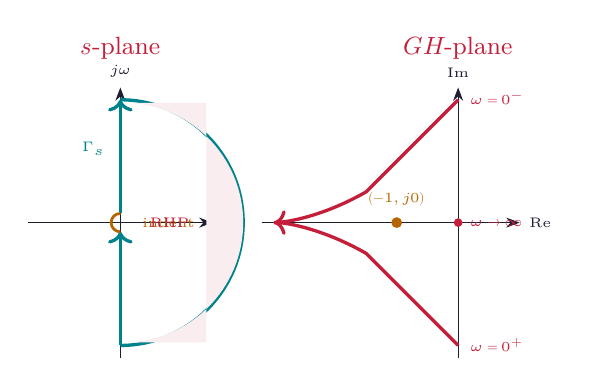
\begin{tikzpicture}[scale=0.78]
  % s-plane
  \begin{scope}[xshift=0cm]
    \draw[axis] (-1.5,0) -- (1.5,0) node[right,font=\tiny] {$\sigma$};
    \draw[axis] (0,-2.2) -- (0,2.2) node[above,font=\tiny] {$j\omega$};
    \node[above,font=\small,color=myred] at (0,2.5) {$s$-plane};
    % Nyquist contour
    \draw[color=myteal, line width=1.2pt, ->] (0,0.15) -- (0,2.0);
    \draw[color=myteal, line width=1.2pt] (0,2.0) arc(90:-90:2.0);
    \draw[color=myteal, line width=1.2pt, ->] (0,-2.0) -- (0,-0.15);
    % Indentation at origin
    \draw[color=myamber, line width=1.0pt] (0,0.15) arc(90:270:0.15);
    \node[left,font=\tiny,color=myteal] at (-0.1,1.2) {$\Gamma_s$};
    \node[right,font=\tiny,color=myamber] at (0.2,0) {indent};
    % RHP shading hint
    \fill[myred!8] (0.05,-1.95) arc(-90:90:1.95) -- (0.05,1.95) -- (1.4,1.95) -- (1.4,-1.95) -- cycle;
    \node[font=\tiny,color=myred] at (0.8,0) {RHP};
  \end{scope}
  % GH-plane
  \begin{scope}[xshift=5.5cm]
    \draw[axis] (-3.2,0) -- (1.0,0) node[right,font=\tiny] {Re};
    \draw[axis] (0,-2.2) -- (0,2.2) node[above,font=\tiny] {Im};
    \node[above,font=\small,color=myred] at (0,2.5) {$GH$-plane};
    % Nyquist plot (Type 1, 2nd order)
    \draw[color=myred, line width=1.2pt, ->]
      (0,-2.0) .. controls (-0.4,-1.6) and (-1.0,-1.0) .. (-1.5,-0.5)
      .. controls (-2.2,-0.1) and (-2.8,0) .. (-3.0,0);
    \draw[color=myred, line width=1.2pt]
      (0,2.0) .. controls (-0.4,1.6) and (-1.0,1.0) .. (-1.5,0.5)
      .. controls (-2.2,0.1) and (-2.8,0) .. (-3.0,0);
    % Large semicircle maps to origin
    \fill[myred] (0,0) circle (2pt);
    \node[right,font=\tiny,color=myred] at (0.05,0) {$\omega\to\infty$};
    % -1,0 point
    \fill[myamber] (-1,0) circle (2.5pt);
    \node[above,font=\tiny,color=myamber] at (-1,0.12) {$(-1,j0)$};
    % Labels
    \node[right,font=\tiny,color=myred] at (0.05,-2.0) {$\omega=0^+$};
    \node[right,font=\tiny,color=myred] at (0.05,2.0) {$\omega=0^-$};
  \end{scope}
\end{tikzpicture}
\end{tcolorbox}

%═══════════════════════════════════════════════════════════════════════════════
\section{Nyquist Stability Criterion}
%═══════════════════════════════════════════════════════════════════════════════

\begin{tcolorbox}[masonbox]
\textbf{Nyquist Stability Criterion:} Based on the \textbf{Principle of the Argument} (Cauchy's theorem). For a closed-loop system with open-loop transfer function $G(s)H(s)$:
$$N = Z - P$$
where:
\begin{itemize}[leftmargin=*, itemsep=2pt, topsep=2pt]
  \item $N$ = number of \textbf{clockwise encirclements} of the $(-1, j0)$ point by the Nyquist plot of $G(j\omega)H(j\omega)$.
  \item $Z$ = number of \textbf{closed-loop poles} in the RHP (zeros of $1+GH$).
  \item $P$ = number of \textbf{open-loop poles} of $G(s)H(s)$ in the RHP.
\end{itemize}
\textbf{For stability:} $Z = 0$, therefore $N = -P$ (i.e., $P$ \textit{counter-clockwise} encirclements if $P \neq 0$; no encirclements if $P = 0$).
\end{tcolorbox}

\subsection{Applying the Nyquist Criterion --- Step by Step}

\begin{enumerate}[label=\textbf{Step \arabic*:}, leftmargin=2.5cm, itemsep=4pt]
  \item Determine $P$ = number of open-loop poles of $G(s)H(s)$ in the RHP.
  \item Sketch the Nyquist plot of $G(j\omega)H(j\omega)$ for $\omega: 0^+ \to +\infty$.
  \item Mirror the plot about the real axis for $\omega: -\infty \to 0^-$.
  \item Handle poles on the $j\omega$-axis by indenting the contour (small semicircle of radius $\varepsilon\to0$).
  \item Count $N$ = net clockwise encirclements of $(-1, j0)$.
  \item Compute $Z = N + P$. If $Z = 0$: \textbf{stable}. If $Z > 0$: \textbf{unstable} ($Z$ RHP poles).
\end{enumerate}

\begin{tcolorbox}[examplebox, title={Example: $G(s)H(s) = K/[s(s+1)(s+2)]$, find stability range}]
\textbf{Open-loop poles:} $s=0$ (on $j\omega$-axis), $s=-1$, $s=-2$ (all in LHP). So $P=0$.

\textbf{Nyquist plot} crosses the negative real axis at $\omega_{pc}$ where $\angle G(j\omega)H(j\omega) = -180°$.

At $\omega_{pc}$: $\angle = -90° - \tan^{-1}(\omega) - \tan^{-1}(\omega/2) = -180°$
$\Rightarrow \tan^{-1}(\omega) + \tan^{-1}(\omega/2) = 90°$
$\Rightarrow \omega_{pc} = \sqrt{2}$ rad/s.

$|G(j\sqrt{2})H(j\sqrt{2})| = \dfrac{K}{\sqrt{2}\cdot\sqrt{3}\cdot\sqrt{4}} = \dfrac{K}{2\sqrt{6}}$

\textbf{For stability:} $N=0$ requires the plot does not encircle $(-1,j0)$:
$$\frac{K}{2\sqrt{6}} < 1 \;\Rightarrow\; K < 2\sqrt{6} \approx 4.9$$
\textbf{Gain Margin:} $GM = 2\sqrt{6}/K$. For $K=1$: $GM = 2\sqrt{6} \approx 4.9$ (13.8 dB).
\end{tcolorbox}

\subsection{Simplified Nyquist Criterion (Minimum Phase Systems)}

\begin{tcolorbox}[formulabox, title={For Minimum Phase Systems ($P=0$)}]
A minimum phase system (no open-loop RHP poles or zeros) is \textbf{closed-loop stable} if and only if the Nyquist plot of $G(j\omega)H(j\omega)$ does \textbf{not encircle} the $(-1, j0)$ point.\\[4pt]
Equivalently (from Bode plot): \textbf{stable} if $|G(j\omega_{pc})H(j\omega_{pc})| < 1$, i.e., $GM > 0$ dB \textbf{AND} $PM > 0°$.
\end{tcolorbox}

\begin{tcolorbox}[exambox, title={Exam Tips --- Nyquist Criterion}]
\begin{itemize}[leftmargin=*, itemsep=3pt, topsep=0pt]
  \item \textbf{$N = Z - P$} --- memorise this. $Z=0$ for stability.
  \item For \textbf{minimum phase} systems ($P=0$): stable iff no encirclement of $(-1,j0)$.
  \item \textbf{Clockwise} encirclement = positive $N$; \textbf{counter-clockwise} = negative $N$.
  \item Poles on $j\omega$-axis (e.g., integrators): indent contour to the right; the large semicircle maps to origin.
  \item The Nyquist plot is the \textbf{mirror image} of the polar plot about the real axis.
  \item \textbf{$(-1,j0)$ point} is the critical point --- corresponds to $|GH|=1$ and $\angle GH = -180°$.
\end{itemize}
\end{tcolorbox}

%═══════════════════════════════════════════════════════════════════════════════
\section{Performance Specifications in Frequency Domain}
%═══════════════════════════════════════════════════════════════════════════════

\begin{tcolorbox}[defbox]
\textbf{Frequency Domain Specifications} describe the closed-loop system's behaviour in terms of its frequency response $T(j\omega) = C(j\omega)/R(j\omega)$. They are directly related to time-domain performance.
\end{tcolorbox}

\subsection{Closed-Loop Frequency Response Specifications}

\begin{tabularx}{\linewidth}{|B{3.2cm}|>{\centering\arraybackslash}p{2.0cm}|X|}
\hline
\multicolumn{1}{|>{\centering\arraybackslash}p{3.2cm}|}{\textbf{\color{myteal}Specification}} &
\multicolumn{1}{>{\centering\arraybackslash}p{2.0cm}|}{\textbf{\color{myteal}Symbol}} &
\multicolumn{1}{>{\centering\arraybackslash}X|}{\textbf{\color{myteal}Definition}} \\
\hline
Resonant Peak & $M_r$ & Maximum value of $|T(j\omega)|$. Indicates relative stability; high $M_r$ means low damping. \\
\hline
Resonant Frequency & $\omega_r$ & Frequency at which $|T(j\omega)|$ is maximum. \\
\hline
Bandwidth & $\omega_{BW}$ & Frequency at which $|T(j\omega)|$ drops to $1/\sqrt{2}$ ($-3$ dB) of its DC value. Indicates speed of response. \\
\hline
Cutoff Rate & --- & Rate at which $|T(j\omega)|$ decreases beyond $\omega_{BW}$; indicates noise rejection. \\
\hline
\end{tabularx}

\subsection{Formulas for Second-Order System}

\begin{tcolorbox}[formulabox, title={Closed-Loop Frequency Response --- 2nd Order}]
For $T(s) = \omega_n^2/(s^2+2\zeta\omega_n s+\omega_n^2)$:
$$|T(j\omega)| = \frac{1}{\sqrt{(1-u^2)^2 + (2\zeta u)^2}}, \quad u = \omega/\omega_n$$
\textbf{Resonant frequency:} $\omega_r = \omega_n\sqrt{1-2\zeta^2}$ \quad (exists only for $\zeta < 1/\sqrt{2} \approx 0.707$)\\[4pt]
\textbf{Resonant peak:} $M_r = \dfrac{1}{2\zeta\sqrt{1-\zeta^2}}$ \quad (for $\zeta < 0.707$)\\[4pt]
\textbf{Bandwidth:} $\omega_{BW} = \omega_n\sqrt{(1-2\zeta^2)+\sqrt{4\zeta^4-4\zeta^2+2}}$
\end{tcolorbox}

\subsection{Relation Between Frequency and Time Domain Specs}

\begin{tabularx}{\linewidth}{|B{3.4cm}|>{\centering\arraybackslash}X|>{\centering\arraybackslash}X|}
\hline
\multicolumn{1}{|>{\centering\arraybackslash}p{3.4cm}|}{\textbf{Freq. Domain}} &
\textbf{\color{myamber}Relation} & \textbf{\color{mygreen}Time Domain Equivalent} \\
\hline
High $\omega_{BW}$ & $\omega_{BW} \propto \omega_n$ & Faster rise time, faster response \\
\hline
High $M_r$ & $M_r \uparrow$ as $\zeta \downarrow$ & High overshoot $M_p$ \\
\hline
$M_r = 1$ & $\zeta \geq 0.707$ & No overshoot (overdamped/critically) \\
\hline
Phase Margin & $PM \approx 100\zeta$ (for $\zeta < 0.7$) & Damping ratio $\zeta$ \\
\hline
Gain Margin & Larger GM & More stable, less sensitive to gain \\
\hline
$\omega_{gc}$ & $\omega_{gc} \approx \omega_{BW}$ & Bandwidth approximation \\
\hline
\end{tabularx}

\begin{tcolorbox}[tikzbox, title={Closed-Loop Frequency Response (Resonance Peak)}]
\centering
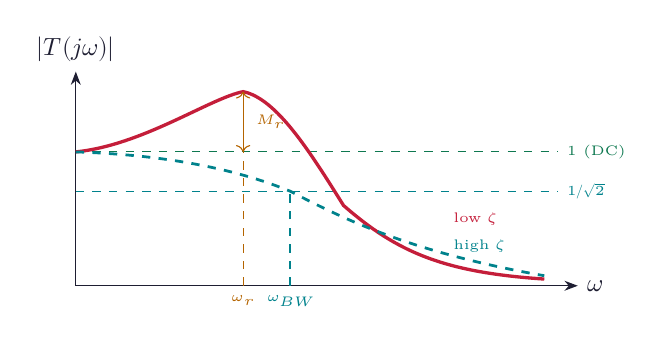
\begin{tikzpicture}[scale=0.85]
  \draw[axis] (0,0) -- (7.5,0) node[right,font=\small] {$\omega$};
  \draw[axis] (0,0) -- (0,3.2) node[above,font=\small] {$|T(j\omega)|$};
  % DC value = 1
  \draw[dashed,color=mygreen,thin] (0,2) -- (7.2,2) node[right,font=\tiny,color=mygreen] {$1$ (DC)};
  % -3dB line
  \draw[dashed,color=myteal,thin] (0,1.414) -- (7.2,1.414) node[right,font=\tiny,color=myteal] {$1/\sqrt{2}$};
  % Low damping curve (zeta=0.3)
  \draw[color=myred,line width=1.2pt]
    (0,2) .. controls (1,2.1) and (2,2.8) .. (2.5,2.9)
    .. controls (3,2.8) and (3.5,2.0) .. (4,1.2)
    .. controls (4.8,0.5) and (5.5,0.2) .. (7,0.1);
  % High damping curve (zeta=0.7)
  \draw[color=myteal,line width=1.0pt,dashed]
    (0,2) .. controls (1.5,1.95) and (2.5,1.7) .. (3.2,1.414)
    .. controls (4,1.0) and (5,0.5) .. (7,0.15);
  % Mr annotation
  \draw[<->,color=myamber,thin] (2.5,2) -- (2.5,2.9);
  \node[right,font=\tiny,color=myamber] at (2.55,2.45) {$M_r$};
  \draw[dashed,color=myamber,thin] (2.5,0) node[below,font=\tiny,color=myamber] {$\omega_r$} -- (2.5,2.9);
  % BW annotation
  \draw[dashed,color=myteal,thin] (3.2,0) node[below,font=\tiny,color=myteal] {$\omega_{BW}$} -- (3.2,1.414);
  % Legend
  \node[right,font=\tiny,color=myred] at (5.5,1.0) {low $\zeta$};
  \node[right,font=\tiny,color=myteal] at (5.5,0.6) {high $\zeta$};
\end{tikzpicture}
\end{tcolorbox}

\begin{tcolorbox}[exambox, title={Exam Tips --- Frequency Domain Specs}]
\begin{itemize}[leftmargin=*, itemsep=3pt, topsep=0pt]
  \item \textbf{$M_r > 1.3$} (about 2.3 dB) indicates poor relative stability (excessive overshoot).
  \item \textbf{$\omega_r < \omega_n$} always (resonant frequency is less than natural frequency).
  \item \textbf{$\omega_{BW} > \omega_n$} always (bandwidth exceeds natural frequency).
  \item \textbf{$PM \approx 100\zeta$} for $\zeta < 0.7$ --- very useful approximation in design.
  \item \textbf{Bandwidth} determines speed: wider BW = faster response but more noise.
  \item For $\zeta \geq 0.707$: $M_r = 1$ (no resonance peak); response is monotonically decreasing.
\end{itemize}
\end{tcolorbox}

%═══════════════════════════════════════════════════════════════════════════════
% QUICK REVISION --- MODULE 4
%═══════════════════════════════════════════════════════════════════════════════
\newpage
\begin{center}
  {\large\bfseries\color{myred} Quick Revision --- Module 4}\\[3pt]
  {\small\color{mydark} Frequency Response Analysis $|$ EC601}
\end{center}
\noindent{\color{myred}\rule{\linewidth}{1.2pt}}
\vspace{4pt}

\begin{tcolorbox}[formulabox, title={\textbf{Key Formulas at a Glance}}]
\begin{tabularx}{\linewidth}{B{5.2cm} X}
Frequency response          & $G(j\omega) = G(s)|_{s=j\omega}$ \\[2pt]
Gain Margin                 & $GM = 1/|G(j\omega_{pc})H(j\omega_{pc})|$ \\[2pt]
GM in dB                    & $GM_{dB} = -20\log|G(j\omega_{pc})|$ \\[2pt]
Phase Margin                & $PM = 180° + \angle G(j\omega_{gc})H(j\omega_{gc})$ \\[2pt]
Phase crossover freq        & $\omega_{pc}$: where $\angle GH = -180°$ \\[2pt]
Gain crossover freq         & $\omega_{gc}$: where $|GH| = 1$ (0 dB) \\[2pt]
Nyquist criterion           & $N = Z - P$; stable if $Z=0$ \\[2pt]
Resonant peak (2nd order)   & $M_r = 1/(2\zeta\sqrt{1-\zeta^2})$, $\zeta < 0.707$ \\[2pt]
Resonant frequency          & $\omega_r = \omega_n\sqrt{1-2\zeta^2}$ \\[2pt]
Bandwidth (2nd order)       & $\omega_{BW} = \omega_n\sqrt{(1-2\zeta^2)+\sqrt{4\zeta^4-4\zeta^2+2}}$ \\[2pt]
PM--damping relation        & $PM \approx 100\zeta$ (for $\zeta < 0.7$) \\[2pt]
Bode: simple pole slope     & $-20$ dB/dec above corner freq $\omega_c = 1/T$ \\[2pt]
Bode: double pole slope     & $-40$ dB/dec above $\omega_n$ \\[2pt]
Bode: phase at corner       & $-45°$ at $\omega_c$ for simple pole
\end{tabularx}
\end{tcolorbox}

\vspace{5pt}

\begin{tcolorbox}[defbox, title={\textbf{One-Line Definitions}}]
\begin{itemize}[leftmargin=*, itemsep=3pt, topsep=0pt]
  \item \textbf{Frequency Response:} System's steady-state response to sinusoidal input; $G(j\omega)$.
  \item \textbf{Polar Plot:} Locus of $G(j\omega)$ in complex plane as $\omega: 0\to\infty$.
  \item \textbf{Bode Plot:} Semi-log plots of magnitude (dB) and phase (deg) vs $\log\omega$.
  \item \textbf{Corner Frequency:} $\omega_c = 1/T$; slope changes by $\pm20$ dB/dec here.
  \item \textbf{Gain Crossover Freq $\omega_{gc}$:} Where $|GH|=1$ (0 dB); PM is measured here.
  \item \textbf{Phase Crossover Freq $\omega_{pc}$:} Where $\angle GH = -180°$; GM is measured here.
  \item \textbf{Gain Margin:} Factor by which gain can increase before instability; $GM > 0$ dB for stability.
  \item \textbf{Phase Margin:} Additional phase lag before instability; $PM > 0°$ for stability.
  \item \textbf{Nyquist Plot:} Polar plot of $GH(j\omega)$ for $\omega: -\infty\to+\infty$.
  \item \textbf{Nyquist Criterion:} $N=Z-P$; stable if $Z=0$ (no RHP closed-loop poles).
  \item \textbf{Resonant Peak $M_r$:} Maximum of $|T(j\omega)|$; indicates damping ($M_r\uparrow$ as $\zeta\downarrow$).
  \item \textbf{Bandwidth $\omega_{BW}$:} Freq where $|T|$ drops to $-3$ dB; indicates response speed.
  \item \textbf{Minimum Phase System:} No RHP poles or zeros; $P=0$; stable iff no encirclement of $(-1,j0)$.
\end{itemize}
\end{tcolorbox}

\vspace{5pt}

\begin{tcolorbox}[exambox, title={\textbf{Frequently Asked / Viva Questions}}]
\begin{enumerate}[leftmargin=*, topsep=0pt, label=\textbf{Q\arabic*.}, itemsep=8pt]
  \item \Q{What is the frequency response of a system?} The steady-state output-to-input ratio for sinusoidal inputs; obtained by substituting $s=j\omega$ in $G(s)$.
  \item \Q{What is the gain crossover frequency?} The frequency $\omega_{gc}$ where $|G(j\omega)H(j\omega)|=1$ (0 dB). Phase margin is measured here.
  \item \Q{What is the phase crossover frequency?} The frequency $\omega_{pc}$ where $\angle G(j\omega)H(j\omega)=-180°$. Gain margin is measured here.
  \item \Q{Define Gain Margin.} $GM = 1/|GH(j\omega_{pc})|$. It is the factor by which gain can be increased before instability. Stable if $GM > 1$ (0 dB).
  \item \Q{Define Phase Margin.} $PM = 180° + \angle GH(j\omega_{gc})$. Additional phase lag before instability. Stable if $PM > 0°$.
  \item \Q{State the Nyquist stability criterion.} $N = Z - P$. For stability $Z=0$, so $N=-P$. For minimum phase ($P=0$): no encirclement of $(-1,j0)$.
  \item \Q{What is $N$, $Z$, $P$ in Nyquist criterion?} $N$ = clockwise encirclements of $(-1,j0)$; $Z$ = RHP closed-loop poles; $P$ = RHP open-loop poles.
  \item \Q{What is the slope of Bode magnitude plot for a simple pole?} $-20$ dB/decade above the corner frequency $\omega_c = 1/T$.
  \item \Q{What is the resonant peak $M_r$?} Maximum value of closed-loop frequency response; $M_r = 1/(2\zeta\sqrt{1-\zeta^2})$ for 2nd order. Exists only for $\zeta < 0.707$.
  \item \Q{What is bandwidth?} Frequency at which $|T(j\omega)|$ drops to $1/\sqrt{2}$ ($-3$ dB) of DC value. Wider BW = faster response.
  \item \Q{Relation between PM and damping ratio?} $PM \approx 100\zeta$ for $\zeta < 0.7$. So $PM = 45°$ corresponds to $\zeta \approx 0.45$.
  \item \Q{What is a minimum phase system?} A system with no RHP poles or zeros and no time delay. Its Bode magnitude uniquely determines the phase.
\end{enumerate}
\end{tcolorbox}

\vspace{5pt}

\begin{tcolorbox}[tikzbox, title={\textbf{Stability Summary}}]
\begin{tabularx}{\linewidth}{|>{\centering\arraybackslash}X|>{\centering\arraybackslash}X|>{\centering\arraybackslash}X|}
\hline
\textbf{\color{myteal}Condition} & \textbf{\color{mygreen}Stable} & \textbf{\color{myred}Unstable} \\
\hline
Gain Margin & $GM > 1$ ($> 0$ dB) & $GM < 1$ ($< 0$ dB) \\
\hline
Phase Margin & $PM > 0°$ & $PM < 0°$ \\
\hline
Nyquist ($P=0$) & No encirclement of $(-1,j0)$ & Encircles $(-1,j0)$ \\
\hline
Nyquist (general) & $Z = N + P = 0$ & $Z = N + P > 0$ \\
\hline
Bode (min. phase) & $\omega_{gc} < \omega_{pc}$ & $\omega_{gc} > \omega_{pc}$ \\
\hline
\end{tabularx}
\end{tcolorbox}


% -- Module 5 -----------------------------------------------------------------
\modulestart{5}{State Variable Analysis --- Introduction}

\section{State Variable Analysis --- Introduction}
%═══════════════════════════════════════════════════════════════════════════════

Classical control (transfer function approach) describes a system only in terms of its input-output relationship and is limited to LTI, SISO systems. \textbf{State variable analysis} (modern control) provides a complete internal description of the system, handles MIMO systems, time-varying systems, and nonlinear systems, and is directly suited for computer-based design.

\begin{tcolorbox}[defbox]
\textbf{State:} The state of a system at time $t_0$ is the minimum set of variables (state variables) that, together with the input for $t \geq t_0$, completely determines the future behaviour of the system.\\[4pt]
\textbf{State Variable:} Each member of the minimum set of variables that completely describes the state of the system. For an $n$-th order system, there are exactly $n$ state variables.\\[4pt]
\textbf{State Vector:} The column vector $\mathbf{x}(t) = [x_1(t),\, x_2(t),\, \ldots,\, x_n(t)]^T$ formed by all $n$ state variables.\\[4pt]
\textbf{State Space:} The $n$-dimensional space whose axes are the state variables $x_1, x_2, \ldots, x_n$. Each point in state space represents a unique state of the system.
\end{tcolorbox}

\subsection{Why State Variables?}

\begin{tabularx}{\linewidth}{|B{3.4cm}|>{\centering\arraybackslash}X|>{\centering\arraybackslash}X|}
\hline
\multicolumn{1}{|>{\centering\arraybackslash}p{3.4cm}|}{\textbf{Aspect}} &
\textbf{\color{myamber}Transfer Function} & \textbf{\color{mygreen}State Space} \\
\hline
System type & SISO, LTI only & MIMO, nonlinear, time-varying \\
\hline
Internal info & No (black box) & Yes (complete internal description) \\
\hline
Initial conditions & Difficult to handle & Naturally included \\
\hline
Computer design & Indirect & Direct (matrix methods) \\
\hline
Stability analysis & Characteristic equation & Eigenvalues of $\mathbf{A}$ matrix \\
\hline
Design methods & Root locus, Bode & Pole placement, optimal control \\
\hline
\end{tabularx}

%═══════════════════════════════════════════════════════════════════════════════
\section{State Space Representation}
%═══════════════════════════════════════════════════════════════════════════════

\begin{tcolorbox}[formulabox, title={Standard State Space Form}]
\textbf{State equation:}
$$\dot{\mathbf{x}}(t) = \mathbf{A}\,\mathbf{x}(t) + \mathbf{B}\,\mathbf{u}(t)$$
\textbf{Output equation:}
$$\mathbf{y}(t) = \mathbf{C}\,\mathbf{x}(t) + \mathbf{D}\,\mathbf{u}(t)$$
where:
\begin{itemize}[leftmargin=*, itemsep=2pt, topsep=2pt]
  \item $\mathbf{x}(t) \in \mathbb{R}^n$ --- state vector ($n$ state variables)
  \item $\mathbf{u}(t) \in \mathbb{R}^r$ --- input vector ($r$ inputs)
  \item $\mathbf{y}(t) \in \mathbb{R}^m$ --- output vector ($m$ outputs)
  \item $\mathbf{A}$ ($n\times n$) --- system/plant matrix (dynamics)
  \item $\mathbf{B}$ ($n\times r$) --- input matrix
  \item $\mathbf{C}$ ($m\times n$) --- output matrix
  \item $\mathbf{D}$ ($m\times r$) --- direct transmission (feedthrough) matrix
\end{itemize}
\end{tcolorbox}

\begin{tcolorbox}[tikzbox, title={State Space Block Diagram}]
\centering
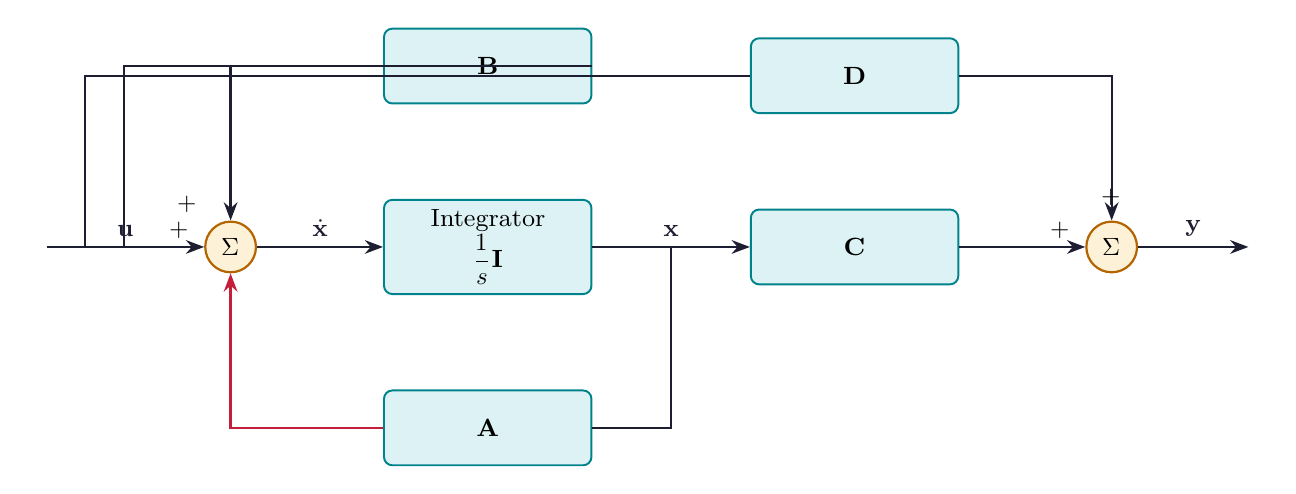
\begin{tikzpicture}[node distance=0.6cm and 1.4cm]
  % Main forward path nodes
  \node[sumjunc] (sum) {$\Sigma$};
  \node[block, right=1.6cm of sum] (int) {Integrator\\$\dfrac{1}{s}\mathbf{I}$};
  \node[block, right=2.0cm of int] (C) {$\mathbf{C}$};
  \node[sumjunc, right=1.6cm of C] (osum) {$\Sigma$};
  % Input / output terminals
  \node[left=2.0cm of sum] (u) {};
  \node[right=1.4cm of osum] (y) {};
  % A feedback block (below integrator)
  \node[block, below=1.2cm of int] (A) {$\mathbf{A}$};
  % B block (above integrator, between sum and int)
  \node[block, above=1.2cm of int] (B) {$\mathbf{B}$};
  % D block (above C, feedthrough)
  \node[block, above=1.2cm of C] (D) {$\mathbf{D}$};

  % ── Main signal path ──────────────────────────────────────────────────────
  \draw[arrow] (u)   -- node[above]{\small $\mathbf{u}$} (sum);
  \draw[arrow] (sum) -- node[above]{\small $\dot{\mathbf{x}}$} (int);
  \draw[arrow] (int) -- node[above]{\small $\mathbf{x}$} (C);
  \draw[arrow] (C)   -- (osum);
  \draw[arrow] (osum)-- node[above]{\small $\mathbf{y}$} (y);

  % ── B path: tap from input wire → B block → sum (top) ────────────────────
  \coordinate (utap) at ($(u)!0.45!(sum)$);
  \draw[line]  (utap) |- (B.west);
  \draw[arrow] (B.east) -| (sum.north);

  % ── D path: tap from input wire → D block → output sum (top) ─────────────
  \coordinate (utap2) at ($(u)!0.25!(sum)$);
  \draw[line]  (utap2) |- (D.west);
  \draw[arrow] (D.east) -| (osum.north);

  % ── A feedback: tap from x wire → A block → sum (south) ──────────────────
  \coordinate (xtap) at ($(int.east)!0.5!(C.west)$);
  \draw[line]     (xtap) |- (A.east);
  \draw[redarrow] (A.west) -| (sum.south);

  % ── Sign labels ───────────────────────────────────────────────────────────
  \node[above left=2pt and 2pt of sum]{\small $+$};
  \node[left=2pt of sum, yshift=6pt]{\small $+$};
  \node[above=2pt of osum]{\small $+$};
  \node[left=2pt of osum, yshift=6pt]{\small $+$};
\end{tikzpicture}
\end{tcolorbox}

\subsection{Choosing State Variables}

For a physical system, state variables are typically the \textbf{energy storage variables}:
\begin{itemize}[leftmargin=*, itemsep=2pt]
  \item \textbf{Electrical circuits:} Capacitor voltages $v_C$ and inductor currents $i_L$
  \item \textbf{Mechanical systems:} Displacement $x$ and velocity $\dot{x}$
  \item \textbf{Thermal systems:} Temperatures at each node
\end{itemize}

For an $n$-th order ODE, the standard choice is the \textbf{phase variable form}: $x_1 = y,\; x_2 = \dot{y},\; \ldots,\; x_n = y^{(n-1)}$.

\subsection{Phase Variable Form --- Example}

\begin{tcolorbox}[examplebox, title={Example: 3rd Order System}]
\textbf{Given ODE:} $\dddot{y} + a_2\ddot{y} + a_1\dot{y} + a_0 y = b_0 u$

\textbf{State variables:} $x_1 = y,\quad x_2 = \dot{y},\quad x_3 = \ddot{y}$

\textbf{State equations:}
\begin{align*}
\dot{x}_1 &= x_2 \\
\dot{x}_2 &= x_3 \\
\dot{x}_3 &= -a_0 x_1 - a_1 x_2 - a_2 x_3 + b_0 u
\end{align*}

\textbf{Matrix form:}
$$\begin{bmatrix}\dot{x}_1\\\dot{x}_2\\\dot{x}_3\end{bmatrix}
= \underbrace{\begin{bmatrix}0&1&0\\0&0&1\\-a_0&-a_1&-a_2\end{bmatrix}}_{\mathbf{A}}
\begin{bmatrix}x_1\\x_2\\x_3\end{bmatrix}
+ \underbrace{\begin{bmatrix}0\\0\\b_0\end{bmatrix}}_{\mathbf{B}} u, \qquad
y = \underbrace{\begin{bmatrix}1&0&0\end{bmatrix}}_{\mathbf{C}}\mathbf{x}$$

The $\mathbf{A}$ matrix in this form is called the \textbf{companion matrix} or \textbf{phase variable canonical form}.
\end{tcolorbox}

%═══════════════════════════════════════════════════════════════════════════════
\section{State Transition Matrix (STM)}
%═══════════════════════════════════════════════════════════════════════════════

\begin{tcolorbox}[defbox]
\textbf{State Transition Matrix (STM)} $\boldsymbol{\Phi}(t)$: Also called the \textbf{matrix exponential} $e^{\mathbf{A}t}$. It describes how the state vector transitions from its initial value $\mathbf{x}(0)$ to $\mathbf{x}(t)$ in the absence of any input (homogeneous case):
$$\mathbf{x}(t) = \boldsymbol{\Phi}(t)\,\mathbf{x}(0) = e^{\mathbf{A}t}\,\mathbf{x}(0)$$
\end{tcolorbox}

\subsection{Definition and Computation}

\begin{tcolorbox}[formulabox, title={Matrix Exponential --- Definition}]
$$\boldsymbol{\Phi}(t) = e^{\mathbf{A}t} = \mathbf{I} + \mathbf{A}t + \frac{\mathbf{A}^2 t^2}{2!} + \frac{\mathbf{A}^3 t^3}{3!} + \cdots = \sum_{k=0}^{\infty}\frac{(\mathbf{A}t)^k}{k!}$$
\end{tcolorbox}

\textbf{Methods to compute $e^{\mathbf{A}t}$:}

\begin{enumerate}[label=\textbf{\arabic*.}, leftmargin=*, itemsep=4pt]
  \item \textbf{Infinite series} (above) --- impractical for large $n$.
  \item \textbf{Laplace transform method:} $\boldsymbol{\Phi}(t) = \mathcal{L}^{-1}\{(s\mathbf{I}-\mathbf{A})^{-1}\}$
  \item \textbf{Cayley-Hamilton theorem:} Express $e^{\mathbf{A}t}$ as a polynomial in $\mathbf{A}$ of degree $\leq n-1$.
  \item \textbf{Diagonalisation:} If $\mathbf{A} = \mathbf{P}\mathbf{\Lambda}\mathbf{P}^{-1}$, then $e^{\mathbf{A}t} = \mathbf{P}\,e^{\mathbf{\Lambda}t}\,\mathbf{P}^{-1}$.
\end{enumerate}

\begin{tcolorbox}[formulabox, title={Laplace Method (Most Exam-Relevant)}]
$$\boldsymbol{\Phi}(t) = e^{\mathbf{A}t} = \mathcal{L}^{-1}\left\{(s\mathbf{I} - \mathbf{A})^{-1}\right\}$$
\textbf{Steps:}
\begin{enumerate}[label=\arabic*., leftmargin=*, itemsep=2pt, topsep=2pt]
  \item Form $(s\mathbf{I} - \mathbf{A})$ by subtracting $\mathbf{A}$ from $s$ times the identity matrix.
  \item Compute the inverse: $(s\mathbf{I} - \mathbf{A})^{-1} = \dfrac{\text{adj}(s\mathbf{I}-\mathbf{A})}{\det(s\mathbf{I}-\mathbf{A})}$
  \item Take the inverse Laplace transform of each element.
\end{enumerate}
\end{tcolorbox}

\subsection{Properties of the STM}

\begin{tabularx}{\linewidth}{|>{\centering\arraybackslash}p{0.6cm}|B{4.0cm}|X|}
\hline
\multicolumn{1}{|>{\centering\arraybackslash}p{0.6cm}|}{\textbf{\color{myteal}\#}} &
\multicolumn{1}{>{\centering\arraybackslash}p{4.0cm}|}{\textbf{\color{myteal}Property}} &
\multicolumn{1}{>{\centering\arraybackslash}X|}{\textbf{\color{myteal}Expression}} \\
\hline
1 & Initial value & $\boldsymbol{\Phi}(0) = \mathbf{I}$ (identity matrix) \\
\hline
2 & Inverse & $\boldsymbol{\Phi}^{-1}(t) = \boldsymbol{\Phi}(-t) = e^{-\mathbf{A}t}$ \\
\hline
3 & Composition & $\boldsymbol{\Phi}(t_1+t_2) = \boldsymbol{\Phi}(t_1)\,\boldsymbol{\Phi}(t_2)$ \\
\hline
4 & Derivative & $\dot{\boldsymbol{\Phi}}(t) = \mathbf{A}\,\boldsymbol{\Phi}(t) = \boldsymbol{\Phi}(t)\,\mathbf{A}$ \\
\hline
5 & Transition & $\boldsymbol{\Phi}(t_2 - t_1) = \boldsymbol{\Phi}(t_2)\,\boldsymbol{\Phi}^{-1}(t_1)$ \\
\hline
6 & Determinant & $\det[\boldsymbol{\Phi}(t)] = e^{\text{tr}(\mathbf{A})\cdot t} \neq 0$ (always non-singular) \\
\hline
\end{tabularx}

\begin{tcolorbox}[examplebox, title={Example: Compute STM for $\mathbf{A} = \begin{bmatrix}0&1\\-2&-3\end{bmatrix}$}]
$(s\mathbf{I}-\mathbf{A}) = \begin{bmatrix}s&-1\\2&s+3\end{bmatrix}$

$\det(s\mathbf{I}-\mathbf{A}) = s(s+3)+2 = s^2+3s+2 = (s+1)(s+2)$

$(s\mathbf{I}-\mathbf{A})^{-1} = \dfrac{1}{(s+1)(s+2)}\begin{bmatrix}s+3&1\\-2&s\end{bmatrix}$

Using partial fractions and inverse Laplace:
$$\boldsymbol{\Phi}(t) = \begin{bmatrix}2e^{-t}-e^{-2t} & e^{-t}-e^{-2t}\\-2e^{-t}+2e^{-2t} & -e^{-t}+2e^{-2t}\end{bmatrix}$$
\end{tcolorbox}

%═══════════════════════════════════════════════════════════════════════════════
\section{Solution of State Equations}
%═══════════════════════════════════════════════════════════════════════════════

\subsection{Homogeneous State Equation (Zero Input)}

When $\mathbf{u}(t) = \mathbf{0}$, the state equation reduces to:
$$\dot{\mathbf{x}}(t) = \mathbf{A}\,\mathbf{x}(t)$$

\begin{tcolorbox}[formulabox, title={Solution --- Homogeneous (Zero Input)}]
$$\boxed{\mathbf{x}(t) = e^{\mathbf{A}t}\,\mathbf{x}(0) = \boldsymbol{\Phi}(t)\,\mathbf{x}(0)}$$
This is the \textbf{free response} or \textbf{zero-input response}. It depends only on the initial state $\mathbf{x}(0)$ and the system matrix $\mathbf{A}$.\\[4pt]
The output is: $\mathbf{y}(t) = \mathbf{C}\,\boldsymbol{\Phi}(t)\,\mathbf{x}(0)$
\end{tcolorbox}

\textbf{Derivation:} Assume $\mathbf{x}(t) = e^{\mathbf{A}t}\mathbf{c}$. Then $\dot{\mathbf{x}} = \mathbf{A}e^{\mathbf{A}t}\mathbf{c} = \mathbf{A}\mathbf{x}$ ✓. At $t=0$: $\mathbf{x}(0) = \mathbf{c}$. Hence $\mathbf{x}(t) = e^{\mathbf{A}t}\mathbf{x}(0)$.

\subsection{Non-Homogeneous State Equation (With Input)}

When $\mathbf{u}(t) \neq \mathbf{0}$:
$$\dot{\mathbf{x}}(t) = \mathbf{A}\,\mathbf{x}(t) + \mathbf{B}\,\mathbf{u}(t)$$

\begin{tcolorbox}[formulabox, title={Solution --- Non-Homogeneous (With Input)}]
$$\boxed{\mathbf{x}(t) = \underbrace{e^{\mathbf{A}t}\,\mathbf{x}(0)}_{\text{zero-input}} + \underbrace{\int_0^t e^{\mathbf{A}(t-\tau)}\,\mathbf{B}\,\mathbf{u}(\tau)\,d\tau}_{\text{zero-state (convolution)}}}$$
$$= \boldsymbol{\Phi}(t)\,\mathbf{x}(0) + \int_0^t \boldsymbol{\Phi}(t-\tau)\,\mathbf{B}\,\mathbf{u}(\tau)\,d\tau$$
\textbf{Output:}
$$\mathbf{y}(t) = \mathbf{C}\,\boldsymbol{\Phi}(t)\,\mathbf{x}(0) + \int_0^t \mathbf{C}\,\boldsymbol{\Phi}(t-\tau)\,\mathbf{B}\,\mathbf{u}(\tau)\,d\tau + \mathbf{D}\,\mathbf{u}(t)$$
\end{tcolorbox}

\textbf{Derivation (variation of parameters):} Multiply both sides of $\dot{\mathbf{x}} - \mathbf{A}\mathbf{x} = \mathbf{B}\mathbf{u}$ by the integrating factor $e^{-\mathbf{A}t}$:
$$\frac{d}{dt}\left[e^{-\mathbf{A}t}\mathbf{x}(t)\right] = e^{-\mathbf{A}t}\mathbf{B}\mathbf{u}(t)$$
Integrating from $0$ to $t$ and multiplying by $e^{\mathbf{A}t}$ gives the result above.

\subsection{Laplace Domain Solution}

Taking the Laplace transform of $\dot{\mathbf{x}} = \mathbf{A}\mathbf{x} + \mathbf{B}\mathbf{u}$:

\begin{tcolorbox}[formulabox, title={Laplace Domain Solution}]
$$s\mathbf{X}(s) - \mathbf{x}(0) = \mathbf{A}\mathbf{X}(s) + \mathbf{B}\mathbf{U}(s)$$
$$(s\mathbf{I} - \mathbf{A})\mathbf{X}(s) = \mathbf{x}(0) + \mathbf{B}\mathbf{U}(s)$$
$$\mathbf{X}(s) = (s\mathbf{I}-\mathbf{A})^{-1}\mathbf{x}(0) + (s\mathbf{I}-\mathbf{A})^{-1}\mathbf{B}\mathbf{U}(s)$$
$$\mathbf{Y}(s) = \mathbf{C}(s\mathbf{I}-\mathbf{A})^{-1}\mathbf{x}(0) + \left[\mathbf{C}(s\mathbf{I}-\mathbf{A})^{-1}\mathbf{B} + \mathbf{D}\right]\mathbf{U}(s)$$
\end{tcolorbox}

%═══════════════════════════════════════════════════════════════════════════════
\section{Transfer Function from State Space}
%═══════════════════════════════════════════════════════════════════════════════

\begin{tcolorbox}[defbox]
The \textbf{transfer function matrix} $\mathbf{G}(s)$ relates the output $\mathbf{Y}(s)$ to the input $\mathbf{U}(s)$ with zero initial conditions $[\mathbf{x}(0) = \mathbf{0}]$:
$$\mathbf{G}(s) = \frac{\mathbf{Y}(s)}{\mathbf{U}(s)}\bigg|_{\mathbf{x}(0)=\mathbf{0}}$$
\end{tcolorbox}

\begin{tcolorbox}[formulabox, title={Transfer Function from State Space (Zero I.C.)}]
Setting $\mathbf{x}(0) = \mathbf{0}$ in the Laplace solution:
$$\mathbf{Y}(s) = \left[\mathbf{C}(s\mathbf{I}-\mathbf{A})^{-1}\mathbf{B} + \mathbf{D}\right]\mathbf{U}(s)$$
$$\boxed{\mathbf{G}(s) = \mathbf{C}(s\mathbf{I}-\mathbf{A})^{-1}\mathbf{B} + \mathbf{D}}$$
For SISO systems ($\mathbf{D}=0$ typically): $G(s) = \mathbf{C}(s\mathbf{I}-\mathbf{A})^{-1}\mathbf{B}$\\[4pt]
The \textbf{characteristic polynomial} is $\det(s\mathbf{I}-\mathbf{A})$, whose roots are the \textbf{eigenvalues} of $\mathbf{A}$ = poles of the system.
\end{tcolorbox}

\begin{tcolorbox}[examplebox, title={Example: TF from State Space}]
\textbf{Given:} $\mathbf{A}=\begin{bmatrix}0&1\\-2&-3\end{bmatrix}$, $\mathbf{B}=\begin{bmatrix}0\\1\end{bmatrix}$, $\mathbf{C}=\begin{bmatrix}1&0\end{bmatrix}$, $D=0$

$(s\mathbf{I}-\mathbf{A}) = \begin{bmatrix}s&-1\\2&s+3\end{bmatrix}$, \quad $\det = s^2+3s+2$

$(s\mathbf{I}-\mathbf{A})^{-1} = \dfrac{1}{s^2+3s+2}\begin{bmatrix}s+3&1\\-2&s\end{bmatrix}$

$G(s) = \mathbf{C}(s\mathbf{I}-\mathbf{A})^{-1}\mathbf{B} = \dfrac{1}{s^2+3s+2}\begin{bmatrix}1&0\end{bmatrix}\begin{bmatrix}s+3&1\\-2&s\end{bmatrix}\begin{bmatrix}0\\1\end{bmatrix} = \dfrac{1}{s^2+3s+2}$
\end{tcolorbox}

\begin{tcolorbox}[exambox, title={Exam Tips --- State Space \& STM}]
\begin{itemize}[leftmargin=*, itemsep=3pt, topsep=0pt]
  \item \textbf{STM} $= e^{\mathbf{A}t} = \mathcal{L}^{-1}\{(s\mathbf{I}-\mathbf{A})^{-1}\}$ --- Laplace method is fastest in exams.
  \item \textbf{Homogeneous solution:} $\mathbf{x}(t) = e^{\mathbf{A}t}\mathbf{x}(0)$ --- zero input, only initial state.
  \item \textbf{Non-homogeneous solution:} zero-input + zero-state (convolution integral).
  \item \textbf{TF from SS:} $G(s) = \mathbf{C}(s\mathbf{I}-\mathbf{A})^{-1}\mathbf{B} + \mathbf{D}$ --- set $\mathbf{x}(0)=\mathbf{0}$.
  \item \textbf{Poles} of the system = eigenvalues of $\mathbf{A}$ = roots of $\det(s\mathbf{I}-\mathbf{A})=0$.
  \item \textbf{$\boldsymbol{\Phi}(0) = \mathbf{I}$} always --- a quick check to verify your STM computation.
\end{itemize}
\end{tcolorbox}

%═══════════════════════════════════════════════════════════════════════════════
\section{Controllability}
%═══════════════════════════════════════════════════════════════════════════════

\begin{tcolorbox}[defbox]
\textbf{Controllability:} A system is said to be \textbf{completely state controllable} if it is possible to transfer the system from \textit{any} initial state $\mathbf{x}(t_0)$ to \textit{any} desired final state $\mathbf{x}(t_f)$ in a finite time $t_f - t_0$ using an unconstrained control input $\mathbf{u}(t)$.\\[4pt]
In simple terms: \textit{Can the input reach and control every state variable?}
\end{tcolorbox}

\subsection{Kalman's Controllability Test}

\begin{tcolorbox}[formulabox, title={Controllability Matrix}]
The system $(\mathbf{A}, \mathbf{B})$ is \textbf{completely controllable} if and only if the \textbf{controllability matrix} $\mathbf{Q}_c$ has full rank $n$:
$$\mathbf{Q}_c = \begin{bmatrix}\mathbf{B} & \mathbf{A}\mathbf{B} & \mathbf{A}^2\mathbf{B} & \cdots & \mathbf{A}^{n-1}\mathbf{B}\end{bmatrix}$$
$$\text{rank}(\mathbf{Q}_c) = n \quad \Leftrightarrow \quad \det(\mathbf{Q}_c) \neq 0 \quad \Leftrightarrow \quad \text{System is controllable}$$
$\mathbf{Q}_c$ is an $n \times nr$ matrix (for SISO: $n \times n$ square matrix).
\end{tcolorbox}

\begin{tcolorbox}[examplebox, title={Example: Check Controllability}]
\textbf{Given:} $\mathbf{A}=\begin{bmatrix}0&1\\-2&-3\end{bmatrix}$, $\mathbf{B}=\begin{bmatrix}0\\1\end{bmatrix}$, $n=2$

$\mathbf{A}\mathbf{B} = \begin{bmatrix}0&1\\-2&-3\end{bmatrix}\begin{bmatrix}0\\1\end{bmatrix} = \begin{bmatrix}1\\-3\end{bmatrix}$

$\mathbf{Q}_c = \begin{bmatrix}\mathbf{B} & \mathbf{A}\mathbf{B}\end{bmatrix} = \begin{bmatrix}0&1\\1&-3\end{bmatrix}$

$\det(\mathbf{Q}_c) = (0)(-3) - (1)(1) = -1 \neq 0$

\textbf{Result:} $\text{rank}(\mathbf{Q}_c) = 2 = n$ $\Rightarrow$ System is \textbf{completely controllable}.
\end{tcolorbox}

\subsection{Physical Interpretation}

\begin{itemize}[leftmargin=*, itemsep=3pt]
  \item If a system is \textbf{not controllable}, some state variables are \textit{decoupled} from the input --- no matter what $\mathbf{u}(t)$ is applied, those states cannot be driven to a desired value.
  \item \textbf{Pole placement} (assigning closed-loop poles arbitrarily) is possible \textit{only if} the system is completely controllable.
  \item An uncontrollable mode corresponds to a pole of the system that cannot be moved by state feedback.
\end{itemize}

%═══════════════════════════════════════════════════════════════════════════════
\section{Observability}
%═══════════════════════════════════════════════════════════════════════════════

\begin{tcolorbox}[defbox]
\textbf{Observability:} A system is said to be \textbf{completely observable} if every state variable $x_i(t_0)$ can be determined from the output $\mathbf{y}(t)$ over a finite time interval $[t_0, t_f]$, given the input $\mathbf{u}(t)$.\\[4pt]
In simple terms: \textit{Can we reconstruct every state variable by observing the output?}
\end{tcolorbox}

\subsection{Kalman's Observability Test}

\begin{tcolorbox}[formulabox, title={Observability Matrix}]
The system $(\mathbf{A}, \mathbf{C})$ is \textbf{completely observable} if and only if the \textbf{observability matrix} $\mathbf{Q}_o$ has full rank $n$:
$$\mathbf{Q}_o = \begin{bmatrix}\mathbf{C}\\\mathbf{C}\mathbf{A}\\\mathbf{C}\mathbf{A}^2\\\vdots\\\mathbf{C}\mathbf{A}^{n-1}\end{bmatrix}$$
$$\text{rank}(\mathbf{Q}_o) = n \quad \Leftrightarrow \quad \det(\mathbf{Q}_o) \neq 0 \quad \Leftrightarrow \quad \text{System is observable}$$
$\mathbf{Q}_o$ is an $mn \times n$ matrix (for SISO: $n \times n$ square matrix).
\end{tcolorbox}

\begin{tcolorbox}[examplebox, title={Example: Check Observability}]
\textbf{Given:} $\mathbf{A}=\begin{bmatrix}0&1\\-2&-3\end{bmatrix}$, $\mathbf{C}=\begin{bmatrix}1&0\end{bmatrix}$, $n=2$

$\mathbf{C}\mathbf{A} = \begin{bmatrix}1&0\end{bmatrix}\begin{bmatrix}0&1\\-2&-3\end{bmatrix} = \begin{bmatrix}0&1\end{bmatrix}$

$\mathbf{Q}_o = \begin{bmatrix}\mathbf{C}\\\mathbf{C}\mathbf{A}\end{bmatrix} = \begin{bmatrix}1&0\\0&1\end{bmatrix}$

$\det(\mathbf{Q}_o) = 1 \neq 0$

\textbf{Result:} $\text{rank}(\mathbf{Q}_o) = 2 = n$ $\Rightarrow$ System is \textbf{completely observable}.
\end{tcolorbox}

\subsection{Physical Interpretation}

\begin{itemize}[leftmargin=*, itemsep=3pt]
  \item If a system is \textbf{not observable}, some state variables are \textit{hidden} from the output --- they cannot be estimated from measurements.
  \item \textbf{State observer (Luenberger observer)} design is possible \textit{only if} the system is completely observable.
  \item An unobservable mode corresponds to a pole that does not appear in the transfer function (pole-zero cancellation).
\end{itemize}

\subsection{Controllability vs Observability --- Duality}

\begin{tcolorbox}[masonbox, title={Duality Principle (Kalman)}]
The system $(\mathbf{A}, \mathbf{B}, \mathbf{C})$ is \textbf{controllable} if and only if the \textbf{dual system} $(\mathbf{A}^T, \mathbf{C}^T, \mathbf{B}^T)$ is \textbf{observable}, and vice versa.\\[4pt]
This means: $\mathbf{Q}_c(\mathbf{A},\mathbf{B}) = \mathbf{Q}_o^T(\mathbf{A}^T,\mathbf{C}^T)$
\end{tcolorbox}

\begin{tabularx}{\linewidth}{|B{3.4cm}|>{\centering\arraybackslash}X|>{\centering\arraybackslash}X|}
\hline
\multicolumn{1}{|>{\centering\arraybackslash}p{3.4cm}|}{\textbf{Property}} &
\textbf{\color{myamber}Controllability} & \textbf{\color{mygreen}Observability} \\
\hline
Definition & Transfer any state to any other & Determine any state from output \\
\hline
Test matrix & $\mathbf{Q}_c = [\mathbf{B}\ \mathbf{A}\mathbf{B}\ \cdots\ \mathbf{A}^{n-1}\mathbf{B}]$ & $\mathbf{Q}_o = [\mathbf{C}^T\ (\mathbf{C}\mathbf{A})^T\ \cdots]^T$ \\
\hline
Condition & $\text{rank}(\mathbf{Q}_c) = n$ & $\text{rank}(\mathbf{Q}_o) = n$ \\
\hline
Matrices involved & $\mathbf{A}$ and $\mathbf{B}$ & $\mathbf{A}$ and $\mathbf{C}$ \\
\hline
Application & Pole placement, state feedback & State observer (Luenberger) \\
\hline
Dual of & Observability of $(\mathbf{A}^T, \mathbf{C}^T)$ & Controllability of $(\mathbf{A}^T, \mathbf{C}^T)$ \\
\hline
\end{tabularx}

\begin{tcolorbox}[exambox, title={Exam Tips --- Controllability \& Observability}]
\begin{itemize}[leftmargin=*, itemsep=3pt, topsep=0pt]
  \item \textbf{Controllability matrix:} $\mathbf{Q}_c = [\mathbf{B}\ \mathbf{A}\mathbf{B}\ \mathbf{A}^2\mathbf{B}\ \cdots\ \mathbf{A}^{n-1}\mathbf{B}]$ --- involves $\mathbf{A}$ and $\mathbf{B}$.
  \item \textbf{Observability matrix:} $\mathbf{Q}_o = [\mathbf{C}^T\ (\mathbf{C}\mathbf{A})^T\ \cdots\ (\mathbf{C}\mathbf{A}^{n-1})^T]^T$ --- involves $\mathbf{A}$ and $\mathbf{C}$.
  \item Both tests: compute the matrix, find its determinant. Non-zero $\Rightarrow$ full rank $\Rightarrow$ controllable/observable.
  \item \textbf{Pole-zero cancellation} in TF $\Rightarrow$ system is either uncontrollable or unobservable (or both).
  \item \textbf{Duality:} $(\mathbf{A},\mathbf{B})$ controllable $\Leftrightarrow$ $(\mathbf{A}^T,\mathbf{B}^T)$ observable.
  \item For a system in \textbf{phase variable form}: always controllable; observable depends on $\mathbf{C}$.
\end{itemize}
\end{tcolorbox}

%═══════════════════════════════════════════════════════════════════════════════
% QUICK REVISION --- MODULE 5
%═══════════════════════════════════════════════════════════════════════════════
\newpage
\begin{center}
  {\large\bfseries\color{myred} Quick Revision --- Module 5}\\[3pt]
  {\small\color{mydark} State Variable Analysis $|$ EC601}
\end{center}
\noindent{\color{myred}\rule{\linewidth}{1.2pt}}
\vspace{4pt}

\begin{tcolorbox}[formulabox, title={\textbf{Key Formulas at a Glance}}]
\begin{tabularx}{\linewidth}{B{5.2cm} X}
State equation              & $\dot{\mathbf{x}} = \mathbf{A}\mathbf{x} + \mathbf{B}\mathbf{u}$ \\[2pt]
Output equation             & $\mathbf{y} = \mathbf{C}\mathbf{x} + \mathbf{D}\mathbf{u}$ \\[2pt]
STM definition              & $\boldsymbol{\Phi}(t) = e^{\mathbf{A}t}$ \\[2pt]
STM via Laplace             & $\boldsymbol{\Phi}(t) = \mathcal{L}^{-1}\{(s\mathbf{I}-\mathbf{A})^{-1}\}$ \\[2pt]
STM series                  & $e^{\mathbf{A}t} = \mathbf{I} + \mathbf{A}t + \frac{\mathbf{A}^2t^2}{2!} + \cdots$ \\[2pt]
Homogeneous solution        & $\mathbf{x}(t) = e^{\mathbf{A}t}\mathbf{x}(0)$ \\[2pt]
Non-homogeneous solution    & $\mathbf{x}(t) = e^{\mathbf{A}t}\mathbf{x}(0) + \int_0^t e^{\mathbf{A}(t-\tau)}\mathbf{B}\mathbf{u}(\tau)\,d\tau$ \\[2pt]
Transfer function from SS   & $G(s) = \mathbf{C}(s\mathbf{I}-\mathbf{A})^{-1}\mathbf{B} + \mathbf{D}$ \\[2pt]
Characteristic polynomial   & $\det(s\mathbf{I}-\mathbf{A}) = 0$ \\[2pt]
Controllability matrix      & $\mathbf{Q}_c = [\mathbf{B}\ \mathbf{A}\mathbf{B}\ \cdots\ \mathbf{A}^{n-1}\mathbf{B}]$ \\[2pt]
Controllable condition      & $\text{rank}(\mathbf{Q}_c) = n$ \\[2pt]
Observability matrix        & $\mathbf{Q}_o = [\mathbf{C}^T\ (\mathbf{C}\mathbf{A})^T\ \cdots\ (\mathbf{C}\mathbf{A}^{n-1})^T]^T$ \\[2pt]
Observable condition        & $\text{rank}(\mathbf{Q}_o) = n$ \\[2pt]
STM property                & $\boldsymbol{\Phi}(0) = \mathbf{I}$; $\boldsymbol{\Phi}^{-1}(t) = \boldsymbol{\Phi}(-t)$
\end{tabularx}
\end{tcolorbox}

\vspace{5pt}

\begin{tcolorbox}[defbox, title={\textbf{One-Line Definitions}}]
\begin{itemize}[leftmargin=*, itemsep=3pt, topsep=0pt]
  \item \textbf{State:} Minimum set of variables that, with input, completely determines future system behaviour.
  \item \textbf{State Variable:} Each member of the minimum set; $n$ variables for an $n$-th order system.
  \item \textbf{State Vector $\mathbf{x}$:} Column vector of all $n$ state variables.
  \item \textbf{State Space:} $n$-dimensional space with state variables as axes.
  \item \textbf{$\mathbf{A}$ matrix:} System/plant matrix ($n\times n$); its eigenvalues are the system poles.
  \item \textbf{$\mathbf{B}$ matrix:} Input matrix ($n\times r$); couples input to state derivatives.
  \item \textbf{$\mathbf{C}$ matrix:} Output matrix ($m\times n$); selects which states appear in output.
  \item \textbf{$\mathbf{D}$ matrix:} Direct transmission matrix; usually zero for physical systems.
  \item \textbf{STM $\boldsymbol{\Phi}(t)$:} Matrix exponential $e^{\mathbf{A}t}$; maps initial state to state at time $t$.
  \item \textbf{Homogeneous solution:} Zero-input response; $\mathbf{x}(t) = e^{\mathbf{A}t}\mathbf{x}(0)$.
  \item \textbf{Non-homogeneous solution:} Zero-input + zero-state (convolution with input).
  \item \textbf{Controllability:} Ability to drive any state to any desired value using input.
  \item \textbf{Observability:} Ability to determine any state from output measurements.
  \item \textbf{Duality:} $(\mathbf{A},\mathbf{B})$ controllable $\Leftrightarrow$ $(\mathbf{A}^T,\mathbf{C}^T)$ observable.
\end{itemize}
\end{tcolorbox}

\vspace{5pt}

\begin{tcolorbox}[exambox, title={\textbf{Frequently Asked / Viva Questions}}]
\begin{enumerate}[topsep=0pt, label=\textbf{Q\arabic*.}, itemsep=5pt]
  \item \Q{What is a state variable?}
    The minimum set of variables that, together with the input, completely determines the future behaviour of the system. An $n$-th order system has exactly $n$ state variables.
  \item \Q{What is the State Transition Matrix?}
    $\boldsymbol{\Phi}(t) = e^{\mathbf{A}t}$. It maps the initial state to the state at time $t$ in the absence of input: $\mathbf{x}(t) = \boldsymbol{\Phi}(t)\mathbf{x}(0)$.
  \item \Q{How is the STM computed using Laplace transform?}
    $\boldsymbol{\Phi}(t) = \mathcal{L}^{-1}\{(s\mathbf{I}-\mathbf{A})^{-1}\}$. Form $(s\mathbf{I}-\mathbf{A})$, invert it, then take the inverse Laplace of each element.
  \item \Q{What is the solution of the homogeneous state equation?}
    $\mathbf{x}(t) = e^{\mathbf{A}t}\mathbf{x}(0)$. This is the zero-input (free) response depending only on the initial state.
  \item \Q{What is the solution of the non-homogeneous state equation?}
    $\mathbf{x}(t) = e^{\mathbf{A}t}\mathbf{x}(0) + \int_0^t e^{\mathbf{A}(t-\tau)}\mathbf{B}\mathbf{u}(\tau)\,d\tau$. Sum of zero-input and zero-state (convolution) responses.
  \item \Q{How is the transfer function obtained from state space?}
    Set $\mathbf{x}(0)=\mathbf{0}$ and take Laplace transform: $G(s) = \mathbf{C}(s\mathbf{I}-\mathbf{A})^{-1}\mathbf{B} + \mathbf{D}$.
  \item \Q{What are the poles of a state space system?}
    The eigenvalues of the $\mathbf{A}$ matrix, i.e., roots of $\det(s\mathbf{I}-\mathbf{A})=0$ (characteristic equation).
  \item \Q{Define controllability and state its test.}
    A system is controllable if any state can be driven to any desired state in finite time. Test: $\text{rank}(\mathbf{Q}_c) = n$ where $\mathbf{Q}_c = [\mathbf{B}\ \mathbf{A}\mathbf{B}\ \cdots\ \mathbf{A}^{n-1}\mathbf{B}]$.
  \item \Q{Define observability and state its test.}
    A system is observable if every state can be determined from the output in finite time. Test: $\text{rank}(\mathbf{Q}_o) = n$ where $\mathbf{Q}_o = [\mathbf{C}^T\ (\mathbf{C}\mathbf{A})^T\ \cdots]^T$.
  \item \Q{What is the duality principle?}
    $(\mathbf{A},\mathbf{B})$ is controllable if and only if $(\mathbf{A}^T,\mathbf{B}^T)$ is observable. Controllability and observability are dual concepts.

  \item \Q{What does pole-zero cancellation in TF indicate?}
    It indicates the system is either uncontrollable or unobservable (or both). The cancelled pole is a mode that is decoupled from either the input or the output.
  \item \Q{What are the properties of the STM?}
    \begin{itemize}[leftmargin=*, itemsep=1pt, topsep=2pt]
      \item $\boldsymbol{\Phi}(0) = \mathbf{I}$ (identity at $t=0$)
      \item $\boldsymbol{\Phi}^{-1}(t) = \boldsymbol{\Phi}(-t)$
      \item $\boldsymbol{\Phi}(t_1+t_2) = \boldsymbol{\Phi}(t_1)\,\boldsymbol{\Phi}(t_2)$
      \item $\dot{\boldsymbol{\Phi}}(t) = \mathbf{A}\,\boldsymbol{\Phi}(t)$
    \end{itemize}
\end{enumerate}
\end{tcolorbox}

\vspace{5pt}

\begin{tcolorbox}[tikzbox, title={\textbf{State Space Matrices --- Quick Reference}}]
\begin{tabularx}{\linewidth}{|>{\centering\arraybackslash}p{1.0cm}|>{\centering\arraybackslash}p{1.8cm}|>{\centering\arraybackslash}X|>{\raggedright\arraybackslash}X|}
\hline
\textbf{\color{myteal}Matrix} & \textbf{\color{myteal}Size} &
\multicolumn{1}{>{\centering\arraybackslash}X|}{\textbf{\color{myteal}Name}} &
\multicolumn{1}{>{\centering\arraybackslash}X|}{\textbf{\color{myteal}Role}} \\
\hline
$\mathbf{A}$ & $n \times n$ & System matrix & Governs state dynamics; eigenvalues = poles \\
\hline
$\mathbf{B}$ & $n \times r$ & Input matrix & Couples input to state derivatives \\
\hline
$\mathbf{C}$ & $m \times n$ & Output matrix & Selects states visible in output \\
\hline
$\mathbf{D}$ & $m \times r$ & Feedthrough matrix & Direct input-to-output path (usually $\mathbf{0}$) \\
\hline
$\mathbf{Q}_c$ & $n \times nr$ & Controllability matrix & Full rank $\Rightarrow$ controllable \\
\hline
$\mathbf{Q}_o$ & $mn \times n$ & Observability matrix & Full rank $\Rightarrow$ observable \\
\hline
\end{tabularx}
\end{tcolorbox}


% -- Module 6 -----------------------------------------------------------------
\modulestart{6}{Nonlinear Control Systems --- Basic Concepts}

\section{Nonlinear Control Systems --- Basic Concepts}
%═══════════════════════════════════════════════════════════════════════════════

Real-world control systems are inherently nonlinear. Linear analysis (transfer functions, Bode plots, root locus) applies only when the system is linearised around an operating point. When nonlinearities are significant, dedicated nonlinear analysis methods are required.

\begin{tcolorbox}[defbox]
\textbf{Nonlinear System:} A system that does not satisfy the principle of superposition (additivity + homogeneity). Its behaviour depends on the \textit{magnitude} and \textit{nature} of the input, not just its frequency.\\[4pt]
\textbf{Key difference from linear systems:} Frequency of output may differ from input; multiple equilibrium points possible; limit cycles can exist; stability depends on initial conditions.
\end{tcolorbox}

\subsection{Common Nonlinearities in Control Systems}

\begin{tabularx}{\linewidth}{|B{3.0cm}|X|>{\centering\arraybackslash}X|}
\hline
\multicolumn{1}{|>{\centering\arraybackslash}p{3.0cm}|}{\textbf{\color{myteal}Nonlinearity}} &
\multicolumn{1}{>{\centering\arraybackslash}X|}{\textbf{\color{myteal}Description}} &
\textbf{\color{myteal}Example} \\
\hline
Saturation & Output limited to a maximum value regardless of input magnitude & Amplifier, actuator \\
\hline
Dead Zone & No output for small inputs below a threshold & Gear backlash, friction \\
\hline
Backlash & Hysteresis in mechanical coupling; output lags input reversal & Gear trains \\
\hline
Relay (On-Off) & Output switches between two fixed values & Thermostat, bang-bang control \\
\hline
Coulomb Friction & Constant opposing force independent of velocity & Sliding surfaces \\
\hline
Hysteresis & Output depends on history of input & Magnetic materials \\
\hline
\end{tabularx}

\begin{tcolorbox}[tikzbox, title={Common Nonlinearity Characteristics}]
\centering
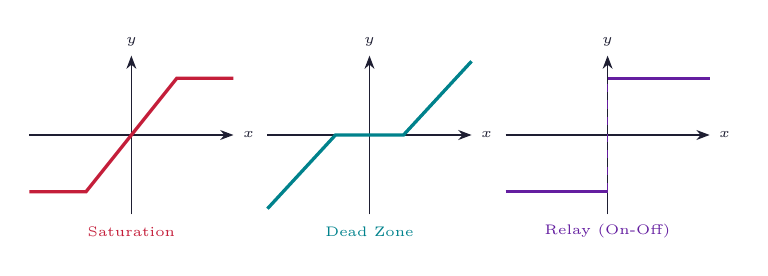
\begin{tikzpicture}[scale=0.72]
  % Saturation
  \begin{scope}[xshift=0cm]
    \draw[axis] (-1.8,0)--(1.8,0) node[right,font=\tiny]{$x$};
    \draw[axis] (0,-1.4)--(0,1.4) node[above,font=\tiny]{$y$};
    \draw[color=myred,line width=1.2pt] (-1.8,-1)--(-0.8,-1)--( 0.8,1)--(1.8,1);
    \node[font=\tiny,color=myred] at (0,-1.7) {Saturation};
  \end{scope}
  % Dead Zone
  \begin{scope}[xshift=4.2cm]
    \draw[axis] (-1.8,0)--(1.8,0) node[right,font=\tiny]{$x$};
    \draw[axis] (0,-1.4)--(0,1.4) node[above,font=\tiny]{$y$};
    \draw[color=myteal,line width=1.2pt] (-1.8,-1.3)--(-0.6,0)--(0.6,0)--(1.8,1.3);
    \node[font=\tiny,color=myteal] at (0,-1.7) {Dead Zone};
  \end{scope}
  % Relay
  \begin{scope}[xshift=8.4cm]
    \draw[axis] (-1.8,0)--(1.8,0) node[right,font=\tiny]{$x$};
    \draw[axis] (0,-1.4)--(0,1.4) node[above,font=\tiny]{$y$};
    \draw[color=mypurple,line width=1.2pt] (-1.8,-1)--(0,-1);
    \draw[color=mypurple,line width=1.2pt] (0,1)--(1.8,1);
    \draw[dashed,color=mypurple,thin] (0,-1)--(0,1);
    \node[font=\tiny,color=mypurple] at (0,-1.7) {Relay (On-Off)};
  \end{scope}
\end{tikzpicture}
\end{tcolorbox}

\subsection{Analysis Methods for Nonlinear Systems}

\begin{itemize}[leftmargin=*, itemsep=3pt]
  \item \textbf{Phase plane analysis:} Graphical method for 2nd order systems; plots $\dot{x}$ vs $x$.
  \item \textbf{Describing function method:} Frequency-domain approximation for nonlinear elements.
  \item \textbf{Lyapunov's method:} Energy-based stability analysis without solving the equations.
  \item \textbf{Linearisation:} Valid only near an operating point; uses Taylor series expansion.
\end{itemize}

%═══════════════════════════════════════════════════════════════════════════════
\section{Describing Function Method}
%═══════════════════════════════════════════════════════════════════════════════

\begin{tcolorbox}[defbox]
\textbf{Describing Function (DF):} An approximate frequency-domain representation of a nonlinear element. It is defined as the ratio of the \textit{fundamental harmonic component} of the output to the sinusoidal input, assuming the input is a pure sinusoid $x(t) = A\sin(\omega t)$.
$$N(A) = \frac{B_1 + jA_1}{A}$$
where $A_1$ and $B_1$ are the cosine and sine coefficients of the fundamental harmonic of the output.
\end{tcolorbox}

\subsection{Assumptions of the Describing Function Method}

\begin{enumerate}[label=\textbf{\arabic*.}, leftmargin=*, itemsep=3pt]
  \item The nonlinear element is \textbf{single-valued} (no memory/hysteresis) or has known hysteresis.
  \item The input to the nonlinear element is a \textbf{pure sinusoid}: $x(t) = A\sin(\omega t)$.
  \item The linear part of the system has \textbf{sufficient low-pass filtering} so that higher harmonics of the output are attenuated --- only the fundamental harmonic reaches the nonlinear element.
  \item The nonlinear element is \textbf{odd-symmetric}: $f(-x) = -f(x)$ (no even harmonics).
\end{enumerate}

\subsection{Describing Functions of Common Nonlinearities}

\begin{tabularx}{\linewidth}{|B{2.8cm}|>{\centering\arraybackslash}X|>{\raggedright\arraybackslash}X|}
\hline
\multicolumn{1}{|>{\centering\arraybackslash}p{2.8cm}|}{\textbf{\color{myteal}Nonlinearity}} &
\textbf{\color{myteal}Describing Function $N(A)$} &
\textbf{\color{myteal}Notes} \\
\hline
Ideal Relay & $\dfrac{4M}{\pi A}$ & $M$ = relay output level; real, decreases with $A$ \\
\hline
Saturation & $\displaystyle\frac{2K}{\pi}\!\left[\sin^{-1}\!\!\left(\frac{D}{A}\right)+\frac{D}{A}\sqrt{1-\left(\frac{D}{A}\right)^{\!2}}\,\right]$ & $K$ = slope, $D$ = saturation level; valid for $A>D$ \\
\hline
Dead Zone & \multicolumn{2}{>{\raggedright\arraybackslash}p{\dimexpr\linewidth-2.8cm-4\tabcolsep-3\arrayrulewidth}|}{%
  $\displaystyle K\!\left[1 - \frac{2}{\pi}\sin^{-1}\!\!\left(\frac{\Delta}{A}\right) - \frac{2\Delta}{\pi A}\sqrt{1-\left(\frac{\Delta}{A}\right)^{\!2}}\,\right]$
  \quad {\small($\Delta$ = dead zone half-width; valid for $A>\Delta$)}} \\
\hline
Backlash & Complex (has imaginary part) & Phase lag introduced; $N(A)$ is complex \\
\hline
\end{tabularx}

\subsection{Limit Cycle Prediction Using Describing Function}

The describing function method is primarily used to predict \textbf{limit cycles} --- sustained oscillations in nonlinear systems.

\begin{tcolorbox}[formulabox, title={Limit Cycle Condition}]
For a nonlinear system with nonlinear element $N(A)$ in the forward path and linear element $G(j\omega)$ in the loop, a limit cycle exists when:
$$G(j\omega)\cdot N(A) = -1 \quad \Rightarrow \quad G(j\omega) = -\frac{1}{N(A)}$$
\textbf{Graphical method:} Plot $G(j\omega)$ (Nyquist plot) and $-1/N(A)$ (negative inverse DF locus) on the same complex plane. Their \textbf{intersection} gives the limit cycle amplitude $A^*$ and frequency $\omega^*$.
\end{tcolorbox}

\begin{tcolorbox}[tikzbox, title={Limit Cycle Prediction --- Graphical Method}]
\centering
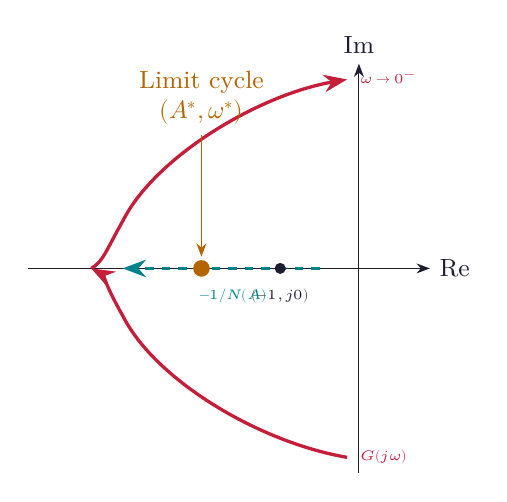
\begin{tikzpicture}[scale=1.0]
  % ── Axes ──────────────────────────────────────────────────────────────────
  \draw[-Stealth, thin, color=mydark] (-4.2,0)--(0.9,0) node[right,font=\small]{Re};
  \draw[-Stealth, thin, color=mydark] (0,-2.6)--(0,2.6) node[above,font=\small]{Im};

  % ── Nyquist plot of G(jω) — smooth Type-1 second order shape ─────────────
  % Lower half (omega: 0+ → infinity): starts at -j*infty (approx -2.4), sweeps left, ends near origin
  \draw[color=myred, line width=1.2pt, -Stealth]
    (-0.15,-2.4) .. controls (-1.3,-2.2) and (-2.6,-1.4) .. (-3.0,-0.6)
                 .. controls (-3.2,-0.25) and (-3.25,-0.08) .. (-3.4,0);
  % Upper half (mirror)
  \draw[color=myred, line width=1.2pt, -Stealth]
    (-3.4,0)     .. controls (-3.25,0.08) and (-3.2,0.25) .. (-3.0,0.6)
                 .. controls (-2.6,1.4) and (-1.3,2.2) .. (-0.15,2.4);

  % ── -1/N(A) locus (along negative real axis) ─────────────────────────────
  \draw[color=myteal, line width=1.2pt, dashed, -Stealth]
    (-0.5,0) -- (-3.0,0);

  % ── Critical (-1, j0) point ──────────────────────────────────────────────
  \fill[mydark] (-1,0) circle (2pt);
  \node[below=4pt, font=\tiny, color=mydark] at (-1,0) {$(-1, j0)$};

  % ── Limit cycle intersection ─────────────────────────────────────────────
  \fill[myamber] (-2.0,0) circle (3pt);
  % Annotation arrow + label well above the curve
  \draw[-Stealth, thin, color=myamber] (-2.0,1.7) -- (-2.0,0.15);
  \node[above, font=\small, color=myamber, align=center] at (-2.0,1.7)
    {Limit cycle\\$(A^*, \omega^*)$};

  % ── Curve labels (placed away from the action) ───────────────────────────
  \node[right, font=\tiny, color=myred] at (-0.1,-2.4) {$G(j\omega)$};
  \node[right, font=\tiny, color=myred] at (-0.1, 2.4) {$\omega \to 0^-$};
  \node[font=\tiny, color=myteal] at (-1.6,-0.35) {$-1/N(A)$};
\end{tikzpicture}
\end{tcolorbox}

\begin{tcolorbox}[exambox, title={Exam Tips --- Describing Function}]
\begin{itemize}[leftmargin=*, itemsep=3pt, topsep=0pt]
  \item DF is an \textbf{approximation} --- valid only when higher harmonics are filtered by the linear part.
  \item DF of ideal relay: $N(A) = 4M/(\pi A)$ --- purely real, decreases as $A$ increases.
  \item \textbf{Limit cycle} exists at intersection of $G(j\omega)$ and $-1/N(A)$ loci.
  \item If $-1/N(A)$ locus does \textbf{not intersect} $G(j\omega)$: no limit cycle predicted.
  \item \textbf{Stability of limit cycle:} If increasing $A$ moves $-1/N(A)$ outside $G(j\omega)$, the limit cycle is stable.
  \item DF method cannot detect \textbf{subharmonic oscillations} or \textbf{chaotic behaviour}.
\end{itemize}
\end{tcolorbox}

%═══════════════════════════════════════════════════════════════════════════════
\section{Introduction to Optimal Control}
%═══════════════════════════════════════════════════════════════════════════════

\begin{tcolorbox}[defbox]
\textbf{Optimal Control:} A control strategy that minimises (or maximises) a specified \textbf{performance index} (cost function) $J$ while satisfying the system dynamics and constraints. It provides the \textit{best possible} control in a mathematically defined sense.\\[4pt]
\textbf{Performance Index (Cost Function):} A scalar measure of system performance. Common form:
$$J = \int_0^{t_f} L(\mathbf{x}(t),\, \mathbf{u}(t),\, t)\, dt + \phi(\mathbf{x}(t_f))$$
where $L$ is the running cost and $\phi$ is the terminal cost.
\end{tcolorbox}

\subsection{Quadratic Performance Index (LQR)}

The most widely used performance index for linear systems is the \textbf{quadratic} form:

\begin{tcolorbox}[formulabox, title={Quadratic Performance Index}]
$$J = \int_0^{\infty} \left[\mathbf{x}^T(t)\,\mathbf{Q}\,\mathbf{x}(t) + \mathbf{u}^T(t)\,\mathbf{R}\,\mathbf{u}(t)\right] dt$$
where:
\begin{itemize}[leftmargin=*, itemsep=2pt, topsep=2pt]
  \item $\mathbf{Q}$ ($n\times n$, positive semi-definite) --- penalises state deviation from zero
  \item $\mathbf{R}$ ($r\times r$, positive definite) --- penalises control effort
  \item Large $\mathbf{Q}$: fast state regulation (aggressive control)
  \item Large $\mathbf{R}$: small control effort (gentle control)
\end{itemize}
The optimal control law is: $\mathbf{u}^*(t) = -\mathbf{R}^{-1}\mathbf{B}^T\mathbf{P}\,\mathbf{x}(t) = -\mathbf{K}\,\mathbf{x}(t)$\\
where $\mathbf{P}$ satisfies the \textbf{Algebraic Riccati Equation (ARE):}
$$\mathbf{A}^T\mathbf{P} + \mathbf{P}\mathbf{A} - \mathbf{P}\mathbf{B}\mathbf{R}^{-1}\mathbf{B}^T\mathbf{P} + \mathbf{Q} = \mathbf{0}$$
\end{tcolorbox}

\subsection{Regulator Problem}

\begin{tcolorbox}[defbox]
\textbf{Regulator Problem:} Drive the state $\mathbf{x}(t)$ to \textbf{zero} (or maintain it at zero) in the presence of disturbances, starting from a non-zero initial condition $\mathbf{x}(0) \neq \mathbf{0}$.\\[4pt]
\textbf{Goal:} $\mathbf{x}(t) \to \mathbf{0}$ as $t \to \infty$, while minimising the cost $J$.\\[4pt]
\textbf{Reference:} $\mathbf{r}(t) = \mathbf{0}$ (zero reference). The system must reject disturbances and return to equilibrium.\\[4pt]
\textbf{Example:} Stabilising an inverted pendulum at the upright position.
\end{tcolorbox}

\begin{tcolorbox}[tikzbox, title={Regulator Problem Block Diagram}]
\centering
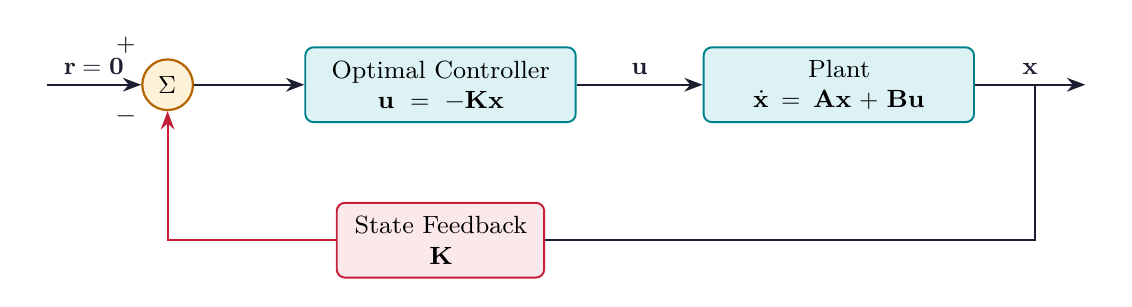
\begin{tikzpicture}[node distance=0.5cm and 1.5cm]
  \node[sumjunc] (sum) {$\Sigma$};
  \node[wblock, right=1.4cm of sum] (ctrl) {Optimal Controller\\$\mathbf{u}=-\mathbf{K}\mathbf{x}$};
  \node[wblock, right=1.6cm of ctrl] (plant) {Plant\\$\dot{\mathbf{x}}=\mathbf{A}\mathbf{x}+\mathbf{B}\mathbf{u}$};
  \node[left=1.2cm of sum] (ref) {};
  \node[right=1.4cm of plant] (out) {};
  \node[redblock, below=1.0cm of ctrl] (fb) {State Feedback\\$\mathbf{K}$};
  \draw[arrow] (ref) -- node[above]{\small $\mathbf{r}=\mathbf{0}$} (sum);
  \draw[arrow] (sum) -- (ctrl);
  \draw[arrow] (ctrl) -- node[above]{\small $\mathbf{u}$} (plant);
  \draw[arrow] (plant) -- node[above]{\small $\mathbf{x}$} (out);
  \coordinate (xtap) at ($(plant.east)!0.5!(out)$);
  \draw[line] (xtap) |- (fb.east);
  \draw[redarrow] (fb.west) -| (sum.south);
  \node[above left=1pt and 1pt of sum]{\small $+$};
  \node[below left=1pt and 1pt of sum]{\small $-$};
\end{tikzpicture}
\end{tcolorbox}

\subsection{Output Regulator Problem}

\begin{tcolorbox}[defbox]
\textbf{Output Regulator Problem:} A variant of the regulator problem where the \textbf{output} $\mathbf{y}(t)$ (not the full state) is driven to zero. The performance index penalises the output rather than the full state:
$$J = \int_0^{\infty} \left[\mathbf{y}^T\mathbf{Q}_y\mathbf{y} + \mathbf{u}^T\mathbf{R}\mathbf{u}\right] dt = \int_0^{\infty} \left[\mathbf{x}^T\mathbf{C}^T\mathbf{Q}_y\mathbf{C}\,\mathbf{x} + \mathbf{u}^T\mathbf{R}\mathbf{u}\right] dt$$
This is equivalent to the state regulator with $\mathbf{Q} = \mathbf{C}^T\mathbf{Q}_y\mathbf{C}$.\\[4pt]
\textbf{Use case:} When only the output (not all states) needs to be regulated, and full state measurement is unavailable.
\end{tcolorbox}

\subsection{Tracking Problem}

\begin{tcolorbox}[defbox]
\textbf{Tracking Problem:} The output $\mathbf{y}(t)$ must \textbf{follow} (track) a desired reference trajectory $\mathbf{r}(t) \neq \mathbf{0}$. The error $\mathbf{e}(t) = \mathbf{r}(t) - \mathbf{y}(t)$ must be minimised.\\[4pt]
\textbf{Performance index:}
$$J = \int_0^{t_f} \left[\mathbf{e}^T(t)\,\mathbf{Q}\,\mathbf{e}(t) + \mathbf{u}^T(t)\,\mathbf{R}\,\mathbf{u}(t)\right] dt$$
\textbf{Example:} Robot arm tracking a desired trajectory; missile tracking a moving target; CNC machine following a path.
\end{tcolorbox}

\begin{tabularx}{\linewidth}{|B{2.8cm}|>{\centering\arraybackslash}X|>{\centering\arraybackslash}X|>{\centering\arraybackslash}X|}
\hline
\multicolumn{1}{|>{\centering\arraybackslash}p{2.8cm}|}{\textbf{Problem}} &
\textbf{\color{myamber}Reference} & \textbf{\color{mygreen}Goal} & \textbf{\color{myteal}Example} \\
\hline
Regulator & $\mathbf{r}=\mathbf{0}$ & $\mathbf{x}(t)\to\mathbf{0}$ & Stabilise inverted pendulum \\
\hline
Output Regulator & $\mathbf{r}=\mathbf{0}$ & $\mathbf{y}(t)\to\mathbf{0}$ & Regulate output only \\
\hline
Tracking & $\mathbf{r}(t)\neq\mathbf{0}$ & $\mathbf{y}(t)\to\mathbf{r}(t)$ & Robot arm trajectory \\
\hline
\end{tabularx}

\begin{tcolorbox}[exambox, title={Exam Tips --- Optimal Control}]
\begin{itemize}[leftmargin=*, itemsep=3pt, topsep=0pt]
  \item \textbf{LQR} = Linear Quadratic Regulator; optimal for linear systems with quadratic cost.
  \item \textbf{$\mathbf{Q}$ large} $\Rightarrow$ fast state regulation; \textbf{$\mathbf{R}$ large} $\Rightarrow$ small control effort.
  \item Optimal gain: $\mathbf{K} = \mathbf{R}^{-1}\mathbf{B}^T\mathbf{P}$ where $\mathbf{P}$ solves the Algebraic Riccati Equation.
  \item \textbf{Regulator:} zero reference, drive state to zero. \textbf{Tracking:} non-zero reference, follow trajectory.
  \item \textbf{Output regulator:} only output penalised; equivalent to state regulator with $\mathbf{Q}=\mathbf{C}^T\mathbf{Q}_y\mathbf{C}$.
  \item Optimal control requires the system to be \textbf{controllable} (otherwise $J$ cannot be minimised).
\end{itemize}
\end{tcolorbox}

%═══════════════════════════════════════════════════════════════════════════════
\newpage
\begin{center}
  {\large\bfseries\color{myred} Quick Revision --- Module 6}\\[3pt]
  {\small\color{mydark} Nonlinear Systems \& Optimal Control $|$ EC601}
\end{center}
\noindent{\color{myred}\rule{\linewidth}{1.2pt}}\vspace{4pt}

\begin{tcolorbox}[formulabox, title={\textbf{Key Formulas at a Glance}}]
\begin{tabularx}{\linewidth}{B{5.0cm} X}
DF of ideal relay           & $N(A) = 4M/(\pi A)$ \\[2pt]
Limit cycle condition       & $G(j\omega) = -1/N(A)$ \\[2pt]
Quadratic cost function     & $J = \int_0^\infty (\mathbf{x}^T\mathbf{Q}\mathbf{x} + \mathbf{u}^T\mathbf{R}\mathbf{u})\,dt$ \\[2pt]
Optimal control law (LQR)   & $\mathbf{u}^* = -\mathbf{K}\mathbf{x} = -\mathbf{R}^{-1}\mathbf{B}^T\mathbf{P}\mathbf{x}$ \\[2pt]
Algebraic Riccati Eq.       & $\mathbf{A}^T\mathbf{P}+\mathbf{P}\mathbf{A}-\mathbf{P}\mathbf{B}\mathbf{R}^{-1}\mathbf{B}^T\mathbf{P}+\mathbf{Q}=\mathbf{0}$ \\[2pt]
Output regulator $\mathbf{Q}$ & $\mathbf{Q} = \mathbf{C}^T\mathbf{Q}_y\mathbf{C}$ \\[2pt]
Tracking error              & $\mathbf{e}(t) = \mathbf{r}(t) - \mathbf{y}(t)$
\end{tabularx}
\end{tcolorbox}

\vspace{5pt}

\begin{tcolorbox}[defbox, title={\textbf{One-Line Definitions}}]
\begin{itemize}[leftmargin=*, itemsep=3pt, topsep=0pt]
  \item \textbf{Nonlinear system:} Does not satisfy superposition; output depends on input magnitude.
  \item \textbf{Saturation:} Output limited to a maximum value regardless of input.
  \item \textbf{Dead zone:} No output for inputs below a threshold.
  \item \textbf{Limit cycle:} Sustained periodic oscillation in a nonlinear system.
  \item \textbf{Describing Function:} Ratio of fundamental harmonic output to sinusoidal input; $N(A)$.
  \item \textbf{Optimal control:} Minimises a performance index $J$ while satisfying system dynamics.
  \item \textbf{LQR:} Linear Quadratic Regulator; optimal state feedback for linear systems.
  \item \textbf{Regulator problem:} Drive state to zero from non-zero initial condition.
  \item \textbf{Output regulator:} Drive output (not full state) to zero.
  \item \textbf{Tracking problem:} Output must follow a non-zero reference trajectory.
  \item \textbf{Riccati equation:} Matrix equation whose solution $\mathbf{P}$ gives the optimal gain $\mathbf{K}$.
\end{itemize}
\end{tcolorbox}

\vspace{5pt}

\begin{tcolorbox}[exambox, title={\textbf{Frequently Asked / Viva Questions}}]
\begin{enumerate}[topsep=0pt, label=\textbf{Q\arabic*.}, itemsep=5pt]
  \item \Q{What is a nonlinear system?}
    A system that does not satisfy superposition (additivity + homogeneity). Its behaviour depends on input magnitude and initial conditions.
  \item \Q{Name four common nonlinearities in control systems.}
    Saturation, dead zone, backlash, relay (on-off), Coulomb friction, hysteresis.
  \item \Q{What is the Describing Function?}
    An approximate frequency-domain representation of a nonlinear element. $N(A)$ = ratio of fundamental harmonic output to sinusoidal input amplitude $A$.
  \item \Q{What is the DF of an ideal relay?}
    $N(A) = 4M/(\pi A)$, where $M$ is the relay output level. It is purely real and decreases as $A$ increases.
  \item \Q{How is a limit cycle predicted using the DF method?}
    Plot $G(j\omega)$ (Nyquist) and $-1/N(A)$ on the same complex plane. Their intersection gives the limit cycle amplitude $A^*$ and frequency $\omega^*$.
  \item \Q{What are the assumptions of the DF method?}
    Sinusoidal input to nonlinear element; linear part has sufficient low-pass filtering; nonlinearity is odd-symmetric; single-valued (or known hysteresis).
  \item \Q{What is the optimal control problem?}
    Find the control $\mathbf{u}(t)$ that minimises a performance index $J$ subject to the system dynamics $\dot{\mathbf{x}}=\mathbf{A}\mathbf{x}+\mathbf{B}\mathbf{u}$.
  \item \Q{What is the LQR cost function?}
    $J = \int_0^\infty (\mathbf{x}^T\mathbf{Q}\mathbf{x} + \mathbf{u}^T\mathbf{R}\mathbf{u})\,dt$. $\mathbf{Q}$ penalises state deviation; $\mathbf{R}$ penalises control effort.
  \item \Q{What is the regulator problem?}
    Drive the state $\mathbf{x}(t)\to\mathbf{0}$ from a non-zero initial condition, with zero reference input, while minimising $J$.
  \item \Q{What is the difference between regulator and tracking?}
    Regulator: reference is zero, goal is to drive state/output to zero. Tracking: reference is non-zero, goal is to follow the reference trajectory.
  \item \Q{What is the Algebraic Riccati Equation?}
    $\mathbf{A}^T\mathbf{P}+\mathbf{P}\mathbf{A}-\mathbf{P}\mathbf{B}\mathbf{R}^{-1}\mathbf{B}^T\mathbf{P}+\mathbf{Q}=\mathbf{0}$. Its solution $\mathbf{P}$ gives the optimal gain $\mathbf{K}=\mathbf{R}^{-1}\mathbf{B}^T\mathbf{P}$.
\end{enumerate}
\end{tcolorbox}


% -- Module 7 -----------------------------------------------------------------
\modulestart{7}{Cathode Ray Oscilloscope (CRO)}

\section{Cathode Ray Oscilloscope (CRO)}
%═══════════════════════════════════════════════════════════════════════════════

\begin{tcolorbox}[defbox]
\textbf{CRO (Cathode Ray Oscilloscope):} An electronic test instrument that displays electrical signals as waveforms on a phosphor screen. It plots voltage (Y-axis) vs time (X-axis) in real time, allowing measurement of amplitude, frequency, phase, rise time, and waveform shape.
\end{tcolorbox}

\subsection{Block Diagram of CRO}

\begin{tcolorbox}[tikzbox, title={CRO Block Diagram}]
\centering
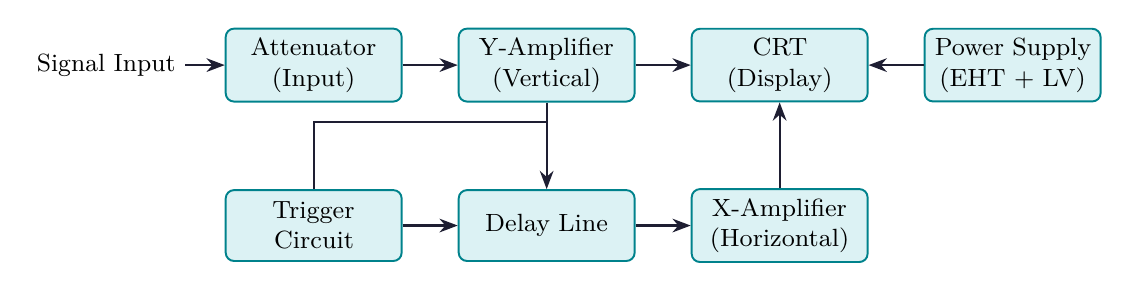
\begin{tikzpicture}[node distance=0.4cm and 0.7cm,
  sblock/.style={rectangle, draw=myteal, fill=hdrteal, text width=2.0cm,
    align=center, minimum height=0.9cm, font=\small, rounded corners=3pt, line width=0.7pt}]

  % ── Top row (left to right): Attenuator → Y-Amp → CRT ──────────────────
  \node[sblock] (atten) {Attenuator\\(Input)};
  \node[sblock, right=0.7cm of atten] (yamp)  {Y-Amplifier\\(Vertical)};
  \node[sblock, right=0.7cm of yamp]  (crt)   {CRT\\(Display)};
  \node[sblock, right=0.7cm of crt]   (psu)   {Power Supply\\(EHT + LV)};

  % ── Bottom row: Trigger → Delay → X-Amp ────────────────────────────────
  \node[sblock, below=1.1cm of atten] (trig)  {Trigger\\Circuit};
  \node[sblock, right=0.7cm of trig]  (delay) {Delay Line};
  \node[sblock, right=0.7cm of delay] (xamp)  {X-Amplifier\\(Horizontal)};

  % ── Signal path ─────────────────────────────────────────────────────────
  \draw[arrow] (atten) -- (yamp);
  \draw[arrow] (yamp)  -- (crt);
  \draw[arrow] (psu)   -- (crt);

  % ── Sweep path ──────────────────────────────────────────────────────────
  \draw[arrow] (trig)  -- (delay);
  \draw[arrow] (delay) -- (xamp);
  \draw[arrow] (xamp)  -- (crt);

  % ── Y-amp → Delay Line (vertical tap) ───────────────────────────────────
  \draw[arrow] (yamp.south) -- (delay.north);

  % ── Trigger tapped from Y-amp ────────────────────────────────────────────
  \coordinate (ytap) at ($(yamp.south)+(0,-0.25)$);
  \draw[line]  (ytap) -| (trig.north);

  % ── Input label ──────────────────────────────────────────────────────────
  \node[left=0.5cm of atten, font=\small] {Signal Input};
  \draw[arrow] ($(atten.west)-(0.5,0)$) -- (atten.west);
\end{tikzpicture}
\end{tcolorbox}

\subsection{Main Blocks and Functions}

\begin{tabularx}{\linewidth}{|B{3.2cm}|X|}
\hline
\multicolumn{1}{|>{\centering\arraybackslash}p{3.2cm}|}{\textbf{\color{myteal}Block}} &
\multicolumn{1}{>{\centering\arraybackslash}X|}{\textbf{\color{myteal}Function}} \\
\hline
Attenuator & Reduces input signal to a safe level for the amplifier. Calibrated in V/div. \\
\hline
Y-Amplifier & Amplifies the vertical (signal) input to drive the vertical deflection plates of CRT. \\
\hline
Delay Line & Delays the signal slightly so the sweep starts before the signal arrives --- ensures complete waveform display. \\
\hline
Trigger Circuit & Synchronises the sweep with the input signal to produce a stable display. \\
\hline
Time Base (Sweep Gen.) & Generates a sawtooth waveform for horizontal deflection. Calibrated in time/div. \\
\hline
X-Amplifier & Amplifies the time base signal to drive the horizontal deflection plates. \\
\hline
CRT & Cathode Ray Tube --- electron gun, deflection plates, phosphor screen. Displays the waveform. \\
\hline
Power Supply & Provides EHT ($\sim$1--10 kV) for CRT and low voltages for amplifiers. \\
\hline
\end{tabularx}

\subsection{Measurements with CRO}

\begin{tabularx}{\linewidth}{|B{3.0cm}|X|}
\hline
\multicolumn{1}{|>{\centering\arraybackslash}p{3.0cm}|}{\textbf{\color{mygreen}Measurement}} &
\multicolumn{1}{>{\centering\arraybackslash}X|}{\textbf{\color{mygreen}Method}} \\
\hline
Voltage (peak) & Count vertical divisions $\times$ V/div setting. $V_{pk} = n_{div} \times \text{V/div}$ \\
\hline
Time period $T$ & Count horizontal divisions for one cycle $\times$ time/div. $T = n_{div} \times \text{time/div}$ \\
\hline
Frequency & $f = 1/T$ \\
\hline
Phase difference & Use dual-trace mode; measure time shift $\Delta t$. $\phi = (\Delta t / T)\times 360°$ \\
\hline
Rise time & Time for signal to go from 10\% to 90\% of final value. \\
\hline
DC voltage & Set coupling to DC; measure vertical displacement from zero. \\
\hline
\end{tabularx}

%═══════════════════════════════════════════════════════════════════════════════
\section{Wave Analyzer and Spectrum Analyzer}
%═══════════════════════════════════════════════════════════════════════════════

\subsection{Wave Analyzer}

\begin{tcolorbox}[defbox]
\textbf{Wave Analyzer:} An instrument that measures the \textbf{amplitude} and \textbf{frequency} of individual harmonic components of a complex periodic waveform. It is essentially a \textit{very narrow bandpass filter} that can be tuned to any frequency within its range.
\end{tcolorbox}

\textbf{Requirements:}
\begin{itemize}[leftmargin=*, itemsep=2pt]
  \item Very narrow, stable, and tunable bandpass filter
  \item High selectivity (ability to separate closely spaced harmonics)
  \item High sensitivity (detect small amplitude components)
  \item Calibrated frequency and amplitude readout
\end{itemize}

\begin{tcolorbox}[tikzbox, title={Wave Analyzer Block Diagram}]
\centering
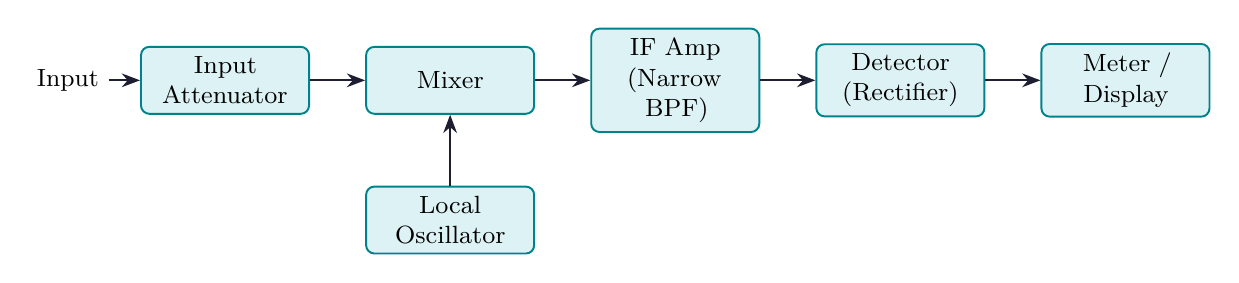
\begin{tikzpicture}[node distance=0.3cm and 0.7cm,
  sblock/.style={rectangle, draw=myteal, fill=hdrteal, text width=1.9cm,
    align=center, minimum height=0.85cm, font=\small, rounded corners=3pt, line width=0.7pt}]
  \node[sblock] (inp)   {Input\\Attenuator};
  \node[sblock, right=0.7cm of inp]   (mixer) {Mixer};
  \node[sblock, right=0.7cm of mixer] (if)    {IF Amp\\(Narrow BPF)};
  \node[sblock, right=0.7cm of if]    (det)   {Detector\\(Rectifier)};
  \node[sblock, right=0.7cm of det]   (meter) {Meter /\\Display};
  \node[sblock, below=0.9cm of mixer] (osc)   {Local\\Oscillator};

  \draw[arrow] (inp) -- (mixer);
  \draw[arrow] (mixer) -- (if);
  \draw[arrow] (if) -- (det);
  \draw[arrow] (det) -- (meter);
  \draw[arrow] (osc) -- (mixer);
  \node[left=0.4cm of inp, font=\small] {Input};
  \draw[arrow] ($(inp.west)-(0.4,0)$) -- (inp.west);
\end{tikzpicture}
\end{tcolorbox}

\subsection{Spectrum Analyzer}

\begin{tcolorbox}[defbox]
\textbf{Spectrum Analyzer:} Displays the \textbf{frequency spectrum} of a signal --- amplitude (or power) vs frequency. Unlike the wave analyzer (which measures one frequency at a time), the spectrum analyzer displays \textit{all frequency components simultaneously} on a screen (frequency domain display).
\end{tcolorbox}

\textbf{Requirements:}
\begin{itemize}[leftmargin=*, itemsep=2pt]
  \item Wide frequency range with fine resolution
  \item High dynamic range (detect weak signals near strong ones)
  \item Fast sweep speed for real-time display
  \item Calibrated frequency (X-axis) and amplitude/power (Y-axis in dBm)
\end{itemize}

\begin{tcolorbox}[tikzbox, title={Spectrum Analyzer Block Diagram (Swept Superheterodyne)}]
\centering
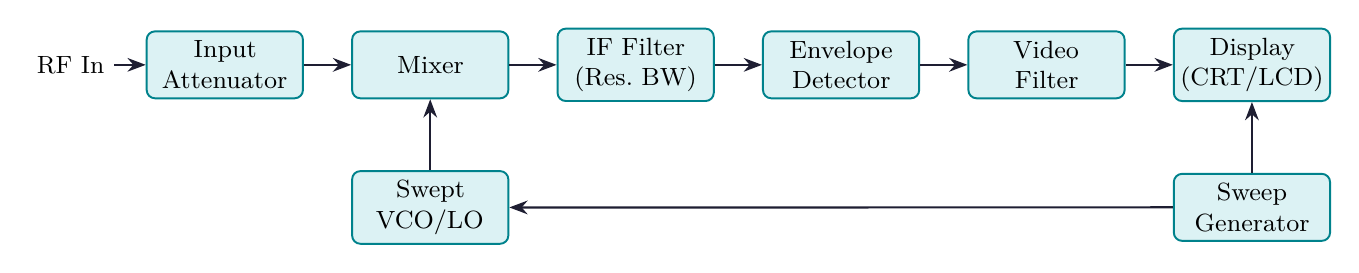
\begin{tikzpicture}[node distance=0.3cm and 0.65cm,
  sblock/.style={rectangle, draw=myteal, fill=hdrteal, text width=1.75cm,
    align=center, minimum height=0.85cm, font=\small, rounded corners=3pt, line width=0.7pt}]
  \node[sblock] (inp)  {Input\\Attenuator};
  \node[sblock, right=0.6cm of inp]  (mix)  {Mixer};
  \node[sblock, right=0.6cm of mix]  (if)   {IF Filter\\(Res.\ BW)};
  \node[sblock, right=0.6cm of if]   (det)  {Envelope\\Detector};
  \node[sblock, right=0.6cm of det]  (vbw)  {Video\\Filter};
  \node[sblock, right=0.6cm of vbw]  (disp) {Display\\(CRT/LCD)};
  \node[sblock, below=0.9cm of mix]  (vco)  {Swept\\VCO/LO};
  \node[sblock, below=0.9cm of disp] (sweep){Sweep\\Generator};

  \draw[arrow] (inp)  -- (mix);
  \draw[arrow] (mix)  -- (if);
  \draw[arrow] (if)   -- (det);
  \draw[arrow] (det)  -- (vbw);
  \draw[arrow] (vbw)  -- (disp);
  \draw[arrow] (vco)  -- (mix);
  \draw[arrow] (sweep)-- (vco);
  \draw[arrow] (sweep)-- (disp);
  \node[left=0.4cm of inp, font=\small] {RF In};
  \draw[arrow] ($(inp.west)-(0.4,0)$) -- (inp.west);
\end{tikzpicture}
\end{tcolorbox}

\begin{tabularx}{\linewidth}{|B{3.0cm}|>{\centering\arraybackslash}X|>{\centering\arraybackslash}X|}
\hline
\multicolumn{1}{|>{\centering\arraybackslash}p{3.0cm}|}{\textbf{Feature}} &
\textbf{\color{myamber}Wave Analyzer} & \textbf{\color{mygreen}Spectrum Analyzer} \\
\hline
Display & One frequency at a time & All frequencies simultaneously \\
\hline
Domain & Frequency (selective) & Frequency (full spectrum) \\
\hline
Speed & Slow (manual tuning) & Fast (swept or FFT) \\
\hline
Use & Harmonic distortion analysis & Wideband signal analysis \\
\hline
\end{tabularx}

%═══════════════════════════════════════════════════════════════════════════════
\section{LVDT (Linear Variable Differential Transformer)}
%═══════════════════════════════════════════════════════════════════════════════

\begin{tcolorbox}[defbox]
\textbf{LVDT:} A \textbf{Linear Variable Differential Transformer} is an electromechanical transducer that converts linear displacement into a proportional AC voltage. It is the most widely used inductive displacement sensor due to its high accuracy, infinite resolution, and frictionless operation.
\end{tcolorbox}

\subsection{Construction and Working}

\textbf{Construction:} One primary coil (centre) and two secondary coils (S1, S2) wound symmetrically on a cylindrical former. A movable ferromagnetic \textbf{core} (plunger) slides inside without contact.

\textbf{Working:}
\begin{enumerate}[label=\textbf{\arabic*.}, leftmargin=*, itemsep=3pt]
  \item AC excitation applied to primary coil induces EMF in both secondary coils.
  \item Secondary coils connected in \textbf{series opposition}: $V_{out} = V_{S1} - V_{S2}$.
  \item \textbf{Null position} (core centred): $V_{S1} = V_{S2}$, so $V_{out} = 0$.
  \item \textbf{Core displaced right:} $V_{S1} > V_{S2}$, $V_{out}$ is positive and in phase with primary.
  \item \textbf{Core displaced left:} $V_{S2} > V_{S1}$, $V_{out}$ is negative (180° phase shift).
\end{enumerate}

\begin{tcolorbox}[tikzbox, title={LVDT Construction and Output Characteristic}]
\centering
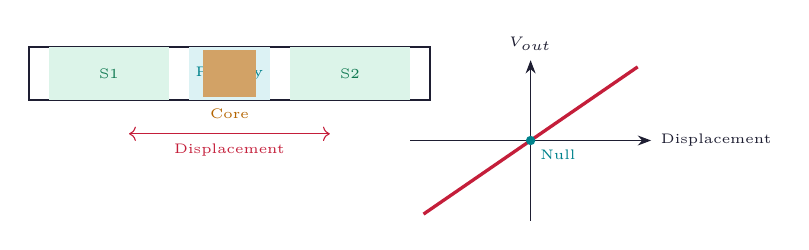
\begin{tikzpicture}[scale=0.85]
  % Former
  \draw[line width=0.7pt,color=mydark] (0,0.8) rectangle (6,1.6);
  % Primary coil (centre)
  \fill[hdrteal] (2.4,0.8) rectangle (3.6,1.6);
  \node[font=\tiny,color=myteal] at (3.0,1.2) {Primary};
  % S1
  \fill[hdrgreen] (0.3,0.8) rectangle (2.1,1.6);
  \node[font=\tiny,color=mygreen] at (1.2,1.2) {S1};
  % S2
  \fill[hdrgreen] (3.9,0.8) rectangle (5.7,1.6);
  \node[font=\tiny,color=mygreen] at (4.8,1.2) {S2};
  % Core
  \fill[myamber!60] (2.6,0.85) rectangle (3.4,1.55);
  \node[font=\tiny,color=myamber] at (3.0,0.6) {Core};
  % Displacement arrow
  \draw[<->,color=myred,thin] (1.5,0.3) -- (4.5,0.3) node[midway,below,font=\tiny] {Displacement};
  % Output characteristic
  \begin{scope}[xshift=7.5cm, yshift=0.2cm]
    \draw[-Stealth,thin,color=mydark] (-1.8,0)--(1.8,0) node[right,font=\tiny]{Displacement};
    \draw[-Stealth,thin,color=mydark] (0,-1.2)--(0,1.2) node[above,font=\tiny]{$V_{out}$};
    \draw[color=myred,line width=1.2pt] (-1.6,-1.1)--(1.6,1.1);
    \fill[myteal] (0,0) circle (2pt);
    \node[below right,font=\tiny,color=myteal] at (0,0) {Null};
  \end{scope}
\end{tikzpicture}
\end{tcolorbox}

\begin{tabularx}{\linewidth}{|>{\centering\arraybackslash}X|>{\centering\arraybackslash}X|}
\hline
\textbf{\color{mygreen}Advantages} & \textbf{\color{myred}Disadvantages} \\
\hline
Infinite resolution (frictionless) & Sensitive to stray magnetic fields \\
\hline
High accuracy and repeatability & Requires AC excitation and demodulator \\
\hline
No mechanical wear (contactless) & Limited to linear displacement \\
\hline
Rugged; works in harsh environments & Bulkier than resistive sensors \\
\hline
\end{tabularx}

%═══════════════════════════════════════════════════════════════════════════════
\section{Servomotors}
%═══════════════════════════════════════════════════════════════════════════════

\begin{tcolorbox}[defbox]
\textbf{Servomotor:} A motor specifically designed for use in \textbf{closed-loop control systems} (servo systems). It must have a linear torque-speed characteristic, low inertia, fast response, and be controllable by an error signal. Used for precise position, speed, or torque control.
\end{tcolorbox}

\subsection{DC Servomotor}

\begin{tcolorbox}[defbox]
\textbf{DC Servomotor:} A DC motor with a separately excited field or permanent magnet field, controlled by varying the \textbf{armature voltage}. The torque is proportional to armature current; speed is proportional to back-EMF.
\end{tcolorbox}

\begin{tcolorbox}[formulabox, title={DC Servomotor Equations}]
\textbf{Electrical:} $V_a = E_b + I_a R_a + L_a \dfrac{dI_a}{dt}$, \quad $E_b = K_b\,\omega$\\[4pt]
\textbf{Mechanical:} $T = K_T\,I_a = J\dfrac{d\omega}{dt} + B\,\omega$\\[4pt]
\textbf{Transfer Function} (armature control, $L_a \approx 0$):
$$\frac{\Omega(s)}{V_a(s)} = \frac{K_T/R_a}{Js + B + K_TK_b/R_a}$$
where $K_T$ = torque constant, $K_b$ = back-EMF constant, $J$ = inertia, $B$ = damping.
\end{tcolorbox}

\begin{tabularx}{\linewidth}{|B{3.0cm}|X|}
\hline
\multicolumn{1}{|>{\centering\arraybackslash}p{3.0cm}|}{\textbf{\color{myteal}Feature}} &
\multicolumn{1}{>{\centering\arraybackslash}X|}{\textbf{\color{myteal}DC Servomotor}} \\
\hline
Control method & Armature voltage control or field control \\
\hline
Torque-speed & Linear (ideal for servo use) \\
\hline
Response & Fast; low inertia rotor \\
\hline
Maintenance & Brushes require periodic replacement \\
\hline
Applications & Robotics, CNC machines, antenna positioning \\
\hline
\end{tabularx}

\subsection{AC Servomotor}

\begin{tcolorbox}[defbox]
\textbf{AC Servomotor:} A two-phase induction motor used in servo systems. One phase (reference phase) is supplied with a fixed AC voltage; the other phase (control phase) receives a variable voltage proportional to the error signal. Speed and direction are controlled by the magnitude and phase of the control voltage.
\end{tcolorbox}

\begin{tcolorbox}[formulabox, title={AC Servomotor Key Features}]
\begin{itemize}[leftmargin=*, itemsep=2pt, topsep=2pt]
  \item \textbf{High rotor resistance:} Ensures stable, linear torque-speed characteristic (negative slope throughout).
  \item \textbf{Low inertia:} Drag-cup or thin-disc rotor for fast response.
  \item \textbf{Control:} Vary amplitude of control phase voltage; direction by phase reversal ($\pm 90°$).
  \item \textbf{Transfer function:} $G(s) = K_m / (s(\tau_m s + 1))$ where $K_m$ = motor gain, $\tau_m$ = mechanical time constant.
\end{itemize}
\end{tcolorbox}

\begin{tabularx}{\linewidth}{|B{3.0cm}|>{\centering\arraybackslash}X|>{\centering\arraybackslash}X|}
\hline
\multicolumn{1}{|>{\centering\arraybackslash}p{3.0cm}|}{\textbf{Feature}} &
\textbf{\color{myamber}DC Servomotor} & \textbf{\color{mygreen}AC Servomotor} \\
\hline
Supply & DC & 2-phase AC \\
\hline
Control & Armature voltage & Control phase voltage \\
\hline
Maintenance & Brushes needed & Brushless (robust) \\
\hline
Power range & High power & Low to medium power \\
\hline
Noise & More (brushes) & Less \\
\hline
Applications & Heavy-duty servo & Instruments, light servo \\
\hline
\end{tabularx}

%═══════════════════════════════════════════════════════════════════════════════
\section{Tachogenerator (Tacho Generator)}
%═══════════════════════════════════════════════════════════════════════════════

\begin{tcolorbox}[defbox]
\textbf{Tachogenerator:} A transducer that converts \textbf{rotational speed} into a proportional electrical voltage. Used as a \textbf{velocity feedback sensor} in closed-loop speed control systems.\\[4pt]
\textbf{DC Tacho:} Output DC voltage proportional to speed: $V_{out} = K_t\,\omega$\\[4pt]
\textbf{AC Tacho:} Output AC voltage whose amplitude is proportional to speed; frequency equals shaft rotation frequency.
\end{tcolorbox}

\begin{tabularx}{\linewidth}{|B{3.0cm}|>{\centering\arraybackslash}X|>{\centering\arraybackslash}X|}
\hline
\multicolumn{1}{|>{\centering\arraybackslash}p{3.0cm}|}{\textbf{Feature}} &
\textbf{\color{myamber}DC Tachogenerator} & \textbf{\color{mygreen}AC Tachogenerator} \\
\hline
Output & DC voltage $\propto$ speed & AC voltage amplitude $\propto$ speed \\
\hline
Direction sensing & Polarity reversal & Phase reversal \\
\hline
Ripple & Present (commutator) & None \\
\hline
Use & Speed feedback in DC drives & AC servo systems \\
\hline
\end{tabularx}

%═══════════════════════════════════════════════════════════════════════════════
\section{Hydraulic and Pneumatic Actuators}
%═══════════════════════════════════════════════════════════════════════════════

\subsection{Electro-Hydraulic Valve}

\begin{tcolorbox}[defbox]
\textbf{Electro-Hydraulic Valve (EHV):} Converts an \textbf{electrical signal} (current or voltage) into a \textbf{hydraulic flow} or pressure. It controls the flow of hydraulic fluid to an actuator. Types: servo valve (proportional), solenoid valve (on-off).\\[4pt]
\textbf{Working:} An electrical torque motor deflects a flapper between two nozzles, creating a differential pressure that positions a spool valve, which controls hydraulic flow to the actuator.
\end{tcolorbox}

\begin{tcolorbox}[tikzbox, title={Electro-Hydraulic Servo Valve (Flapper-Nozzle Type)}]
\centering
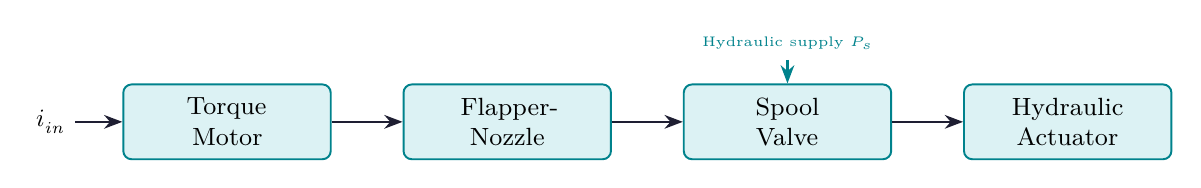
\begin{tikzpicture}[node distance=0.4cm and 1.0cm]
  \node[block] (torque) {Torque\\Motor};
  \node[block, right=0.9cm of torque] (flapper) {Flapper-\\Nozzle};
  \node[block, right=0.9cm of flapper] (spool) {Spool\\Valve};
  \node[block, right=0.9cm of spool] (act) {Hydraulic\\Actuator};
  \node[left=0.6cm of torque, font=\small] {$i_{in}$};
  \draw[arrow] ($(torque.west)-(0.6,0)$) -- (torque.west);
  \draw[arrow] (torque) -- (flapper);
  \draw[arrow] (flapper) -- (spool);
  \draw[arrow] (spool) -- (act);
  \node[above=0.3cm of spool, font=\tiny, color=myteal] {Hydraulic supply $P_s$};
  \draw[arrow,color=myteal] ($(spool.north)+(0,0.3)$) -- (spool.north);
\end{tikzpicture}
\end{tcolorbox}

\subsection{Hydraulic Servomotor}

\begin{tcolorbox}[defbox]
\textbf{Hydraulic Servomotor:} A hydraulic actuator (linear cylinder or rotary motor) that converts \textbf{hydraulic power} (pressure $\times$ flow) into \textbf{mechanical motion}. Controlled by an electro-hydraulic valve.\\[4pt]
\textbf{Advantages:} Very high force/torque output; fast response; high power-to-weight ratio.\\
\textbf{Disadvantages:} Requires hydraulic power supply; risk of leakage; maintenance intensive.
\end{tcolorbox}

\begin{tcolorbox}[formulabox, title={Hydraulic Actuator Transfer Function}]
For a hydraulic cylinder with spool valve:
$$\frac{X(s)}{I(s)} = \frac{K_h}{s(Ms + B)}$$
where $K_h$ = hydraulic gain, $M$ = load mass, $B$ = viscous damping, $X$ = piston displacement, $I$ = input current to valve.
\end{tcolorbox}

\subsection{Electro-Pneumatic Valve}

\begin{tcolorbox}[defbox]
\textbf{Electro-Pneumatic Valve:} Converts an \textbf{electrical signal} into a \textbf{pneumatic pressure or flow}. Used to control pneumatic actuators. Types: I/P converter (current-to-pressure), solenoid valve.\\[4pt]
\textbf{I/P Converter:} Converts 4--20 mA current signal to 3--15 psi (or 0.2--1.0 bar) pneumatic output. Standard interface between electronic controllers and pneumatic actuators in process industries.
\end{tcolorbox}

\subsection{Pneumatic Actuator}

\begin{tcolorbox}[defbox]
\textbf{Pneumatic Actuator:} Converts \textbf{compressed air pressure} into \textbf{mechanical motion} (linear or rotary). Controlled by an electro-pneumatic valve or I/P converter.\\[4pt]
\textbf{Types:}
\begin{itemize}[leftmargin=*, itemsep=2pt, topsep=2pt]
  \item \textbf{Spring-return diaphragm actuator:} Air pressure acts on a diaphragm against a spring. Used for control valves. Fail-safe (spring returns to safe position on air failure).
  \item \textbf{Double-acting cylinder:} Air applied alternately to both sides of a piston for bidirectional motion.
  \item \textbf{Rotary vane actuator:} Converts air pressure to rotary motion (limited angle).
\end{itemize}
\end{tcolorbox}

\begin{tabularx}{\linewidth}{|B{3.0cm}|>{\centering\arraybackslash}X|>{\centering\arraybackslash}X|>{\centering\arraybackslash}X|}
\hline
\multicolumn{1}{|>{\centering\arraybackslash}p{3.0cm}|}{\textbf{Feature}} &
\textbf{\color{myamber}Hydraulic} & \textbf{\color{mygreen}Pneumatic} & \textbf{\color{myteal}Electric} \\
\hline
Power density & Very high & Medium & Medium \\
\hline
Speed & Fast & Very fast & Fast \\
\hline
Precision & High & Moderate & Very high \\
\hline
Maintenance & High (leaks) & Low & Low \\
\hline
Compressibility & Incompressible & Compressible & N/A \\
\hline
Typical use & Heavy machinery & Process valves & Robotics, CNC \\
\hline
\end{tabularx}

%═══════════════════════════════════════════════════════════════════════════════
\newpage
\begin{center}
  {\large\bfseries\color{myred} Quick Revision --- Module 7}\\[3pt]
  {\small\color{mydark} Instrumentation \& Actuators $|$ EC601}
\end{center}
\noindent{\color{myred}\rule{\linewidth}{1.2pt}}\vspace{4pt}

\begin{tcolorbox}[formulabox, title={\textbf{Key Formulas at a Glance}}]
\begin{tabularx}{\linewidth}{B{5.0cm} X}
CRO voltage measurement     & $V_{pk} = n_{div} \times \text{V/div}$ \\[2pt]
CRO time period             & $T = n_{div} \times \text{time/div}$ \\[2pt]
CRO frequency               & $f = 1/T$ \\[2pt]
CRO phase difference        & $\phi = (\Delta t / T)\times 360°$ \\[2pt]
LVDT output                 & $V_{out} = V_{S1} - V_{S2}$; zero at null position \\[2pt]
DC tacho output             & $V_{out} = K_t\,\omega$ \\[2pt]
DC servomotor TF            & $\Omega(s)/V_a(s) = (K_T/R_a)/(Js+B+K_TK_b/R_a)$ \\[2pt]
AC servomotor TF            & $G(s) = K_m/[s(\tau_m s+1)]$ \\[2pt]
Hydraulic actuator TF       & $X(s)/I(s) = K_h/[s(Ms+B)]$ \\[2pt]
I/P converter range         & 4--20 mA $\to$ 3--15 psi (0.2--1.0 bar)
\end{tabularx}
\end{tcolorbox}

\vspace{5pt}

\begin{tcolorbox}[defbox, title={\textbf{One-Line Definitions}}]
\begin{itemize}[leftmargin=*, itemsep=3pt, topsep=0pt]
  \item \textbf{CRO:} Displays voltage vs time waveforms; measures amplitude, frequency, phase, rise time.
  \item \textbf{Trigger circuit:} Synchronises CRO sweep with input signal for stable display.
  \item \textbf{Delay line:} Delays signal in CRO so sweep starts before signal arrives.
  \item \textbf{Wave analyzer:} Measures amplitude of individual harmonics; narrow tunable BPF.
  \item \textbf{Spectrum analyzer:} Displays full frequency spectrum (amplitude vs frequency) simultaneously.
  \item \textbf{LVDT:} Inductive displacement sensor; output voltage proportional to core displacement.
  \item \textbf{Null position (LVDT):} Core centred; $V_{S1}=V_{S2}$; $V_{out}=0$.
  \item \textbf{DC servomotor:} DC motor for servo use; controlled by armature voltage; linear torque-speed.
  \item \textbf{AC servomotor:} 2-phase induction motor; high rotor resistance; low inertia; drag-cup rotor.
  \item \textbf{Tachogenerator:} Speed-to-voltage transducer; used as velocity feedback sensor.
  \item \textbf{Electro-hydraulic valve:} Converts electrical signal to hydraulic flow; flapper-nozzle type.
  \item \textbf{Hydraulic servomotor:} High-force actuator; converts hydraulic power to mechanical motion.
  \item \textbf{I/P converter:} Converts 4--20 mA to 3--15 psi; interfaces electronic controller to pneumatic actuator.
  \item \textbf{Pneumatic actuator:} Converts compressed air to mechanical motion; spring-return is fail-safe.
\end{itemize}
\end{tcolorbox}

\vspace{5pt}

\begin{tcolorbox}[exambox, title={\textbf{Frequently Asked / Viva Questions}}]
\begin{enumerate}[topsep=0pt, label=\textbf{Q\arabic*.}, itemsep=5pt]
  \item \Q{What is the function of the trigger circuit in a CRO?}
    It synchronises the time base sweep with the input signal so that the waveform appears stationary (stable) on the screen.
  \item \Q{Why is a delay line used in a CRO?}
    To delay the signal slightly so the sweep generator starts before the signal arrives, ensuring the leading edge of the waveform is displayed.
  \item \Q{How do you measure frequency using a CRO?}
    Measure the time period $T$ (horizontal divisions $\times$ time/div for one complete cycle), then $f = 1/T$.
  \item \Q{What is the difference between a wave analyzer and a spectrum analyzer?}
    Wave analyzer measures one frequency component at a time (narrow tunable BPF). Spectrum analyzer displays all frequency components simultaneously on screen.
  \item \Q{What is LVDT and how does it work?}
    Linear Variable Differential Transformer. AC excitation on primary induces EMF in two secondary coils connected in series opposition. Output voltage is proportional to core displacement; zero at null position.
  \item \Q{What is the output of LVDT at null position?}
    Zero, because the two secondary voltages are equal and opposite ($V_{S1} = V_{S2}$, so $V_{out} = V_{S1} - V_{S2} = 0$).
  \item \Q{What are the advantages of LVDT?}
    Infinite resolution (frictionless/contactless), high accuracy, no mechanical wear, rugged, works in harsh environments.
  \item \Q{What is the difference between DC and AC servomotor?}
    DC: controlled by armature voltage, uses brushes, high power. AC: 2-phase induction, brushless, high rotor resistance for linear torque-speed, low inertia drag-cup rotor.
  \item \Q{What is a tachogenerator?}
    A speed transducer that generates a voltage proportional to rotational speed ($V = K_t\omega$). Used as velocity feedback in closed-loop speed control.

  \item \Q{What is an electro-hydraulic servo valve?}
    Converts electrical current to hydraulic flow using a torque motor, flapper-nozzle, and spool valve. Controls hydraulic actuator position/speed.
  \item \Q{What is an I/P converter?}
    Current-to-pressure converter. Converts 4--20 mA electrical signal to 3--15 psi pneumatic signal. Standard interface between electronic controllers and pneumatic actuators.
  \item \Q{Why is a spring-return pneumatic actuator called fail-safe?}
    On loss of air supply, the spring returns the actuator (and connected valve) to a predetermined safe position (fully open or fully closed).
\end{enumerate}
\end{tcolorbox}


\end{document}
